% !TEX root = main.tex
\chapter{Logic and Proof}\label{C-logic}\label{C-proof}

\index{logical deduction|see{deduction}}
\index{formal proof|see{proof}}
\index{DNF|see{disjunctive normal form}}
\index{CNF|see{conjunctive normal form}}

\startchapter{In a sense, we know }a lot more than we realize,
because everything that we know has consequences---\emph{logical} 
consequences---that follow automatically.  If you know that all
humans are mortal, and you know that you are human, then in a
sense you know that you are mortal, whether or not you have ever
considered or wanted to consider that fact.  This is an example
of \nw[deduction]{logical deduction}: From the \nw[premise]{premises} that ``All
humans are mortal'' and ``I am human,'' the \nw{conclusion}
that ``I am mortal'' can be deduced by logic.

Logical deduction is a kind of computation.  By applying rules
of logic to a given set of premises, conclusions that follow
from those premises can be generated automatically, by a
computational process which could be carried out by a computer.
Once you know the premises, or are willing to accept them for
the sake of argument, you are forced---by logic---to accept
the conclusions.  Still, to say that you ``know'' those conclusions
would be misleading.  The problem is that there are too many of
them (infinitely many), and, in general, most of them are not
particularly interesting.  Until you have actually made the 
deduction, you don't \emph{really} know the conclusion, and 
knowing which of the possible chains of deduction to follow
is not easy.  The \emph{art} of logic is to find
an interesting conclusion and a chain of logical deductions that
leads from the premises to that conclusion.  Checking that the
deductions are valid is the mechanical, computational side of
logic.

This chapter is mostly about the mechanics of logic.  We will 
investigate logic as a branch of mathematics, with its own
symbols, formulas, and rules of computation.  Your object is
to learn the rules of logic, to understand why they are valid,
and to develop skill in applying them.  As with any branch of
mathematics, there is a certain beauty to the symbols and formulas
themselves.  But it is the applications that bring the subject to
life for most people.  We will, of course, cover some applications
as we go along.   In a sense, though, the real applications of
logic include much of computer science and of mathematics itself.\looseness=-1

Among the fundamental elements of thought, and therefore of logic, are
propositions.  A \nw{proposition} is a statement that has a truth
value:  It is either true or false.
``Grass is green'' and ``$2 + 2 = 5$''
are propositions.  In the first part of this chapter, we will
study \nw{propositional logic}, which takes propositions as basic
and considers how they can be combined and manipulated.  This 
branch of logic has surprising application to the design of
the electronic circuits that make up computers.

Logic gets more interesting when we consider the internal
structure of propositions.  In English, a proposition is expressed as
a sentence, and, as you know from studying grammar, sentences have
parts.  A simple sentence like ``Grass is green'' has a
\nw[none]{subject} and a \nw{predicate}.  The sentence says something
about its subject.  The subject of ``Grass is green'' is grass.
The sentence says something about grass.  The \emph{something}
that the sentence says about its subject is the predicate.
In the example, the predicate is the phrase ``is green.''
Once we start working with predicates, we can create propositions
using \nw[quantifier]{quantifiers} like ``all,'' ``some,'' and ``no.''
For example, working with the predicate ``is above average,''
we can move from simple propositions like ``Johnny is above
average'' to ``All children are above average'' or to
``No child is above average'' or to the rather more realistic
``Some children are above average.''  Logical deduction usually
deals with quantified statements, as shown by the basic example of
human mortality with which we began this chapter.  Logical deduction
will be a major topic of this chapter;  under the name of
\nw{proof}, it will be the last major topic of this chapter,
and a major tool for the
rest of this book.



\section{Propositional Logic}\label{S-logic-1}
A proposition\index{proposition}\index{propositional logic}
is a statement which is either true or false.
In propositional logic, we take propositions as basic and
see what we can do with them.  Since this is mathematics, we
need to be able to talk about propositions without saying
which particular propositions we are talking about, so we 
use symbolic names to represent them.  We will always use
lowercase letters such as $p$, $q$, and $r$ to represent
propositions.  A letter used in this way is called a
\nw[variable!propositional]{propositional variable}.  Remember that when I say
something like  ``Let $p$ be a proposition,'' I mean ``For the rest of
this discussion, let the symbol $p$ stand for some particular
statement, which is either true or false (although I am not
at the moment making any assumption about which it is).''
The discussion has \nw{mathematical generality} in that
$p$ can represent any statement, and the discussion will be
valid no matter which statement it represents.

What we do with propositions is combine them with
\nw[logical operator]{logical operators}.  A logical operator can be
applied to one or more propositions to produce a new proposition.
The truth value of the new proposition is completely determined
by the operator and by the truth values of the propositions
to which it is applied.\footnote{It is not always true that the
truth value of a sentence can be determined from the truth values
of its component parts.  For example, if $p$ is a proposition,
then ``Sarah Palin\index{Palin, Sarah} believes $p$'' is also a proposition,
so ``Sarah Palin believes'' is some kind of operator.
However, it does not count as a \emph{logical} operator because
just from knowing whether or not $p$ is true, we get no information
at all about whether ``Sarah Palin believes $p$'' is true.}
In English, logical operators are represented by words such
as ``and,'' ``or,'' and ``not.''  For example, the
proposition ``I wanted to leave and I left'' is formed from
two simpler propositions joined by the word ``and.''  Adding
the word ``not'' to the proposition ``I left'' gives
``I did not leave'' (after a bit of necessary grammatical adjustment).

But English is a little too rich for mathematical logic.
When you read the sentence ``I wanted to leave and I left,''
you probably see a connotation of causality:  I left \emph{because}
I wanted to leave.  This implication does not follow from the
logical combination of the truth values of the two propositions
``I wanted to leave'' and ``I left.'' Or consider the
proposition ``I wanted to leave but I did not leave.''
Here, the word ``but'' has the same \emph{logical} meaning
as the word ``and,'' but the connotation is very different.
So, in mathematical logic, we use \emph{symbols} to represent
logical operators.  These symbols do not carry any connotation
beyond their defined logical meaning.  The logical operators
corresponding to the English words ``and,'' ``or,''and ``not'' 
are $\AND$, $\OR$, and $\NOT$.

\begin{definition}
Let $p$ and $q$ be propositions.  Then $p\OR q$, $p \AND q$, and
$\NOT p$ are propositions, whose truth values are given by the
rules:\index{and (logical operator)}\index{or (logical operator)}\index{not (logical operator)}
\begin{itemize}
\item $p\AND q$ is true when both $p$ is true and $q$ is true, and in 
no other case.
\item $p\OR q$ is true when either $p$ is true, or $q$ is true, or both
$p$ and $q$ are true, and in no other case.
\item$\NOT p$ is true when $p$ is false, and in no other case.
\end{itemize}
The operators $\AND$, $\OR$, and $\NOT$ are referred to as \nw{conjunction},
\nw{disjunction}, and \nw{negation}, respectively.
(Note that $p\AND q$ is read as ``$p$ and $q$,'' $p\OR q$ is read
as ``$p$ or $q$,'' and $\NOT p$ is read as ``not $p$.'')
\end{definition}


These operators can be used in more complicated expressions,
such as $p\AND(\NOT q)$ or $(p\OR q)\AND(q\OR r)$.  A
proposition made up of simpler propositions and logical operators
is called a \nw{compound proposition}.  Parentheses can be used
in compound expressions to indicate the order in which the
operators are to be evaluated.  In the absence of parentheses,
the order of evaluation is determined by \nw[precedence rule]{precedence rules}.
For the logical operators defined above, the rules are that
$\NOT$ has higher precedence that $\AND$, and $\AND$ has precedence
over $\OR$.  This means that in the absence of parentheses,
any $\NOT$ operators are evaluated first, followed by any
$\AND$ operators, followed by any $\OR$ operators.

For example, the expression $\NOT p \OR q \AND r$ is
equivalent to the expression $(\NOT p)\OR (q\AND r)$,
while $p\OR q \AND q \OR r$ is equivalent to
$p \OR (q \AND q) \OR r$.  As a practical matter, when you make
up your own expressions, it is usually better to put in parentheses
to make your meaning clear.  Remember that even if you leave out
parentheses, your expression has an unambiguous meaning.
If you say ``$\NOT p \AND q$'' when what you meant was
``$\NOT (p\AND q)$,'' you've got it wrong!

This still leaves open the question of which of the $\AND$ operators
in the expression $p\AND q \AND r$ is evaluated first.
This is settled by the following rule:  When several operators
of equal precedence occur in the absence of parentheses, they
are evaluated from left to right.  Thus, the expression
$p\AND q\AND r$ is equivalent to $(p\AND q)\AND r$
rather than to $p\AND(q\AND r)$.
In this particular case, as a matter of fact, it doesn't really matter
which $\AND$ operator is evaluated first, since 
the two compound propositions $(p\AND q)\AND r$ and
$p\AND (q\AND r)$ always have the same value,
no matter what logical values the component propositions $p$,
$q$, and $r$ have.  We say that $\AND$ is an
\nw[associative operator]{associative} operation.  We'll see more about associativity
and other properties of operations in the next section.

Suppose we want to verify that, in fact, $(p\AND q)\AND r$ and
$p\AND (q\AND r)$ do always have the same value.  To do so,
we have to consider all possible combinations of values
of $p$, $q$, and $r$, and check that for all such combinations,
the two compound expressions do indeed have the same value.
It is convenient to organize this computation into a
truth table.  A \nw{truth table} is a table that shows the
value of one or more compound propositions for each possible
combination of values of the propositional variables that they contain.
Figure~\ref{F-assoc1} is a truth table that compares the
value of $(p\AND q)\AND r$ to the value of $p\AND (q\AND r)$
for all possible values of $p$, $q$, and $r$.  There are
eight rows in the table because there are exactly eight different
ways in which truth values can be assigned to $p$, $q$, and
$r$.\footnote{In general, if there are $n$ variables, then
there are $2^n$ different ways to assign truth values to the
variables.  This might become clear to you if you try to come
up with a scheme for systematically listing all possible sets
of values.  If not, you'll find a rigorous proof of the fact 
later in this chapter.}  In this table, we see that the last
two columns, representing the values of
$(p\AND q)\AND r$ and $p\AND (q\AND r)$, are
identical.

\fig
  {F-assoc1}
  {A truth table that demonstrates the logical equivalence of
      $(p\AND q)\AND r$ and $p\AND(q\AND r)$.  The fact that the
      last two columns of this table are identical shows that
      these two expressions have the same value for all eight
      possible combinations of values of $p$, $q$, and $r$.}
  {\begin{tabular}{|c|c|c||c|c|c|c|}
        \hline
        $p$& $q$& $r$&
           $p\AND q$& $q\AND r$&
           $(p\AND q)\AND r$& $p\AND (q\AND r)$\\
        \hline
        \strut false& false& false& false& false& false& false\\
        false& false& true&  false& false& false& false\\
        false& true&  false& false& false& false& false\\
        false& true&  true&  false& true&  false& false\\
        true&  false& false& false& false& false& false\\
        true&  false& true&  false& false& false& false\\
        true&  true&  false& true&  false& false& false\\
        true&  true&  true&  true&  true&  true&  true\\
        \hline
     \end{tabular}
   }

More generally, we say that two compound propositions are
\nw[logical equivalence]{logically equivalent} if they always have the same value,
no matter what truth values are assigned to the propositional
variables that they contain.  If the number of propositional
variables is small, it is easy to use a truth table to check
whether or not two propositions are logically equivalent.

\medbreak

There are other logical operators besides $\AND$, $\OR$, and
$\NOT$.  We will consider the \nw{conditional
operator}, $\IMP$, the \nw{biconditional operator}, $\IFF$,
and the \nw{exclusive or operator}, $\XOR$.\footnote{Note that the
symbols used in this book for the logical operators are not
universal.  While $\AND$, $\OR$, and $\IMP$ are fairly standard,
$\NOT$ is often replaced by $\sim$ and $\IFF$ is sometimes represented
by $\equiv$ or $\Leftrightarrow$.  There is even less standardization
of the exclusive or operator, but that operator is generally not
so important as the others.}  These operators
can be completely defined by a truth table that shows their
values for the four possible combinations
of truth values of $p$ and $q$.

\begin{definition}
For any propositions $p$ and $q$, we define the propositions
$p\IMP q$, $p\IFF q$, and $p\XOR q$ according to the truth table:
   \begin{center}
     \begin{tabular}{|c|c||c|c|c|}
        \hline
        $p$& $q$& $p\IMP q$& $p\IFF q$& $p\XOR q$\\
        \hline
        \strut false&  false&  true&   true&   false\\
        false&  true&   true&   false&  true\\
        true&   false&  false&  false&  true\\
        true&   true&   true&   true&   false\\
        \hline
      \end{tabular}
   \end{center}
\end{definition}

When these operators are used in expressions, in the absence of parentheses
to indicate order of evaluation, we use the following precedence rules:\index{precedence rule}
The exclusive or operator, $\XOR$, has the same precedence as~$\OR$.  The
conditional operator, $\IMP$, has lower precedence than
$\AND$, $\OR$, $\NOT$, and $\XOR$, and is therefore evaluated after
them.  Finally, the biconditional operator, $\IFF$, has the lowest
precedence and is therefore evaluated last.  For example,
the expression ``$p\IMP q \AND r \IFF \NOT p \XOR s$'' is evaluated
as if it were written ``$(p\IMP (q\AND r))\IFF((\NOT p) \XOR s)$.''

In order to work effectively with the logical operators, you need
to know more about their meaning and how they relate to ordinary 
English expressions.

\medbreak

The proposition $p\IMP q$ is called
an \nw{implication} or a \nw{conditional}.  It is usually
read as ``$p$ implies $q$.''
In English, $p\IMP q$ is often expressed as ``if $p$ then $q$.''
For example, if $p$ represents the proposition ``Bill Gates\index{Gates, Bill} is poor''
and $q$ represents ``the moon is made of green cheese,'' then $p\IMP q$
could be expressed in English as ``If Bill Gates is poor,
then the moon is made of green cheese.''  In this example, $p$ is
false and $q$ is also false.  Checking the definition of $p\IMP q$,
we see that $p\IMP q$ is a true statement.  Most people would agree
with this.  It's worth looking at a similar example in more detail.
Suppose that I assert that ``If the Mets\index{Mets} are a great team, then
I'm the king of France.''  This statement has the form $m\IMP k$
where $m$ is the proposition ``the Mets are a great team'' and $k$
is the proposition ``I'm the king of France.''  Now, demonstrably
I am not the king of France, so $k$ is false.  Since $k$ is false,
the only way for $m\IMP k$ to be true is for $m$ to be false as well.
(Check the definition of $\IMP$ in the table!)
So, by asserting $m\IMP k$, I am really asserting that the Mets are
\emph{not} a great team.

Or consider the statement, ``If the party is on Tuesday, then I'll
be there.''  What am I trying to say if I assert this statement?
I am asserting that $p\IMP q$ is true, where $p$ represents ``The party
is on Tuesday'' and $q$ represents ``I will be at the party.''
Suppose that $p$ is true, that is, the party does in fact take place
on Tuesday.  Checking the definition of $\IMP$, we see that in the
only case where $p$ is true and $p\IMP q$ is true, $q$ is also true.
So from the truth of ``If the party is on Tuesday, then I will be at the party''
and ``The party is in fact on Tuesday,'' you can deduce that
``I will be at the party'' is also true.  But suppose, on the other
hand, that the party is actually on Wednesday.  Then $p$ is false.
When $p$ is false and $p\IMP q$ is true, the definition of $p\IMP q$ 
allows $q$ to be either true or false.  So, in this case, you can't
make any deduction about whether or not I will be at the party.
The statement ``If the party is on Tuesday, then I'll be there''
doesn't assert anything about what will happen if the party is on
some other day than Tuesday.

The implication $(\NOT q)\IMP(\NOT p)$ is called the \nw{contrapositive}
of $p\IMP q$.  An implication is logically equivalent
to its contrapositive.  The contrapositive of ``If this is Tuesday,
then we are in Belgium'' is ``If we aren't in Belgium, then this
isn't Tuesday.''  These two sentences assert exactly the same
thing.

Note that $p\IMP q$ is \emph{not} logically equivalent to
$q\IMP p$.  The implication $q\IMP p$ is called the
\nw{converse} of $p\IMP q$.  The converse of ``If this is
Tuesday, then we are in Belgium'' is ``If we are in Belgium,
then this is Tuesday.''  Note that it is possible for either
one of these statements to be true while the other is false.
In English, I might express the fact that both
statements are true by saying ``If this is Tuesday, then we are
in Belgium, \emph{and conversely}.''  In logic, this would be expressed
with a proposition of the form $(p\IMP q)\AND(q\IMP p)$.

The biconditional operator is closely related to the
conditional operator.  In fact, $p\IFF q$ is logically
equivalent to $(p\IMP q)\AND (q\IMP p)$.
The proposition $p\IFF q$ is usually read as ``$p$ if and only if $q$.''\index{if and only if}
(The ``$p$ if $q$'' part represents $q\IMP p$, while ``$p$ only if $q$''
is another way of asserting that $p\IMP q$.) 
It could also be expressed as ``if $p$ then $q$, and conversely.''
Occasionally in English, ``if\dots~then'' is used when what is
really meant is ``if and only if.''  For example, if a parent tells
a child, ``If you are good, Santa will bring you toys,''
the parent probably really means to say ``Santa will bring you toys
if and only if you are good.''  (The parent would probably not
respond well to the child's perfectly logical plea ``But you never said
what would happen if I wasn't good!'')

Finally, we turn to the exclusive or operator.  The English word
``or'' is actually somewhat ambiguous.  The two operators $\XOR$
and $\OR$ express the two possible meanings of this word.\index{or (logical operator)!inclusive vs.\ exclusive}
The proposition $p\OR q$ can be expressed unambiguously as
``$p$ or $q$, \emph{or both},'' while $p\XOR q$ stands for
``$p$ or $q$, \emph{but not both}.''  If a menu says that you can
choose soup or salad, it doesn't mean that you can have both.  In
this case, ``or'' is an exclusive or.  On the other hand, in
``You are at risk of heart disease if you smoke or drink,'' the
or is inclusive since you certainly don't get off the hook if you
both smoke and drink.  In mathematics, the word ``or'' is always
taken in the inclusive sense of $p\OR q$.

\medbreak

Now, any compound proposition that uses any of the operators
$\IMP$, $\IFF$, and $\XOR$ can be rewritten as a logically
equivalent proposition that uses only $\AND$, $\OR$, and $\NOT$.
It is easy to check that $p\IMP q$ is logically equivalent
to $(\NOT p)\OR q$.  (Just make a truth table for $(\NOT p)\OR q$.)
Similarly, $p\IFF q$ can be expressed as $((\NOT p) \OR q)\AND ((\NOT q)\OR p)$,
while $p\XOR q$ is the same as $(p\OR q)\AND\NOT(p\AND q)$.
So, in a strict logical sense, $\IMP$, $\IFF$, and $\XOR$ are
unnecessary.  (Nevertheless, they are useful and important, and
we won't give them up.)

Even more is true:  In a strict logical sense, we could do without
the conjunction operator~$\AND$.  It's easy to check that
$p\AND q$ is logically equivalent to $\NOT(\NOT p\OR\NOT q)$,
so any expression that uses $\AND$ can be rewritten as one that
uses only $\NOT$ and $\OR$.  Alternatively, we could do without
$\OR$ and write everything in terms of $\NOT$ and $\AND$.

\medbreak

Certain types of proposition will play a special role in our
further work with logic.  In particular, we define tautologies
and contradictions as follows:

\begin{definition}
A compound proposition is said to be a \nw{tautology} if and only if
it is \emph{true} for all possible combinations of truth values of
the propositional variables which it contains.  
A compound proposition is said to be a \nw{contradiction} if and only if
it is \emph{false} for all possible combinations of truth values of
the propositional variables which it contains.  
\end{definition}


For example, the proposition $((p\OR q)\AND \NOT q)\IMP p$ is a tautology.
This can be checked with a truth table:\index{truth table!of a tautology}

\begin{center}
   \begin{tabular}{|c|c||c|c|c|c|}
      \hline
      $p$&   $q$&   $p\OR q$&  $\NOT q$&  $(p\OR q)\AND \NOT q$& $((p\OR q)\AND \NOT q)\IMP p$\\
      \hline
      \strut false& false& false&     true&      false&                 true\\
      false& true&  true&      false&     false&                 true\\
      true&  false& true&      true&      true&                  true\\
      true&  true&  true&      false&     false&                 true\\
      \hline
   \end{tabular}
\end{center}


The fact that all entries in the last column are true tells us that
this expression is a tautology.  Note that for any compound proposition
$P$, $P$ is a tautology if and only if $\NOT P$ is a contradiction.
(Here and in the future, I use uppercase letters to represent
compound propositions.  $P$ stands for any formula made up of
simple propositions, propositional variables, and logical operators.)
Logical equivalence can be defined in terms of tautology:

\begin{definition}\label{D-logeq}
Two compound propositions, $P$ and $Q$, are said to be \nw[logical equivalence]{logically
equivalent} if and only if the proposition $P\IFF Q$ is a tautology.
\end{definition}

The assertion that $P$ is logically equivalent to $Q$ will
be expressed symbolically as ``$P\equiv Q$.''  For example, $(p\IMP q)\equiv(\NOT p \OR q)$,
and $p\XOR q\equiv (p\OR q)\AND \NOT(p\AND q)$.


\begin{exercises}

\problem Give the three truth tables that define the logical operators
$\AND$, $\OR$, and $\NOT$.

\problem Insert parentheses into the following compound propositions to show
the order in which the operators are evaluated:
\pparts{\NOT p \OR q& p\AND q \OR \NOT p&
         p\OR q \AND r& p \AND \NOT q \OR r}

\problem List the 16 possible combinations of truth values for
the four propositional variables $s$, $p$, $q$, $r$.  Try to find
a systematic way to list the values.  (Hint:  Start with the
eight combinations of values for $p$, $q$, and $r$, as given in
the truth table in Figure~\ref{F-assoc1}.  Now, explain why there
are 32 possible combinations of values for five variables, and
describe how they could be listed systematically.)

\problem Some of the following compound propositions are tautologies,
some are contradictions, and some are neither.  In each case, use a
truth table to decide to which of these categories the proposition
belongs:
\pparts{
   (p\AND (p\IMP q))\IMP q&  
   ((p\IMP q)\AND(q\IMP r))\IMP (p\IMP r)\cr
   p\AND(\NOT p)&  
   (p\OR q)\IMP(p\AND q)\cr
   p\OR(\NOT p)&  
   (p\AND q)\IMP(p\OR q) 
}

\problem Use truth tables to show that each of the following
propositions is logically equivalent to $p\IFF q$.
\pparts{(p\IMP q)\AND (q\IMP p)&
        (\NOT p)\IFF(\NOT q)\cr
        (p\IMP q)\AND((\NOT p)\IMP(\NOT q))&
        \NOT(p\XOR q)
   }

\problem Is $\IMP$ an associative operation?  This is,
is $(p\IMP q)\IMP r$ logically equivalent to
$p\IMP(q\IMP r)$?  Is $\IFF$ associative?

\problem Let $p$ represent the proposition ``You leave'' and let
$q$ represent the proposition ``I leave.''  Express the following
sentences as compound propositions using $p$ and $q$, and show
that they are logically equivalent:
\ppart Either you leave or I do. (Or both!)
\ppart If you don't leave, I will.

\problem Suppose that $m$ represents the proposition ``The Earth moves,''
$c$ represents ``The Earth is the center of the universe,'' and
$g$ represents ``Galileo was railroaded.''  Translate each of the
following compound propositions into English:
\pparts{\NOT g\AND c&
        m\IMP\NOT c\cr
        m\IFF\NOT c&
        (m\IMP g)\AND (c\IMP \NOT g)
   }
   
\problem Give the converse and the contrapositive of each of
the following English sentences:
\ppart If you are good, Santa brings you toys.
\ppart If the package weighs more than one ounce, then you need extra postage.
\ppart If I have a choice, I don't eat eggplant.

\problem In an ordinary deck of fifty-two playing cards, for how many cards is it true 
\ppart that ``This card is a ten and this card is a heart''?
\ppart that ``This card is a ten or this card is a heart''?
\ppart that ``If this card is a ten, then this card is a heart''?
\ppart that ``This card is a ten if and only if this card is a heart''?

\problem Define a logical operator $\downarrow$ so that
$p\downarrow q$ is logically equivalent to $\NOT(p\OR q)$.
(This operator, known as the \nw{Peirce Arrow},\footnote{Wikipedia helpfully points out that this is not to be confused with the Pierce-Arrow automobile; Google, as I was writing this, repeatedly insisted on correcting Peirce to Pierce\ldots. Charles Sanders Peirce [pronounced ``Purse''] (1839--1914) was an American scientist and philosopher who wrote many influential papers, and many more that would have been influential if they had been published during his lifetime. In addition to the functional completeness result mentioned here, he helped develop and promote modern logical notation and the use of truth tables, and he worked out the foundations of what became relational database theory a century later. Arthur Burks, a 1936 DePauw graduate who went on to help build ENIAC, credited Peirce with having the idea of building an electrical computing machine, based on wiring up switches to perform logical operations, fifty years before such a machine was built!} is usually referred to as ``\textsc{nor},'' short 
for ``not or'').  Show that each of the propositions
$\NOT p$, $p\AND q$, $p\OR q$, $p\IMP q$, $p\IFF q$, and
$p\XOR q$ can be rewritten as a logically equivalent proposition
that uses $\downarrow$ as its only operator; we say that $\downarrow$ is a \nw{functionally complete} operator, since it may be used to express all of the other operations.

\problem Show that the \nw{Sheffer Stroke} operator $\uparrow$, defined so that $p\uparrow q$ is
logically equivalent to $\NOT(p\AND q)$, is also functionally complete.\footnote{Functional completeness is not merely an academic curiosity. The \textsc{nand} and \textsc{nor} gates are particularly simple to implement in silicon (each needs essentially one transistor per input), and building an entire circuit out of identical building blocks makes both design and fabrication easier. Indeed, the very first computer built from integrated circuits was the Apollo Guidance Computer, which used about 5600 three-input \textsc{nor} gates to help Apollo 11 land on the moon.} This operator is also known as ``\textsc{nand},'' short for ``not and.''

\end{exercises}


\section{Boolean Algebra}\label{S-logic-2}

So far we have discussed how to write and interpret propositions.
This section deals with \emph{manipulating} them.  For this,
we need algebra.  Ordinary algebra, of the sort taught in high
school, is about manipulating numbers, variables that represent numbers,
and operators such as $+$ and $\times$ that apply to numbers.
Now, we need an algebra that applies to logical values, propositional
variables, and logical operators.  The first person to think of
logic in terms of algebra was the mathematician, George Boole,\index{Boole, George}
who introduced the idea in a book that he
published in 1854.  The algebra of logic is now called 
\nw{Boolean algebra} in his honor.

The algebra\index{algebra} of numbers includes a large number of rules for
manipulating expressions.  The distributive law,\index{distributive law} for example,
says that $x(y+z)=xy+xz$, where $x$, $y$, and $z$ are variables
that stand for any numbers or numerical expressions.  This law
means that whenever you see something of the form $xy+xz$
in a numerical expression, you can substitute $x(y+z)$ without
changing the value of the expression, and \textit{vice versa}.  Note that
the equals sign in $x(y+z)=xy+xz$ means ``has the same value as,
no matter what numerical values $x$, $y$, and $z$ have.''

In Boolean algebra, we work with logical values instead of
numerical values.  There are only two logical values, true\index{true (logical value)}
and false.\index{false (logical value)}  We will write these values as $\T$ and $\F$.
The symbols $\T$ and $\F$ play a similar role in Boolean algebra
to the role that constant numbers such as 1 and 3.14159 play 
in ordinary algebra.  Instead of the equals sign,\index{equals sign} Boolean algebra
uses logical equivalence,\index{logical equivalence} $\equiv$, which has essentially the
same meaning.\footnote{In ordinary algebra, it's easy to be confused
by the equals sign, because it has two very different roles.
In an identity such as the distributive law, it means
``is always equal to.''  On the other hand, an equation such as $x^2+3x=4$ is
a statement that might or might not be true, depending on the value of~$x$.
Boolean algebra has two operators, $\equiv$ and $\IFF$, that play
roles similar to the two roles of the equals sign.}
For example, for propositions $p$, $q$, and $r$, the $\equiv$ operator
in $p\AND(q\AND r)\equiv(p\AND q)\AND r$ means ``has the same value as,
no matter what logical values $p$, $q$, and $r$ have.''

Many of the rules of Boolean algebra\index{laws of Boolean Algebra} are fairly obvious, if you think
a bit about what they mean.  Even those that are not obvious can
be verified easily by using a truth table.\index{truth table}  Figure~\ref{F-boole1}
lists the most important of these laws.   You will
notice that all these laws, except the first, come in pairs:  Each 
law in the pair can be obtained from the other
by interchanging $\AND$ with $\OR$ and $\T$ with~$\F$.  This cuts down
on the number of facts you have to remember.\footnote{It is also an
example of a more general fact known as \nw{duality}, which asserts
that given any tautology that uses only
the operators $\AND$, $\OR$, and $\NOT$, another tautology can be
obtained from it by interchanging $\AND$ with $\OR$ and $\T$ with $\F$.
We won't attempt to prove this here.}


\fig{F-boole1}
  {Laws of Boolean Algebra.  These laws hold for any
    propositions $p$, $q$, and $r$.}
  {\begin{tabular}{|l|l|}
      \hline
      \strut Double negation&   $\NOT(\NOT p)\equiv p$\\
      \hline
      \strut Excluded middle&   $p\OR\NOT p\equiv\T$\\
      \strut Contradiction&   $p\AND\NOT p\equiv\F$\\
      \hline
      \strut Identity laws&          $\T\AND p\equiv p$\\
      \strut&                        $\F\OR p \equiv p$\\
      \hline
      \strut Idempotent laws&    $p\AND p\equiv p$\\
      \strut&                   $p\OR p\equiv p$\\
      \hline
      \strut Commutative laws&   $p\AND q\equiv q\AND p$\\
      \strut&                   $p\OR q\equiv q\OR p$\\
      \hline
      \strut Associative laws&   $(p\AND q)\AND r\equiv p\AND(q\AND r)$\\
      \strut&                   $(p\OR q)\OR r\equiv p\OR(q\OR r)$\\
      \hline
      \strut Distributive laws&  $p\AND(q\OR r)\equiv (p\AND q)\OR (p\AND r)$\\
      \strut&                   $p\OR(q\AND r)\equiv (p\OR q)\AND (p\OR r)$\\
      \hline
      \strut DeMorgan's laws&    $\NOT(p\AND q)\equiv (\NOT p)\OR(\NOT q)$\\
      \strut&                   $\NOT(p\OR q)\equiv (\NOT p)\AND(\NOT q)$\\
      \hline
   \end{tabular}
  }

Just as an example, let's verify the first rule in the table,
the Law of Double Negation.\index{double negation}  
This law is just the old, basic grammar rule
that two negatives make a positive.  Although this rule is questionable
as it applies to English as it is actually used---no matter what the
grammarian says, ``I can't get no satisfaction'' doesn't really
mean ``I can get satisfaction''---the validity of the rule in logic
can be verified just by computing the two possible cases: when $p$
is true and when $p$ is false.  When $p$ is true, then by the definition
of the $\NOT$ operator, $\NOT p$ is false.  But then, again by the
definition of $\NOT$, the value of $\NOT(\NOT p)$ is true, which is
the same as the value of $p$.  Similarly, in the case where 
$p$ is false, $\NOT(\NOT p)$ is also false.  Organized into a truth
table, this argument takes the rather simple form

\begin{center}
   \begin{tabular}{|c||c|c|}
      \hline
      $p$&   $\NOT p$& $\NOT(\NOT p)$\cr
      \hline
      \strut true& false& true\cr
      false& true& false\cr
      \hline
   \end{tabular}
\end{center}

The fact that the first and last columns are identical shows the
logical equivalence of $p$ and $\NOT(\NOT p)$.  The point here is not
just that $\NOT(\NOT p)\equiv p$, but also that this logical
equivalence is valid because it can be verified computationally
based just on the relevant definitions.  Its validity does \emph{not}
follow from the fact that ``it's obvious'' or ``it's a well-known
rule of grammar.''  Students often ask ``Why do I have to prove\index{proof}
something when it's obvious.''  The point is that logic---and mathematics
more generally---is its own little world with its own set of rules.
Although this world is related somehow to the real world, when you
say that something is obvious (in the real world), you aren't playing
by the rules of the world of logic.  The real \emph{magic} of mathematics
is that by playing by its rules, you can come up with things that are
decidedly not obvious, but that still say something about the real
world---often, something interesting and important.

Each of the rules in Figure \ref{F-boole1} can be verified in the same
way, by making a truth table to check all the possible cases.

\medbreak

It's important to understand that the propositional variables\index{propositional variable} in
the laws of Boolean algebra can stand for any propositions, including
compound propositions.  
It is not just true, as the Double Negation Law states,
that $\NOT(\NOT p)\equiv p$.  It is also
true that $\NOT(\NOT q)\equiv q$, that $\NOT(\NOT(p\AND q))\equiv (p\AND q)$,
that $\NOT(\NOT(p\IMP(q\AND \NOT p)))\equiv(p\IMP (q\AND\NOT p))$,
and an infinite number of other statements of the same form.  Here,
a ``statement of the same form'' is one that can be obtained by
substituting something for $p$ in both places where it occurs in $\NOT(\NOT p)\equiv p$.
How can I be sure that all these infinitely many statements are valid when
all that I've checked is one little two-line truth table?  The
answer is that any given proposition, $Q$, no matter how complicated,
has a particular truth
value, either true or false.  So, the question of the validity
of $\NOT(\NOT Q)\equiv Q$ always reduces to one of the two cases
I already checked in the truth table.  (Note that for this argument
to be valid, the same $Q$ must be substituted for $p$ in every 
position where it occurs.)  While this argument may be
``obvious,'' it is not exactly a proof, but for now we will just
accept the validity of the following theorem:

\begin{theorem}[First Substitution Law]\label{T-sub1}
Suppose that $Q$ is any proposition, and that $p$ is a propositional
variable.  Consider any tautology.  If $(Q)$ is substituted
for $p$ in all places where $p$ occurs in the tautology,
then the result is also a tautology.\index{substitution law}\index{tautology}\index{logical equivalence}
\end{theorem}

Since logical equivalence is defined in terms of tautology,
it is also true that when $(Q)$ is substituted for $p$ in a logical equivalence,
the result is again a logical equivalence.\footnote{I've added parentheses around 
$Q$ here for technical reasons. Sometimes, the parentheses are necessary
to make sure that $Q$ is evaluated as a whole, so that its final value is used in place
of $p$.  As an example of what can go wrong, consider $q\AND r$.  If this is
substituted literally for $p$ in $\NOT(\NOT p)$, without
parentheses, the result is $\NOT(\NOT q \AND r)$.  But this expression
means $\NOT((\NOT q)\AND r)$, which is \emph{not} equivalent to
$q\AND r$.}

The First Substitution Law lets you do algebra!  For example, you
can substitute $p\IMP q$ for $p$ in the law of double negation, $\NOT(\NOT p)\equiv p$.
This allows you
to ``simplify'' the expression $\NOT(\NOT(p\IMP q))$ to $p\IMP q$
with confidence that the resulting expression has the same logical
value as the expression you started with.  (That's what it means for
$\NOT(\NOT(p\IMP q))$ and $p\IMP q$ to be logically equivalent.)
You can play similar tricks with all the laws in Figure~\ref{F-boole1}.
Even more important is the Second Substitution Law, which says
that you can substitute an expression for a logically equivalent
expression, wherever it occurs.  Once again, we will accept this
as a theorem without trying to prove it here.  It is surprisingly
hard to put this law into words:

\begin{theorem}[Second Substitution Law]\label{T-sub2}
Suppose that $P$ and $Q$ are any propositions such that $P\equiv Q$.
Suppose that $R$ is any compound proposition in which $(P)$
occurs as a subproposition.  Let $R'$ be the proposition that is
obtained by substituting $(Q)$ for that occurrence of $(P)$ in $R$.
Then $R\equiv R'$.\index{substitution law}
\end{theorem}

Note that in this case, the theorem does not require $(Q)$ to be
substituted for \emph{every} occurrence of $(P)$ in $R$.  You are free
to substitute for one, two, or as many occurrences of $(P)$ as you like,
and the result is still logically equivalent to $R$.

The Second Substitution Law allows us to use the 
logical equivalence $\NOT(\NOT p)\equiv p$ to
``simplify'' the expression $q\IMP (\NOT(\NOT p))$ by substituting
$(p)$ for $(\NOT(\NOT p))$.  The resulting expression, $q\IMP(p)$,
or just $q \IMP p$ without the parentheses,
is logically equivalent to the original $q\IMP (\NOT(\NOT p))$.
Once again, we have to be careful about parentheses:  The fact that
$p\OR p\equiv p$ does \emph{not} allow us to rewrite $q\AND p\OR p\AND r$
as $q\AND p\AND r$.  The problem is that $q\AND p\OR p\AND r$
means $(q\AND p)\OR (p\AND r)$, so that $(p\OR p)$ is not a subexpression.
So even though in practice we won't always write all the parentheses,
you always have to be aware of where the parentheses belong.


The final piece of algebra in Boolean algebra\index{Boolean algebra} is the observation
that we can chain logical equivalences together.  That is,
from $P\equiv Q$ and $Q\equiv R$, it follows that $P\equiv R$.
This is really just a consequence of the Second Substitution
Law: The equivalence $Q\equiv R$ allows us to substitute $R$ for $Q$ in
the statement $P\equiv Q$, giving $P\equiv R$.
(Remember that, by Definition~\ref{D-logeq}, logical equivalence is defined in 
terms of a proposition.)
This means that we can show that two compound propositions are
logically equivalent\index{logical equivalence} by finding a chain of logical equivalences that
lead from one to the other.  For example:
\begin{align*}
 p\AND(p\IMP q) &\equiv p\AND(\NOT p\OR q)          &&\text{definition of $p\IMP q$, Theorem \ref{T-sub2}}\\
                &\equiv (p\AND \NOT p)\OR (p\AND q) &&\text{Distributive Law}\\ 
                &\equiv \F\OR(p\AND q)              &&\text{Law of Contradiction, Theorem \ref{T-sub2}}\\
                &\equiv (p\AND q)                   &&\text{Identity Law}\\
\end{align*}
Each step in the chain has its own justification.  In several cases,
a substitution law is used without stating as much.  In the first line,
for example, the definition of $p\IMP q$ is that $p\IMP q\equiv \NOT p\OR q$.
The Second Substitution Law allows us to substitute $(\NOT p\OR q)$ for
$(p\IMP q)$.  In the last line, we implicitly applied the First
Substitution Law to the Identity Law, $\F\OR p\equiv p$, to obtain
$\F\OR(p\AND q)\equiv (p\AND q)$.  

The chain of equivalences in the above example allows us to conclude
that $p\AND(p\IMP q)$ is logically equivalent to $p\AND q$.
This means that if you were to make a truth table\index{truth table} for these two
expressions, the truth values in the column for $p\AND(p\IMP q)$
would be identical to those in the column for $p\AND q$.  We know
this without actually making the table.  In this case, the table
would only be four lines long and easy enough to make.  But Boolean
algebra can be applied in cases where the number of propositional
variables is too large for a truth table to be practical. 

Let's do another example.  Recall that a compound proposition is a
tautology if it is true for all possible combinations of truth values
of the propositional variables that it contains.  But another way
of saying the same thing is that $P$ is a tautology if $P\equiv\T$.
So, we can prove that a compound proposition, $P$, is a tautology\index{tautology} by
finding a chain of logical equivalences leading from $P$ to $\T$.
For example:
\begin{align*}
   ((p\OR q) &\AND \NOT p)\IMP q &&\\
      &\equiv (\NOT((p\OR q)\AND\NOT p))\OR q &&\text{definition of $\IMP$}\\
      &\equiv (\NOT(p\OR q) \OR \NOT (\NOT p))\OR q                     &&\text{DeMorgan's Law, Theorem \ref{T-sub2}}\\
      &\equiv (\NOT(p\OR q) \OR p)\OR q                                 &&\text{Double Negation, Theorem \ref{T-sub2}}\\
      &\equiv (\NOT (p\OR q)) \OR (p\OR q)                              &&\text{Associative Law for $\OR$}\\
      &\equiv \T                                                        &&\text{Law of Excluded Middle}\\
\end{align*}
From this chain of equivalences, we can conclude that $((p\OR q) \AND \NOT p)\IMP q$
is a tautology.

Now, it takes some practice to look at an expression and see which
rules can be applied to it; to see $(\NOT (p\OR q)) \OR (p\OR q)$
as an application of the law of the excluded middle for example,
you need to mentally substitute $(p\OR q)$ for $p$ in the law as it is stated
in Figure~\ref{F-boole1}.  Often, there are several rules that
apply, and there are no definite guidelines about which one you
should try.  This is what makes algebra something of an art.


\medbreak

It is certainly not true that all possible rules of Boolean algebra are given
in Figure~\ref{F-boole1}.  For one thing, there are many rules that are easy
consequences of the rules that are listed there.  For example, although the
table asserts only that $\F\OR p\equiv p$, it is also true that
$p\OR\F\equiv p$.  This can be checked directly or by a simple calculation:
\begin{align*}
p\OR\F &\equiv \F\OR p &&\text{Commutative Law}\\
        &\equiv p        &&\text{Identity Law as given in the table}\\
\end{align*}
Additional rules can be obtained by applying the Commutative Law to other
rules in the table, and we will use such rules freely in the future.

Another sort of easy extension can be applied to the Associative Law,
$(p\OR q)\OR r\equiv p\OR(q\OR r)$. The law is stated for the $\OR$ operator
applied to three terms, but it generalizes to four or more terms. For example
\begin{align*}
((p\OR q)&\OR r)\OR s\\
     &\equiv (p\OR q)\OR (r\OR s) &&\text{by the Associative Law for three terms}\\
     &\equiv p\OR(q\OR (r\OR s))  &&\text{by the Associative Law for three terms}\\
\end{align*}
We will, of course, often write this expression as $p\OR q\OR r\OR s$, with no
parentheses at all, knowing that wherever we put the parentheses the value is the
same.

One other thing that you should keep in mind is that rules can be applied in
either direction.  The Distributive Law, for example, allows you to
distribute the $p$ in $p\OR(q\AND\NOT p)$ to get $(p\OR q)\AND(p\OR\NOT p)$.
But it can also be used in reverse to ``factor out'' a term, as when you
start with $(q\OR(p\IMP q))\AND(q\OR(q\IMP p))$ and factor out the $q$
to get $q\OR((p\IMP q)\AND(q\IMP p))$.


\medbreak

So far in this section, I have been working with the laws of Boolean
algebra without saying much about what they mean or why they are
reasonable.  Of course, you can apply the laws in calculations without
understanding them.  But if you want to figure out \emph{which}
calculations to do, you need some understanding.  Most of the laws
are clear enough with a little thought.  For example, if we already
know that $q$ is false, then $p\OR q$ will be true when $p$ is true
and false when $p$ is false.  That is, $p\OR\F$ has the same logical
value as $p$.  But that's just what the Identity Law\index{identity law} for $\OR$ says.
A few of the laws need more discussion.

The Law of the Excluded Middle,\index{excluded middle, law of} $p\OR\NOT p\equiv \T$,
says that given any proposition $p$, at
least one of $p$ or $\NOT p$ must be true.  Since $\NOT p$ is true 
exactly when $p$ is false, this is the same as saying that
$p$ must be either true or false.   There is no middle
ground.\footnote{In propositional logic, this is easily verified with
a small truth table.  But there is a surprising amount of argument about
whether this law is valid in all situations.  In the real world, there often
seems to be a gray area between truth and falsity.  Even in mathematics,
there are some people who think there should be a third truth value,
one that means something like ``unknown'' or ``not proven.''  But the
mathematicians who think this way tend to be considered a bit odd
by most other mathematicians.}  The Law of Contradiction,
$p\AND\NOT p\equiv\F$, says that it is not possible for 
\emph{both} $p$ and $\NOT p$ to be true.  Both of these rules are obvious.

The Distributive Laws\index{distributive law} cannot be called obvious, but a few
examples can show that they are reasonable.  Consider the statement, ``This 
card is the ace of spades or clubs.''  Clearly, this is equivalent to ``This
card is the ace of spaces or this card is the ace of clubs.''  But this is
just an example of the first distributive law!  For, let $a$ represent the
proposition ``This card is an ace,'' let $s$ represent ``This card is a spade,''
and let $c$ represent ``This card is a club.''  Then ``This card is the ace of
spades or clubs'' can be translated into logic as $a\AND(s\OR c)$, while
``This card is the ace of spades or this card is the ace of clubs'' becomes
$(a\AND s)\OR (a\AND c)$.  And the distributive law assures us that
$a\AND(s\OR c)\equiv(a\AND s)\OR (a\AND c)$.  The second distributive
law tells us, for example, that ``This card is either a joker or is the ten of diamonds''
is logically equivalent to ``This card is either a joker or a ten, and it is either
a joker or a diamond.''  That is, $j\OR(t\AND d)\equiv(j\OR t)\AND(j\OR d)$.
The distributive laws are powerful
tools and you should keep them in mind whenever you are faced with a
mixture of $\AND$ and $\OR$ operators.

DeMorgan's Laws\index{DeMorgan's Laws} must also be less than obvious, since people often get
them wrong.  But they do make sense.  When considering $\NOT(p\AND q)$,
you should ask yourself, how can ``$p$ and $q$'' \emph{fail} to be true.
It will fail to be true if either $p$ is false \emph{or} if $q$ is false (or both).
That is, $\NOT(p \AND q)$ is equivalent to $(\NOT p)\OR(\NOT q)$.  Consider
the sentence ``A raven is large and black.''  If a bird is \emph{not} large and black,
then it is not a raven.  But what exactly does it mean to be
``\emph{not (large and black)}''?  How can you tell whether the assertion ``not (large
and black)'' is true of something?  This will be true if it is either
not large \emph{or} not black.  (It doesn't have to be both---it could be
large and white, it could be small and black.)  Similarly, for ``$p$ or $q$''
to fail to be true, \emph{both} $p$ and $q$ must be false.  That
is, $\NOT(p\OR q)$ is equivalent to $(\NOT p)\AND (\NOT q)$.  This is DeMorgan's
second law.

Recalling that $p\IMP q$ is equivalent to $(\NOT p)\OR q$, we can apply DeMorgan's
law to obtain a formula for the negation an implication:
\begin{align*}
     \NOT(p\IMP q)&\equiv \NOT((\NOT p)\OR q)\\
                   &\equiv (\NOT(\NOT p))\AND(\NOT q)\\
                   &\equiv p\AND\NOT q\\
\end{align*}
That is, $p\IMP q$ is false exactly when both $p$ is true and $q$ is false.
For example, the negation of ``If you have an ace, you win'' is
``You have an ace, and you don't win.''  Think of it this way:  if you had an
ace and you didn't win, then the statement ``If you have an ace, you win''
was not true.


\begin{exercises}

\problem Construct truth tables to demonstrate the validity of
each of the distributive laws.

\problem Construct the following truth tables:
\ppart Construct truth tables to demonstrate that $\NOT (p \AND q)$ is {\bf not}
logically equivalent to $(\NOT p) \AND (\NOT q)$.
\ppart Construct truth tables to demonstrate that $\NOT (p \OR q)$ is {\bf not}
logically equivalent to $(\NOT p) \OR (\NOT q)$. 
\ppart Construct truth tables to demonstrate the validity of both
DeMorgan's Laws.

\problem Construct truth tables to demonstrate that $\NOT(p\IMP q)$ is {\bf not}
logically equivalent to any of the following.
\ppart $(\NOT p) \IMP (\NOT q)$
\ppart $(\NOT p) \IMP q$
\ppart $p \IMP (\NOT q)$

Refer back to this section for a formula that {\bf is} logically equivalent to
$\NOT(p\IMP q)$.

\problem Is $\NOT(p\IFF q)$ 
logically equivalent to $(\NOT p) \IFF (\NOT q)$?

\problem In the algebra of numbers, there is a distributive
law of multiplication over addition:  $x(y+z)=xy+xz$.
What would a distributive law of addition over multiplication
look like?  Is it a valid law in the algebra of numbers?

\problem The distributive laws given in Figure \ref{F-boole1} are sometimes
called the \emph{left} distributive laws.  The \nw[distributive law]{right distributive
laws} say that $(p\OR q)\AND r\equiv (p\AND r)\OR (q\AND r)$ and
that $(p\AND q)\OR r\equiv (p\OR r)\AND (q \OR r)$.  Show that
the right distributive laws are also valid laws of Boolean algebra.
(Note: In practice, both the left and the right distributive laws
are referred to simply as the distributive laws, and both can be used
freely in proofs.)

\problem Show that $p\AND(q\OR r\OR s)\equiv (p\AND q)\OR(p\AND r)\OR
(p\AND s)$ for any propositions $p$, $q$, $r$, and $s$.  In words, 
we can say that conjunction distributes over a disjunction of
three terms.  (Recall that the $\AND$ operator is called conjunction and $\OR$
is called disjunction.)
Translate into logic and verify the fact that
conjunction distributes over a disjunction of four terms.  Argue that,
in fact, conjunction distributes over a disjunction of any number
of terms.

\problem There are two additional basic laws of logic, involving the
two expression $p\AND\F$ and $p\OR\T$.  What are the missing laws?
Show that your answers are, in fact, laws.

\problem For each of the following pairs of propositions, show that
the two propositions are logically equivalent by finding a chain of
equivalences from one to the other.
State which definition or law of logic justifies each equivalence in the chain.
\tparts{$p\AND (q\AND p)$,\quad $p\AND q$       &$(\NOT p)\IMP q$,\quad $p\OR q$\cr
$(p\OR q)\AND\NOT q$,\quad $p\AND \NOT q$                  &$p\IMP(q\IMP r)$,\quad $(p\AND q)\IMP r$\cr
$(p\IMP r)\AND(q\IMP r)$,\quad $(p\OR q)\IMP r$ &$p\IMP(p\AND q)$,\quad $p\IMP q$\cr
}

\problem For each of the following compound propositions, find a 
simpler proposition that is logically equivalent.  Try to find a proposition
that is as simple as possible.
\pparts{(p\AND q)\OR\NOT q      &\NOT(p\OR q)\AND p       &p\IMP\NOT p\cr
        \NOT p\AND(p\OR q)      &(q\AND p)\IMP q          &(p\IMP q)\AND(\NOT p\IMP q)\cr
  }

\problem Express the negation of each of the following sentences in
natural English:
\ppart It is sunny and cold.
\ppart I will have cake or I will have pie.
\ppart If today is Tuesday, this is Belgium.
\ppart If you pass the final exam, you pass the course.

\problem Apply one of the laws of logic to each of the
following sentences, and rewrite it as an equivalent sentence.
State which law you are applying.
\ppart I will have coffee and cake or pie.
\ppart He has neither talent nor ambition.
\ppart You can have spam, or you can have spam.

\problem Use Boolean algebra to show that the implication operator ($\IMP$) is functionally complete, provided the constant $\F$ is also available (this is not unreasonable in an electronic circuit, where $\F$ is represented by the ground voltage). That is, show how to define $p\AND q$, $p\OR q$, and $\NOT p$ by giving equivalent expressions using only $\IMP$ and $\F$ in addition to the input variables $p$ and $q$.

\end{exercises}





\section{Application: Logic Circuits}\label{S-logic-3}

Computers have a reputation---not always deserved---for being ``logical.''
But fundamentally, deep down, they are made of logic in a very real
sense.  The building blocks of computers are \nw[logic gate|(]{logic gates},
which are electronic components that compute the values of simple
propositions such as $p\AND q$ and $\NOT p$.  (Each gate is in turn
built of even smaller electronic components called transistors; we will
explore this briefly below.)

A wire\index{wires in computers} in a computer can be in one of two states, which we can
think of as being \emph{on} and \emph{off}.  These two states 
can be naturally associated with the Boolean values $\T$ and $\F$.
When a computer computes, the multitude of wires inside it are
turned on and off in patterns that are determined by certain rules.
The rules involved can be most naturally expressed in terms of logic.
A simple rule might be, ``turn wire $C$ on whenever wire $A$ is on
and wire $B$ is on.''  This rule can be implemented in hardware as
an \nw{AND gate}.  An \textsc{and} gate is an electronic 
component with two input wires and one output wire, whose job is
to turn its output on when both of its inputs are on and to turn
its output off in any other case.  If we associate ``on'' with
$\T$ and ``off'' with $\F$, and if we give the names $A$ and $B$ to
the inputs of the gate, then the gate computes the value of the
logical expression $A\AND B$.  In effect, $A$ is a proposition
with the meaning ``the first input is on,'' and $B$ is a proposition
with the meaning ``the second input is on.''  The \textsc{and} gate
functions to ensure that the output is described by the 
proposition $A \AND B$.  That is, the output is on if and only if
the first input is on and the second input is on.

An \nw{OR gate} is an electronic component with two inputs
and one output which turns its output on if either (or both) of its
inputs is on.  If the inputs are given names $A$ and $B$, then
the \textsc{or} gate computes the logical value of $A\OR B$.
A \nw{NOT gate} has one input and one output, and it turns
its output off when the input is on and on when the input is off.
If the input is named $A$, then the \textsc{not} gate computes the
value of $\NOT A$.

Other types of logic gates are, of course, possible.  Gates could
be made to compute $A\IMP B$ or $A\XOR B$, for example.  However,
any computation that can be performed by logic gates can be 
done using only \textsc{and}, \textsc{or}, and \textsc{not} gates,
as we will see below.  In practice, \textsc{nand} gates\index{NAND gate} and
\textsc{nor} gates,\index{NOR gate} which compute the values of $\NOT(A\AND B)$
and $\NOT(A\OR B)$ respectively, are often used because they
are easier to build from transistors than \textsc{and} and \textsc{or}
gates.

The three types of logic gates are represented by standard symbols,
as shown in Figure~\ref{F-logicgates}.  Since the inputs and outputs
of logic gates are just wires carrying on/off signals, logic gates
can be wired together by connecting outputs from some gates to
inputs of other gates.  The result is a \nw{logic circuit}.
An example is also shown in Figure~\ref{F-logicgates}.\index{logic gate|)}

\fig
   {F-logicgates}
   {The standard symbols for the three basic logic gates, and a
    logic circuit that computes the value of the logical
    expression $(\NOT A)\AND(B\OR\NOT(A\AND C))$.  The input wires to
    each logic gate are on the left, with the output wire on the
    right.  Note that when wires cross each other in a diagram
    such as this, the wires don't actually intersect unless
    there is a black circle at the point where they cross.}
   { \scaledeps{4truein}{fig1-3} }
   

The logic circuit in the figure has three inputs, labeled
$A$, $B$, and $C$.  The circuit computes the value of the
compound proposition $(\NOT A)\AND(B\OR\NOT(A\AND C))$.
That is, when $A$ represents the proposition ``the input wire
labeled $A$ is on,'' and similarly for $B$ and $C$, then
the output of the circuit is on if and only if the
value of the compound proposition $(\NOT A)\AND(B\OR\NOT(A\AND C))$
is true.

\medskip

It is useful to have some idea of how digital logic gates are built out of
lower-level electronic devices such as transistors. For our purposes, a
\nw{transistor} is a voltage-controlled switch: when the voltage is high,
the switch is closed (that is, it conducts electricity); when the voltage
is low, the switch is open (breaking the connection). Figure~\ref{fig:nmosgates}
shows n-type metal-oxide-semiconductor (\nw{NMOS}) implementations of
\textsc{not}, \textsc{nor}, and \textsc{nand} gates; we will study these
instead of the more common complementary MOS (CMOS) gates, because they are
slightly simpler---CMOS has the practical advantage of using significantly
less power, at the cost of doubling the number of transistors, but the basic
principles are very similar.

\fig
	{fig:nmosgates}
	{NMOS implementations of \textsc{not}, \textsc{nor}, and \textsc{nand} gates}
	{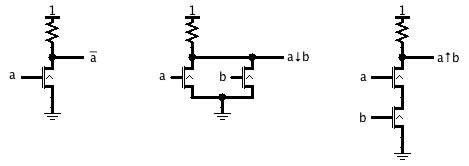
\includegraphics[width=!,height=!,scale=0.75]{graphics/NMOSgates.png}}

The \textsc{not} gate consists of a single transistor in the lower half:
the \nw{gate} on the left is connected to the input signal, $a$; the \nw{source}
at the bottom is connected to ground (0), and the \nw{drain} at the top is connected
to the output, $\overline{a}=\NOT a$, and a \nw{pull-up resistor} (the jagged line) whose
other end is at the high voltage level (1). When $a=0$ and the switch is open (so the
transistor effectively has infinite resistance), the output will be pulled high
(so $\overline{a}=1$). When $a=1$ and the switch is closed, the lower resistance
through the transistor will pull the output low (so $\overline{a}=0$).

The \textsc{nor} gate uses two transistors in parallel: if either $a$ or $b$ is
high, then the output ($a\downarrow b=\NOT(a\OR b)$) will be pulled low. Conversely, the \textsc{nand} gate
uses two transistors in series: both have to be closed (so $a=b=1$) for the
output ($a\uparrow b=\NOT(a\AND b)$) to be pulled to 0. Figure~\ref{fig:nandnorgates} shows the conventional
circuit symbols for \textsc{nand} and \textsc{nor} gates (note that the circle
on the output indicates negation, just like on the \textsc{not} gate; the
unnegated version of \textsc{not}, drawn as a simple triangle, is known as a
\nw{buffer}, because it copies its input to its output unchanged, after a short delay).

\fig
	{fig:nandnorgates}
	{The standard symbols for the \textsc{nand} and \textsc{nor} gates.}
	{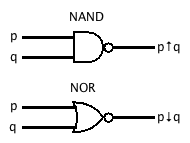
\includegraphics[width=!,height=!,scale=0.75]{graphics/NandNor.png}}

Those three gates are the simplest to implement with transistors. As we saw in the
exercises in Section~\ref{S-logic-1}, all other Boolean operators can be constructed
from \textsc{nand} alone, or \textsc{nor} alone. For example, an \textsc{and} gate is
a \textsc{nand} followed by a \textsc{not}, so it can be built out of three transistors;
an \textsc{or} gate also takes three, using a \textsc{nor} and a \textsc{not}.
In Section~\ref{sec:circsimp}, we will see another way to construct circuits using only \textsc{nand} gates.

\medskip

Given any compound proposition made from the operators
$\AND$, $\OR$, and $\NOT$, it is possible to build a logic
circuit\index{logic circuit!and compound propositions}
that computes the value of that proposition.\index{proposition!for a logic circuit}  The
proposition itself is a blueprint for the circuit.  As noted
in Section~\ref{S-logic-1}, every logical operator that we have 
encountered can be expressed in terms of $\AND$, $\OR$, and $\NOT$,
so in fact every compound proposition that we know how to write
can be computed by a logic circuit. 

Given a proposition constructed
from $\AND$, $\OR$, and $\NOT$ operators, it is
easy to build a circuit to compute it.  First, identify the main
operator in the proposition---the one whose value will be
computed \emph{last}.  Consider $(A\OR B)\AND\NOT(A\AND B)$.
This circuit has two input values, $A$ and $B$, which are represented
by wires coming into the circuit.  The circuit has an output wire
that represents the computed value of the proposition.
The main operator in $(A\OR B)\AND\NOT(A\AND B)$,
is the first~$\AND$, which computes the
value of the expression as a whole by combining the values
of the subexpressions $A\OR B$ and $\NOT(A\AND B)$.  This $\AND$
operator corresponds to an \textsc{and} gate in the circuit that
computes the final output of the circuit.

Once the main operator has been identified and represented as
a logic gate, you just have to build circuits to compute the
input or inputs to that operator.  In the  example,
the inputs to the main \textsc{and} gate come from two subcircuits.
One subcircuit computes the value of $A\OR B$ and the other
computes the value of $\NOT(A\AND B)$.  Building each subcircuit
is a separate problem, but smaller than the problem you started
with.  Eventually, you'll come to a gate whose input comes directly
from one of the input wires---$A$ or $B$ in this case---instead of
from a subcircuit.


\fig
   {F-buildlc}
   {Stages in the construction of a circuit that computes
    the compound proposition $(A\OR B)\AND\NOT(A\AND B)$.}
   {\scaledeps{4truein}{fig-1-4}}
   
   


\medbreak
   
So, every compound proposition is computed by a logic circuit
with one output wire.  Is the reverse true?  That is, given
a logic circuit with one output, is there a proposition that
expresses the value of the output in terms of the values of
the inputs?  Not quite.  When you wire together some logic
gates to make a circuit, there is nothing to stop you from
introducing feedback\index{feedback in circuits} loops.  A feedback loop occurs when
the output from a gate is connected---possibly through one
or more intermediate gates---back to an input of the same gate.
Figure~\ref{F-feedbacklc} shows an example of a circuit with
a feedback loop.
Feedback loops cannot be described by compound propositions,
basically because there is no place to start, no input to
associate with a propositional variable.  But feedback
loops are the only thing that can go wrong.  A logic circuit
that does not contain any feedback loops is called a
\nw{combinational logic circuit}.  Every combinational
logic circuit with just one output computes the value of
some compound proposition.  The propositional variables in
the compound proposition are just names associated with
the input wires of the circuit.  (Of course, if the circuit has
more than one output, you can simply use a different proposition
for each output.)  

\fig
   {F-feedbacklc}
   {This circuit contains a feedback loop, so it is not a
    combinational logic circuit.  The feedback loop includes
    the \textsc{and} gate and the \textsc{or} gate on the right.
    This circuit does not compute the value of a compound proposition.
    This circuit does, however, play an important role in computer
    memories, since it can be used to store a logical value.}
   {\scaledeps{4truein}{fig1-5}}

The key to understanding why this is true
is to note that each wire in the circuit---not just the final
output wire---represents the value of some proposition.  
Furthermore, once you know which proposition is represented by
each input wire to a gate, it's obvious what proposition is
represented by the output: You just combine the input propositions
with the appropriate $\AND$, $\OR$, or $\NOT$ operator, depending
on what type of gate it is.   To find
the proposition associated with the final output, you just have to
start from the inputs and move through the circuit, labeling the
output wire of each gate with the proposition that it represents.
Figure~\ref{F-labellc} illustrates this process.

\fig
    {F-labellc}
    {Finding the proposition whose value is computed by a
     combinational logic circuit.  Each wire in the circuit is
     labeled with the proposition that it represents.  The
     numbering of the labels shows one of the orders in which they 
     can be associated with the wires.  The circuit as a whole
     computes the value of $\NOT(A\AND B)\AND(B\OR\NOT C)$.}
    {\scaledeps{4truein}{fig1-6}}

\medbreak

A combinational circuit is one in which the output is entirely determined by the inputs---it is a pure function, with no dependence on state or time (apart from the initial time it takes the circuit to compute the output; see below). As such, its behavior is completely determined by a truth table; as we have seen, this means that it corresponds to a logical expression built up from the inputs and our basic operators.

When implementing a Boolean expression as a digital circuit, it is conventional to use a two-dimensional graphical representation of the circuit. This is partly because the circuit will eventually be laid out on a physical circuit board or semiconductor chip, and the relative locations of the gates and their interconnections will be important (although we will not go to this level of detail), but also because it can be easier to examine some of the properties and behavior of a circuit in a graphical form.

Another way to get this graphical representation is to use an \nw{expression tree}, which is a variation of the parse trees studied in Section~\ref{S-grammars-3}. For example, we may picture the expression $s=(a\OR b)\AND\NOT(a\AND b)$ as in Figure~\ref{fig:exprtree}.

\fig
	{fig:exprtree}
	{Expression tree for $s=(a\OR b)\AND\NOT(a\AND b)$}
	{\[ \setlength{\unitlength}{0.75pt}
\begin{picture}(120,140)
\put(10,40){\makebox(0,0){$a$}}
\put(50,40){\makebox(0,0){$b$}}
\put(30,70){\makebox(0,0){\textsc{or}}}
\put(10,45){\line(1,1){20}}
\put(50,45){\line(-1,1){20}}
\put(70,10){\makebox(0,0){$a$}}
\put(110,10){\makebox(0,0){$b$}}
\put(90,40){\makebox(0,0){\textsc{and}}}
\put(70,15){\line(1,1){20}}
\put(110,15){\line(-1,1){20}}
\put(90,70){\makebox(0,0){\textsc{not}}}
\put(90,45){\line(0,1){20}}
\put(60,100){\makebox(0,0){\textsc{and}}}
\put(30,75){\line(3,2){30}}
\put(90,75){\line(-3,2){30}}
\put(60,130){\makebox(0,0){$s$}}
\put(60,105){\line(0,1){20}}
\end{picture} \]}

Of course, we are usually interested in circuits that may have multiple outputs, so we may use a forest of expression trees. Figure~\ref{fig:exprforest} shows a forest for the same expression as above, along with the additional output $c$ given by $a\AND b$.

\fig
	{fig:exprforest}
	{Expression forest for $s=(a\OR b)\AND\NOT(a\AND b)$ and $c=a\AND b$}
	{\[ \setlength{\unitlength}{0.75pt}
\begin{picture}(200,140)
\put(10,40){\makebox(0,0){$a$}}
\put(50,40){\makebox(0,0){$b$}}
\put(30,70){\makebox(0,0){\textsc{or}}}
\put(10,45){\line(1,1){20}}
\put(50,45){\line(-1,1){20}}
\put(70,10){\makebox(0,0){$a$}}
\put(110,10){\makebox(0,0){$b$}}
\put(90,40){\makebox(0,0){\textsc{and}}}
\put(70,15){\line(1,1){20}}
\put(110,15){\line(-1,1){20}}
\put(90,70){\makebox(0,0){\textsc{not}}}
\put(90,45){\line(0,1){20}}
\put(60,100){\makebox(0,0){\textsc{and}}}
\put(30,75){\line(3,2){30}}
\put(90,75){\line(-3,2){30}}
\put(60,130){\makebox(0,0){$s$}}
\put(60,105){\line(0,1){20}}
\put(150,70){\makebox(0,0){$a$}}
\put(190,70){\makebox(0,0){$b$}}
\put(170,100){\makebox(0,0){\textsc{and}}}
\put(150,75){\line(1,1){20}}
\put(190,75){\line(-1,1){20}}
\put(170,130){\makebox(0,0){$c$}}
\put(170,105){\line(0,1){20}}
\end{picture} \]}

Upon doing this, we might notice that the subtree for $a\AND b$ is duplicated. It would be nice to share common parts of the circuit, thus giving us an expression DAG (\nw{directed acyclic graph}) instead of a tree or forest. One way to do this is shown in Figure~\ref{fig:exprdag1}.

\fig
	{fig:exprdag1}
	{Expression DAG for $s=(a\OR b)\AND\NOT(a\AND b)$ and $c=a\AND b$}
	{\[ \setlength{\unitlength}{0.75pt}
\begin{picture}(150,140)
\put(10,40){\makebox(0,0){$a$}}
\put(50,40){\makebox(0,0){$b$}}
\put(30,70){\makebox(0,0){\textsc{or}}}
\put(10,45){\line(1,1){20}}
\put(50,45){\line(-1,1){20}}
\put(100,10){\makebox(0,0){$a$}}
\put(140,10){\makebox(0,0){$b$}}
\put(120,40){\makebox(0,0){\textsc{and}}}
\put(100,15){\line(1,1){20}}
\put(140,15){\line(-1,1){20}}
\put(90,70){\makebox(0,0){\textsc{not}}}
\put(120,45){\line(-3,2){30}}
\put(60,100){\makebox(0,0){\textsc{and}}}
\put(30,75){\line(3,2){30}}
\put(90,75){\line(-3,2){30}}
\put(60,130){\makebox(0,0){$s$}}
\put(60,105){\line(0,1){20}}
\put(120,130){\makebox(0,0){$c$}}
\put(120,45){\line(0,1){80}}
\end{picture} \]}

We could also share the inputs rather than repeating them, as shown in Figure~\ref{fig:exprdag2}; this is still a DAG.

\fig
	{fig:exprdag2}
	{Expression DAG for $s=(a\OR b)\AND\NOT(a\AND b)$ and $c=a\AND b$, with shared inputs}
	{\[ \setlength{\unitlength}{0.75pt}
\begin{picture}(110,140)
\put(10,0){\makebox(0,0){$a$}}
\put(100,0){\makebox(0,0){$b$}}
\put(10,70){\makebox(0,0){\textsc{or}}}
\put(10,5){\line(0,1){60}}
\put(100,5){\line(-3,2){90}}
\put(100,40){\makebox(0,0){\textsc{and}}}
\put(10,5){\line(3,1){90}}
\put(100,5){\line(0,1){30}}
\put(70,70){\makebox(0,0){\textsc{not}}}
\put(100,45){\line(-3,2){30}}
\put(40,100){\makebox(0,0){\textsc{and}}}
\put(10,75){\line(3,2){30}}
\put(70,75){\line(-3,2){30}}
\put(40,130){\makebox(0,0){$s$}}
\put(40,105){\line(0,1){20}}
\put(100,130){\makebox(0,0){$c$}}
\put(100,45){\line(0,1){80}}
\end{picture} \]}

Finally, instead of using the words \textsc{and}, \textsc{or}, and \textsc{not}, we will use the corresponding circuit symbols; we also draw the DAG ``on its side,'' so that the flow from inputs to outputs is left-to-right. The final result is a circuit diagram such as Figure~\ref{fig:exprcircuit}.

\fig
	{fig:exprcircuit}
	{Circuit diagram for $s=(a\OR b)\AND\NOT(a\AND b)$ and $c=a\AND b$}
	{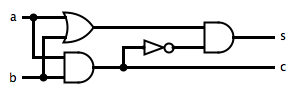
\includegraphics[width=!,height=!,scale=0.75]{graphics/HalfAdder.png}}

It is important to realize, though, that this is just another presentation of the logical expressions we started with. Any set of Boolean expressions may be drawn this way, and any circuit where all of the information flows from left to right may be read as a set of expressions.

In addition to visualizing the layout of gates in a digital circuit, a circuit diagram may be used to ``trace'' its operation on particular inputs. For example, Figure~\ref{fig:exprcircuit11} is our example circuit annotated with 0/1 logic values on each wire, to trace its behavior when both inputs $a$ and $b$ are 1. Since the logic values flow from left to right, the output of each successive gate may be determined from its inputs. By tracing each combination of inputs, we may construct a truth table corresponding to the circuit; the result is
\[ \begin{array}{cc|cc}
a  & b  & c & s\\ \hline
0 & 0 & 0 & 0\\
0 & 1 & 0 & 1\\
1 & 0 & 0 & 1\\
1 & 1 & 1 & 0
\end{array} \]

\fig
	{fig:exprcircuit11}
	{Annotated diagram for $s=(a\OR b)\AND\NOT(a\AND b)$ and $c=a\AND b$ when $a=1$ and $b=1$}
	{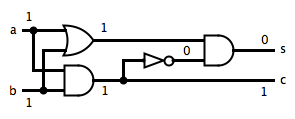
\includegraphics[width=!,height=!,scale=0.75]{graphics/HalfAdder11.png}}

\medbreak
   
So, compound propositions correspond naturally with combinational
logic circuits.  But we have still not quite settled the question
of just how powerful these circuits and propositions are.
We've looked at a number of logical operators and noted that they
can all be expressed in terms of $\AND$, $\OR$, and~$\NOT$.
But might there be other operators that cannot be so expressed?
Equivalently, might there be other types of logic gates---possibly
with some large number of inputs---whose
computations cannot be duplicated with \textsc{and}, \textsc{or}, and
\textsc{not} gates?   Any logical operator or logic gate computes
a value for each possible combination of logical values of its inputs.
We could always make a truth table showing the output for each 
possible combination of inputs.  As it turns out, given \emph{any} such
truth table,\index{truth table!and logic circuits} it is possible to find a proposition, containing only
the $\AND$, $\OR$, and~$\NOT$ operators, whose value for each combination
of inputs is given precisely by that table.    

To see why this is true, it is useful to introduce a particular type
of compound proposition.  Define a \nw{simple term} to be either
a propositional variable or the negation of a propositional variable.
A conjunction of simple terms would then consist of one or more
simple terms put together with $\AND$ operators.  (A ``conjunction of
one simple term'' is just a single simple term by itself.  This might
not make grammatical sense, but it's the way mathematicians think.)
Some examples of conjunctions of simple terms would be
$p\AND q$, $p$, $\NOT q$, and $p\AND\NOT r\AND \NOT w\AND s\AND t$.
Finally, we can take one or more such conjunctions and join them
into a ``disjunction of conjunctions of simple terms.''  This is the
type of compound proposition we need.  We can avoid some redundancy
by assuming that no propositional variable occurs more than once
in a single conjunction (since $p\AND p$ can be replaced by $p$,
and if $p$ and $\NOT p$ both occur in a conjunction, then the value
of the conjuction is false, and it can be eliminated.)  We can also
assume that the same conjunction does not occur twice in the
disjunction.
\begin{definition}\label{D-DNF}
A compound proposition is said to be in \nw{disjunctive normal form},
or DNF, if it is a disjunction of conjunctions of simple terms,
and if, furthermore, each propositional variable occurs at most once
in each conjunction and each conjunction occurs at most once in the
disjunction.
\end{definition}
Using $p$, $q$, $r$, $s$, $A$, and $B$ as propositional variables,
here are a few examples of propositions that are in disjunctive
normal form:
\[
\begin{array}{c}
(p\AND q\AND r)\OR(p\AND\NOT q\AND r\AND s)\OR(\NOT p\AND\NOT q)\\
(p\AND \NOT q)\\
(A\AND \NOT B)\OR(\NOT A\AND B)\\
p\OR(\NOT p\AND q)\OR(\NOT p\AND\NOT q\AND r)\OR(\NOT p\AND\NOT q\AND\NOT r\AND w)\\
\end{array}
\]
Propositions in DNF are just what we need to deal with input/output
tables of the type that we have been discussing.  Any such table
can be computed by a proposition in disjunctive normal form.
It follows that it is  possible to build a circuit\index{logic circuit!for an input/output table} to compute that 
table using only \textsc{and}, \textsc{or}, and \textsc{not} gates.

\begin{theorem}\label{T-DNF}
Consider a table that lists a logical output value for every
combination of values of several propositional variables.
Assume that at least one of the output values is true.
Then there is a proposition containing those variables such that
the value of the proposition for each possible combination of
the values of the variables is precisely the value specified
in the table.  It is possible to choose the proposition to
be in disjunctive normal form.\index{proposition!equivalent to one in DNF}
\end{theorem}
\begin{proof}
Consider any row in the table for which the output value is $\T$.
Form a conjunction of simple terms as follows: For each variable, $p$,
whose value is $\T$ in that row, include $p$ itself in the conjunction;
for each variable, $q$, whose value is $\F$ in the row, include
$\NOT q$ in the conjunction.  The value of this conjunction is
$\T$ for the combination of variable values given in that row
of the table, since each of the terms in the conjuction is true
for that combination of variables.  Furthermore, for any \emph{other}
possible combination of variable values, the value of the conjunction
will be $\F$, since at least one of the simple terms in the 
conjunction will be false.

Take the disjunction of all such conjunctions constructed in this
way, for each row in the table where the output value is true.
This disjunction has the value $\T$ if and only if one of
the conjunctions that make it up has the value~$\T$---and that is
precisely when the output value specified by the table is~$\T$.
So, this disjunction of conjunctions satisfies the requirements of
the theorem.
\end{proof} 

As an example, consider the table in Figure~\ref{F-inputoutput1}.
This table specifies a desired output value for each possible
combination of values for the propositional variables $p$,
$q$, and $r$.  Look at the second row of the table, where
the output value is true.  According to the proof of the theorem,
this row corresponds to the conjunction $(\NOT p\AND\NOT q\AND r)$.
This conjunction is true when $p$ is false, $q$ is false,
and $r$ is true; in all other cases it is false, since in any other
case at least one of the terms $\NOT p$, $\NOT q$, or $r$~is
false.  The other two rows where the output is true give
two more conjunctions.  The three conjunctions are combined
to produce the  DNF proposition $(\NOT p\AND\NOT q\AND r) \OR
(\NOT p\AND q\AND r) \OR (p\AND q\AND r)$.  This proposition
computes all the output values specified in the table.
Using this proposition as a blueprint, we get a logic circuit
whose outputs match those given in the table.

\fig
   {F-inputoutput1}
   {An input/output table specifying a desired output for each
    combination of values of the propositional variables $p$,
    $q$, and $r$.  Each row where the output is $\T$ corresponds to
    a conjunction, shown next to that row in the table.  The
    disjunction of these conjunctions is a proposition whose
    output values are precisely those specified by the table.}
   {\begin{tabular}{|c|c|c||c|l}
       \cline{1-4}
       \strut $p$&  $q$&  $r$& output& \\
       \cline{1-4}
       \strut $\F$& $\F$& $\F$& $\F$& \\
       \cline{1-4}
       \strut $\F$& $\F$& $\T$& $\T$& $(\NOT p\AND\NOT q\AND r)$\\
       \cline{1-4}
       \strut $\F$& $\T$& $\F$& $\F$& \\
       \cline{1-4}
       \strut $\F$& $\T$& $\T$& $\T$& $(\NOT p\AND q\AND r)$\\
       \cline{1-4}
       \strut $\T$& $\F$& $\F$& $\F$& \\
       \cline{1-4}
       \strut $\T$& $\F$& $\T$& $\F$& \\
       \cline{1-4}
       \strut $\T$& $\T$& $\F$& $\F$& \\
       \cline{1-4}
       \strut $\T$& $\T$& $\T$& $\T$& $p\AND q\AND r$\\
       \cline{1-4}
    \end{tabular}
   }
   
\medbreak

Now, given any combinational logic circuit, there are many
other circuits that have the same input/output behavior. 
When two circuits have the same input/output table,
the compound propositions associated with
the two circuits are logically equivalent.  To put this another
way, propositions that are logically equivalent produce circuits
that have the same input/output behavior.  As a practical matter,
we will usually prefer the circuit that is simpler.  The
correspondence between circuits and propositions allows us
to apply Boolean algebra\index{Boolean algebra!and logic circuits}
to the simplification of circuits.\index{logic circuit!simplifying}

For example, consider the DNF proposition corresponding to the
table in Figure~\ref{F-inputoutput1}.  In $(\NOT p\AND\NOT q\AND r) \OR
(\NOT p\AND q\AND r) \OR (p\AND q\AND r)$, we can factor $(q\AND r)$
from the last two terms, giving $(\NOT p\AND\NOT q\AND r) \OR
((\NOT p\OR p) \AND (q\AND r))$.  Since $\NOT p\OR p\equiv\T$,
and $\T\AND Q\equiv Q$ for any proposition $Q$,
this can be simplified to $(\NOT p\AND\NOT q\AND r) \OR (q\AND r)$.
Again, we can apply the distributive law to this to factor
out an $r$, giving $((\NOT p\AND \NOT q)\OR q)\AND r)$.
This compound proposition is logically equivalent to the one we
started with, but implementing it in a circuit
requires only five logic gates, instead of the
ten required by the original proposition.\footnote{No, I didn't
count wrong.  There are eleven logical operators in the original
expression, but you can get by with ten gates in the circuit:
Use a single \textsc{not} gate to compute $\NOT p$, and connect
the output of that gate to two different \textsc{and} gates.
Reusing the output of a logic gate is an obvious way to simplify
circuits that does not correspond to any operation on propositions.}

If you start with a circuit instead of a proposition, it is
often possible to find the associated proposition, simplify it
using Boolean algebra, and use the simplified proposition to
build an equivalent circuit that is simpler than the original.


\medbreak

All this explains nicely the relationship between logic
and circuits, but it doesn't explain why logic circuits
should be used in computers in the first place.  Part of
the explanation is found in the fact that computers use binary
numbers.\index{binary number}  A binary number is a string of zeros and ones.
Binary numbers are easy to represent in an electronic device
like a computer:  Each position in the number corresponds to
a wire. When the wire is on, it represents one; when the
wire is off, it represents zero.  When we are thinking in terms
of logic, the same states of the wire represent true and false,
but either representation is just an interpretation of the
reality, which is a wire that is on or off.  The question is
whether the interpretation is fruitful.

Once wires are thought of as representing zeros and ones,
we can build circuits to do computations with binary numbers.
Which computations?  Any that we want!  If we know
what the answer should be for each combination of inputs,
then by Theorem~\ref{T-DNF} we can build a circuit to compute
that answer.  Of course, the procedure described in that 
theorem is only practical for small circuits, but small
circuits can be used as building blocks to make all the
calculating circuits in a computer.

\fig
   {F-inputoutput2}
   {Input/output tables for the addition of three binary 
    digits, $A$, $B$, and $C$.}
   {\mbox{
      \begin{tabular}{|c|c|c||c|}
         \hline
         \strut $A$& $B$& $C$& output\\
         \hline
         \strut 0& 0& 0& 0 \\
         0& 0& 1& 1 \\
         0& 1& 0& 1 \\
         0& 1& 1& 0 \\
         1& 0& 0& 1 \\
         1& 0& 1& 0 \\
         1& 1& 0& 0 \\
         1& 1& 1& 1 \\
         \hline
      \end{tabular}
    \qquad
      \begin{tabular}{|c|c|c||c|}
         \hline
         \strut $A$& $B$& $C$& output\\
         \hline
         \strut 0& 0& 0& 0 \\
         0& 0& 1& 0 \\
         0& 1& 0& 0 \\
         0& 1& 1& 1 \\
         1& 0& 0& 0 \\
         1& 0& 1& 1 \\
         1& 1& 0& 1 \\
         1& 1& 1& 1 \\
      \hline
      \end{tabular}
    }
   }

For example, let's look at binary addition.\index{addition, binary}  To add two ordinary,
decimal numbers, you line them up one on top of the other,
and add the digits in each column.  In each column, there might
also be a carry from the previous column.  To add up a
column, you only need to remember a small number of rules,
such as $7+6+1=14$ and $3+5+0=8$.  For binary addition, it's
even easier, since the only digits are 0 and~1.  There are
only eight rules:
\begin{align*}
0+0+0&=00 & 1+0+0&=01\\
0+0+1&=01 & 1+0+1&=10\\
0+1+0&=01 & 1+1+0&=10\\
0+1+1&=10 & 1+1+1&=11\\
\end{align*}
Here, I've written each sum using two digits.  In a multi-column
addition, one of these digits is carried over to the next column.
Here, we have a calculation that has three inputs and two outputs.
We can make an input/output table for each of the two outputs.  The
tables are shown in Figure~\ref{F-inputoutput2}.  We know that these
tables can be implemented as combinational circuits, so we know that
circuits can add binary numbers.  To add multi-digit binary numbers,
we just need one copy of the basic addition circuit for each column
in the sum.





\begin{exercises}

\problem Using only \textsc{and}, \textsc{or}, and \textsc{not} gates,
draw circuits that compute the value of each of the propositions
$A\IMP B$, $A\IFF B$, and $A\XOR B$.

\problem For each of the following propositions, find a combinational
logic circuit that computes that proposition:
\pparts{
       A\AND (B\OR \NOT C)      & (p\AND q)\AND\NOT(p\AND\NOT q) \cr
       (p\OR q\OR r)\AND (\NOT p\OR \NOT q\OR \NOT r)
                                & \NOT(A\AND (B\OR C)) \OR (B\AND \NOT A)\cr
}

\problem Find the compound proposition computed by each of the
following circuits:
\medskip

\centerline{\qquad\scaledeps{3.6truein}{fig-1-label}}

\problem This section describes a method for finding the compound
proposition computed by any combinational logic circuit.  This method
fails if you try to apply it to a circuit that contains a feedback loop.
What goes wrong?  Give an example.

\problem Show that every compound proposition which is not a contradiction
is equivalent to a proposition in disjunctive normal form.  (Note: We can
eliminate the restriction that the compound proposition is not a
contradiction by agreeing that ``$\F$'' counts as a proposition in
disjunctive normal form.  $\F$~is logically equivalent to any contradiction.)

\problem\label{ex:CNF}A proposition in \nw{conjunctive normal form} (CNF) is
a conjunction of disjunctions of simple terms (with the proviso, as 
in the definition of DNF that a single item counts as a conjunction
or disjunction).  Show that every 
compound proposition which is not a tautology is logically equivalent
to a compound proposition in conjunctive normal form.  (Hint:
What happens if you take the negation of a DNF proposition and
apply DeMorgan's Laws?)

\problem Use the laws of Boolean algebra to simplify each of the
following circuits:
\medskip

\rightline{\scaledeps{4.2 true in}{fig-1-simplify}}


\problem Design circuits to implement the input/output tables
for addition, as given in Figure~\ref{F-inputoutput2}.  Try to
make your circuits as simple as possible.  (The circuits that are
used in real computers for this purpose are more simplified than
the ones you will probably come up with, but the general approach
of using logic to design computer circuits is valid.)

\end{exercises}

\subsection{Circuit Simplification}\label{sec:circsimp}
As noted above, a physical circuit does have some dependence on time, since each device in the circuit requires a non-zero time to respond to a change in its inputs. A more precise model needs to take these delays into account---a circuit is modeled by a Boolean expression \emph{plus} a set of delay factors (other cost measures may also be important: power consumption, heat production, area occupied, \textit{etc.}, but we will focus on the delay issue here). We will make the simplifying assumption that all gates have the same delay time, so we will measure the total delay of a circuit in terms of the number of gate delays required before the output values accurately reflect a change to the input values.

Given a combinational circuit, we may compute the delay, also known as the \nw{span}, by finding the number of gates on the longest path (the \nw{critical path}) from an input to an output. For example, the circuit in Figure~\ref{F-labellc} has a span of three gate delays, with the critical path passing either through the \textsc{and}, \textsc{not}, \textsc{and} sequence along the top, or through the \textsc{not}, \textsc{or}, \textsc{and} along the bottom. Note that this is a conservative estimate of the delay required, although for certain inputs the output may become stable sooner---for example, if the $B$ input changes from 0 to 1
while $A$ is 0, then after one gate delay the output of the \textsc{or} will become 1; since the output of the upper \textsc{not} was already 1 in this case (why?), the final output will settle at 1 after only two gate delays. However, other combinations of inputs may well take the entire three gate delays to correctly determine the value of the output.

One approach to reducing the delay of a circuit is to use the disjunctive normal form, also known as the \nw{sum-of-products} (see Definition~\ref{D-DNF}). Since an expression in DNF is the \textsc{or} of a collection of terms which are the \textsc{and} of some number of simple terms, and a simple term is either an input or a negated input, the corresponding circuit can be constructed in three layers:
\begin{center}
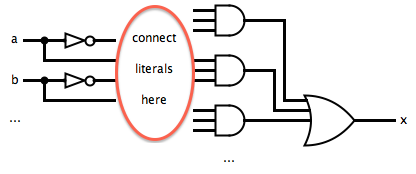
\includegraphics[width=!,height=!,scale=0.75]{graphics/DNFlayers.png}
\end{center}

An interesting property of the sum-of-products representation falls out of the De Morgan laws. Since $(a\AND b)\OR(c\AND d)=\NOT(\NOT(a\AND b)\AND\NOT(c\AND d))=(a\uparrow b)\uparrow(c\uparrow d)$, the two layers of \textsc{and} and \textsc{or} gates may be replaced entirely with \textsc{nand} gates to get an equivalent circuit!
\begin{center}
\includegraphics[width=!,height=!,scale=0.75]{graphics/DNFlayersNand.png}
\end{center}

Unfortunately, this does not mean that any Boolean expression can be computed by a circuit with only three gate delays. One problem comes when we need \textsc{and} and \textsc{or} gates (or \textsc{nand} gates) with more than two inputs---in general, with $n$ input variables, there may be \textsc{and} gates that need $n$ inputs, and there could be on the order of $2^n$ gates in the \textsc{and} level, requiring an \textsc{or} gate with that many input lines. We will see in the next section how to build gates with a larger number of inputs out of gates with just two inputs.

Another problem with DNF comes if we use the full DNF expression extracted from a truth table.
If we use Theorem~\ref{T-DNF} to produce an expression from the truth table for the implication $p\rightarrow q$, we will get $(\NOT p\AND\NOT q)\OR(\NOT p\AND q)\OR(p\AND q)$. We may use Boolean algebra identities to find an equivalent DNF expression, $\NOT p\OR q$ (which only needs two gate delays, since the \textsc{and} layer disappears). There are general techniques for finding simpler DNF expressions such as this; we will look at a straightforward technique called a \textit{Karnaugh map}, although for computer implementation the related Quine-McCluskey algorithm is better (and for large numbers of input variables a heuristic approach is necessary).

A Karnaugh map is a way of visualizing entries in a truth table so that adjacent entries only differ on the value of one input variable. For example, the entry for $\NOT p\AND q$ will be next to the entry for $p\AND q$. If adjacent entries each contain 1, meaning that those terms would participate in the full DNF expression, then they may be replaced by a single term with just the variables that are the same: in the example, this corresponds to the simplification $(\NOT p\AND q)\OR(p\AND q)=(\NOT p\OR p)\AND q=\T\AND q=q$.

For two input variables, a Karnaugh map is a $2\times 2$ array:
\[ \begin{array}{r|cc}
& \NOT{q} & q\\ \hline
\NOT{p} & x_{00} & x_{01}\\
p & x_{10} & x_{11}
\end{array} \]
This is just a compact rearrangement of the truth table:
\[ \begin{array}{cc|c}
p & q & x\\ \hline
0 & 0 & x_{00}\\
0 & 1 & x_{01}\\
1 & 0 & x_{10}\\
1 & 1 & x_{11}
\end{array} \]
However, note that the adjacent cell condition is true: horizontally adjacent cells only differ on $q$, while vertically adjacent cells only differ on $p$.

Once we have laid out the Karnaugh map, a simplified expression may be read off by finding a way to cover all of the 1's in the map with ``implicants.'' An implicant is a rectangle whose side lengths are a power of 2; it corresponds to finding a collection of adjacent cells in the map (all of which contain 1) that all agree on some of the input literals and that collectively include all combinations (negated or not) of the other input variables. The resulting term for an implicant is just the product of the common literals among all the cells covered by the implicant.

On a $2\times 2$ map, the only implicants are individual cells ($1\times 1$), a row ($1\times 2$), a column ($2\times 1$), or the entire map ($2\times 2$). The cells correspond to terms such as $p\AND\NOT{q}$, the rows are either $\NOT{p}$ or $p$, the columns are either $\NOT{q}$ or $q$, and the entire map is $1$ (the empty product). To get the simplest expression, we want to take the fewest number of the largest possible implicants that between them cover all of the 1's in the map. Implicants may overlap, as long as all of (and only) the 1's are covered by at least one implicant.

Here is the example again. First the truth table for $p\rightarrow q$:
\[ \begin{array}{cc|c}
p & q & x\\ \hline
0 & 0 & 1\\
0 & 1 & 1\\
1 & 0 & 0\\
1 & 1 & 1
\end{array} \]
As a Karnaugh map, this is:
\[ \begin{array}{r|cc}
& \NOT{q} & q\\ \hline
\NOT{p} & 1 & 1\\
p & 0 & 1
\end{array} \]
The best way to cover this map with implicants is to take the first row and the second column. That gives the simplified terms $\NOT{p}$ and $q$, so the final simplified expression is $\NOT{p}\OR q$. Here is the map with the implicants outlined:
\[ \begin{array}{r|cc}
& \NOT{q} & q\\ \hline
\NOT{p} & \tikzmark{left1}1 & \tikzmark{left2}1\tikzmark{right1}\\
p & 0 & 1\tikzmark{right2}
\end{array}
\DrawBox[blue]{left1}{right1}
\DrawBox[red]{left2}{right2} \]

A Karnaugh map can also work with three or four input variables, producing either a $2\times 4$ or a $4\times 4$ array. The same procedure applies, with three complications:
\begin{enumerate}
\item To satisfy the adjacent cell condition, successive rows or columns must change only one variable at a time: for example, the rows might be labelled in order $\NOT{p}\AND\NOT{q}$, $\NOT{p}\AND q$, $p\AND q$, and $p\NOT{q}$;
\item Implicants may be 1, 2, or 4 rows tall by 1, 2, or 4 columns wide; and
\item Implicants may ``wrap around'' from one side of the map to the other.
\end{enumerate}
For example, on a $4\times 4$ map, one possible implicant is the middle two rows; another is the leftmost and rightmost columns (wrapping horizontally); a third is the $2\times 2$ block consisting of the middle two elements of the top row and the middle two elements of the bottom row (wrapping vertically); a final example is the last two elements of the third row. See Figure~\ref{fig:KarnaughImplicants} for these examples.

\begin{figure}
Middle two rows ($q$):
\[ \begin{array}{r|cccc}
& \NOT{r}\AND\NOT{s} & \NOT{r}\AND s & r\AND s & r\AND\NOT{s}\\ \hline
\NOT{p}\AND\NOT{q} & & & & \\
\NOT{p}\AND q & \tikzmark{left1}1 & 1 & 1 & 1\\
p\AND q & 1 & 1 & 1 & 1\tikzmark{right1}\\
p\AND\NOT{q} & & & &
\end{array}
\DrawBox[blue]{left1}{right1} \]

Leftmost and rightmost columns ($\NOT{s}$):
\[ \begin{array}{r|cccc}
& \NOT{r}\AND\NOT{s} & \NOT{r}\AND s & r\AND s & r\AND\NOT{s}\\ \hline
\NOT{p}\AND\NOT{q} & \tikzmark{left1}1 & & & \tikzmark{left2}1\\
\NOT{p}\AND q & 1 & & & 1\\
p\AND q & 1 & & & 1\\
p\AND\NOT{q} & 1\tikzmark{right1} & & & 1\tikzmark{right2}
\end{array}
\DrawBoxW[blue]{left1}{right1}
\DrawBoxE[blue]{left2}{right2} \]

Middle elements of top and bottom rows ($\NOT{q}s$):
\[ \begin{array}{r|cccc}
& \NOT{r}\AND\NOT{s} & \NOT{r}\AND s & r\AND s & r\AND\NOT{s}\\ \hline
\NOT{p}\AND\NOT{q} & & \tikzmark{left1}1 & 1\tikzmark{right1} & \\
\NOT{p}\AND q & & & &\\
p\AND q & & & &\\
p\AND\NOT{q} & & \tikzmark{left2}1 & 1\tikzmark{right2} &
\end{array}
\DrawBoxN[blue]{left1}{right1}
\DrawBoxS[blue]{left2}{right2} \]

Last two elements of the third row ($pqr$):
\[ \begin{array}{r|cccc}
& \NOT{r}\AND\NOT{s} & \NOT{r}\AND s & r\AND s & r\AND\NOT{s}\\ \hline
\NOT{p}\AND\NOT{q} & & & & \\
\NOT{p}\AND q & & & &\\
p\AND q & & & \tikzmark{left1}1 & 1\tikzmark{right1}\\
p\AND\NOT{q} & & & &
\end{array}
\DrawBox[blue]{left1}{right1} \]
\caption{Some examples of Karnaugh map implicants}
\label{fig:KarnaughImplicants}
\end{figure}

A Karnaugh map also allows us to find simple circuits in the case that some combinations of inputs will never occur, so that we do not care what the output is in those rows of the truth table. By entering a \nw{don't care} value, such as X, in the map, we have the freedom to either ignore or include those cells when covering the map with implicants; by including a cell with an X along with a group of 1's, we might be able to construct a larger (and hence simpler) implicant.

For example, suppose we have the following truth table for a four-variable Boolean expression (this represents the inputs that are binary numbers less than ten and divisible by three):
\[ \begin{array}{cccc|c}
p & q & r & s & x\\ \hline
0 & 0 & 0 & 0 & 1\\
0 & 0 & 0 & 1 & 0\\
0 & 0 & 1 & 0 & 0\\
0 & 0 & 1 & 1 & 1\\
0 & 1 & 0 & 0 & 0\\
0 & 1 & 0 & 1 & 0\\
0 & 1 & 1 & 0 & 1\\
0 & 1 & 1 & 1 & 0\\
1 & 0 & 0 & 0 & 0\\
1 & 0 & 0 & 1 & 1\\
1 & 0 & 1 & 0 & X\\
1 & 0 & 1 & 1 & X\\
1 & 1 & 0 & 0 & X\\
1 & 1 & 0 & 1 & X\\
1 & 1 & 1 & 0 & X\\
1 & 1 & 1 & 1 & X
\end{array} \]
As a Karnaugh map, this is:
\[ \begin{array}{r|cccc}
& \NOT{r}\AND\NOT{s} & \NOT{r}\AND s & r\AND s & r\AND\NOT{s}\\ \hline
\NOT{p}\AND\NOT{q} & 1 & 0 & 1 & 0\\
\NOT{p}\AND q & 0 & 0 & 0 & 1\\
p\AND q & X & X & X & X\\
p\AND\NOT{q} & 0 & 1 & X & X
\end{array} \]
The 1's, plus some of the X's, may be covered by four implicants: $\NOT{p}\AND\NOT{q}\AND\NOT{r}\AND\NOT{s}$, $\NOT{q}\AND r\AND s$, $q\AND r\AND\NOT{s}$, and $p\AND s$. Note that the second implicant wraps around from the third cell on the top row to the third cell (with an X, which is also covered by the $p\AND s$ implicant) on the bottom row; if it were just the 1 on the top row, then the term would be $\NOT{p}\AND\NOT{q}\AND r\AND s$, which is not as simple. Here are the cells that end up being covered:
\[ \begin{array}{r|cccc}
& \NOT{r}\AND\NOT{s} & \NOT{r}\AND s & r\AND s & r\AND\NOT{s}\\ \hline
\NOT{p}\AND\NOT{q} & \tikzmark{left1}1\tikzmark{right1} & 0 & \tikzmark{left2a}1\tikzmark{right2a} & 0\\
\NOT{p}\AND q & 0 & 0 & 0 & \tikzmark{left3}1\\
p\AND q & X & \tikzmark{left4}X & X & X\tikzmark{right3}\\
p\AND\NOT{q} & 0 & 1 & \tikzmark{left2b}X\tikzmark{right2b}\tikzmark{right4} & X
\end{array}
\DrawBox[blue]{left1}{right1}
\DrawBoxN[red,rounded corners=3pt]{left2a}{right2a}
\DrawBoxS[red,rounded corners=3pt]{left2b}{right2b}
\DrawBox[green]{left3}{right3}
\DrawBox[purple]{left4}{right4} \]
Therefore, the simplified expression is $(\NOT{p}\AND\NOT{q}\AND\NOT{r}\AND\NOT{s})\OR(\NOT{q}\AND r\AND s)\OR(q\AND r\AND\NOT{s})\OR(p\AND s)$. This may be computed by the following circuit:
\begin{center}
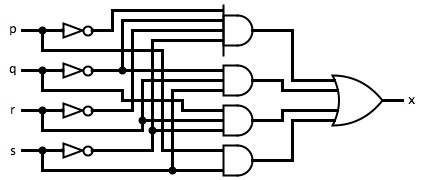
\includegraphics[width=!,height=!,scale=0.75]{graphics/KarnaughExample.png}
\end{center}
In the next section, we will see how to implement this with a total delay of 5, using only two-input \textsc{and} and \textsc{or} gates.

The final difficulty with building low-delay circuits from DNF expressions is that, even with the simplification provided by something like a Karnaugh map, many Boolean functions lead to an exponential blowup when expressed in DNF. In the worst case, an expression with $n$ input variables may require $O(2^n)$ terms in a sum-of-product representation---consider the case of a Karnaugh map where the 1's are in a checkerboard arrangement, so that none are adjacent. When $n$ is large enough, it might not even be practical to consider the truth table at all; for example, a circuit that can add two 32-bit numbers requires 64 input lines, which would lead to a truth table with $2^{64}\approx 10^{19}$ entries. The next section will also discuss approaches to this kind of problem.

\begin{exercises}
\problem For each of the following Boolean expressions, compute the total delay of the direct translation of the expression into a circuit.
\ppart $\NOT{(\NOT{p}\OR q)}\OR(\NOT{\NOT{q}}\OR\NOT{p})$
\ppart $(\NOT(\NOT{r}\AND p)\OR\NOT{q})\AND(\NOT(\NOT{r}\AND q)\OR\NOT{p})$
\ppart $(((p\OR q)\AND(q\OR r))\AND(r\OR s))\AND(((p\OR r)\AND(q\OR s))\AND(p\OR s))$

\problem For each of the expressions in the previous problem, use a Karnaugh map to find an equivalent sum-of-products expression, and draw the resulting circuit.

\problem Suppose we want to build a counter that cycles through the numbers 0, 1, 2, 3, 4, and back to 0. One element of this counter will be a circuit that takes the current number, expressed in binary, and outputs the next number. Here is the truth table for this function, with three inputs ($a$, $b$, and $c$) and three outputs ($x$, $y$, and $z$):
\[ \begin{array}{ccc|ccc}
a & b & c & x & y & z\\ \hline
0 & 0 & 0 & 0 & 0 & 1\\
0 & 0 & 1 & 0 & 1 & 0\\
0 & 1 & 0 & 0 & 1 & 1\\
0 & 1 & 1 & 1 & 0 & 0\\
1 & 0 & 0 & 0 & 0 & 0\\
1 & 0 & 1 & X & X & X\\
1 & 1 & 0 & X & X & X\\
1 & 1 & 1 & X & X & X\\
\end{array} \]
Since the counter should never reach numbers 5, 6, or 7, we do not care about the output when $abc$ is 101, 110, or 111. Use Karnaugh maps to find a simple circuit for this function.

\problem\label{ex:BCD}In binary-coded decimal (BCD), four bits are used to represent the numbers 0 (0000) through 9 (1001); the other six bit patterns (1010 through 1111) are unused. BCD is often used in circuits where decimal numbers need to be displayed; a common device for doing so is the \nw{seven-segment display}. Using only seven elements (for example, light-emitting diodes), we may form a reasonable approximation of all the digits 0--9: \textifsym{0123456789}. Construct a truth table with four inputs and seven outputs showing how to produce these characters from input in BCD (be sure to include a diagram indicating which output column corresponds to which display element). Use Karnaugh maps to design a relatively simple circuit that implements a seven-segment decoder.

\problem Exercise~\ref{ex:CNF} of Section~\ref{S-logic-3} examines conjunctive normal form (CNF), the dual of DNF. Explore what kind of circuits result from CNF, and how to extract a simplified CNF expression from a Karnaugh map \textit{(Hint: look at blocks of 0's.)}.

\end{exercises}

\subsection{Common Circuit Components}
Just as a complicated piece of software is never written from scratch entirely from the most basic program statements, a complicated hardware design is not approached purely at the gate level. Where a programmer will break the task into a hierarchy of objects and functions, relying on familiar idioms and existing code from program libraries to avoid reinventing the wheel, a hardware designer will use a hierarchy of functional blocks, relying on familiar patterns and existing libraries of subcircuits.

We have already seen one of these common components---the sample circuit in Figure~\ref{fig:exprcircuit} is known as the \nw{half adder}. If $a$ and $b$ represent one-bit binary numbers, then $s$ is their one-bit sum and $c$ is the carry into the next bit. For example, when $a$ and $b$ are both 1, $s$ is 0 and $c$ is 1; in binary, this says $1+1=10$. We may represent this block in a circuit diagram with an appropriately named box:
\begin{center}
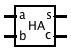
\includegraphics[width=!,height=!,scale=0.75]{graphics/HalfAdderSymbol.png}
\end{center}
It is called a half adder because, when you are adding multiple columns of bits, it only does half the work: it adds the two bits for a column, but it doesn't add in the carry from the next smaller column. A \nw{full adder} takes three inputs: $a$ and $b$, plus the incoming carry, $c_\textit{\scriptsize in}$. The outputs are $s$, the sum that stays in the column, plus the outgoing carry to the next column, $c_\textit{\scriptsize out}$. We may build a full adder out of two half adders by first adding $a$ to $b$, then adding $c_\textit{\scriptsize in}$; since the highest total in a full adder is three (11), we will never have a carry out of more than one of the half adders, so the resulting $c_\textit{\scriptsize out}$ is just the \textsc{or} of the two half adder carries. Here is the circuit with its block symbol and its truth table:
\[
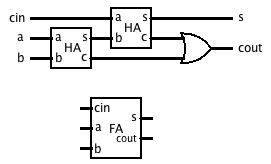
\includegraphics[width=!,height=!,scale=0.75]{graphics/FullAdder.png}\hspace{1cm}
\begin{array}[b]{ccl|rc}
a & b & c_\textit{\scriptsize in} & c_\textit{\scriptsize out} & s\\ \hline
0 & 0 & 0 & 0 & 0\\
0 & 0 & 1 & 0 & 1\\
0 & 1 & 0 & 0 & 1\\
0 & 1 & 1 & 1 & 0\\
1 & 0 & 0 & 0 & 1\\
1 & 0 & 1 & 1 & 0\\
1 & 1 & 0 & 1 & 0\\
1 & 1 & 1 & 1 & 1
\end{array}
\]

Given a full adder, we may construct multiple-bit adders by \nw{cascading} them, with the carry from each column feeding into the next. Here, for example, is a four-bit adder; the inputs are $a_3a_2a_1a_0$ and $b_3b_2b_1b_0$, plus an incoming carry $c_\textit{\scriptsize in}$ to column 0 (the one's column), and the outputs are $s_3s_2s_1s_0$, plus a carry from column 3 (the eight's column), $c_\textit{\scriptsize out}$:
\begin{center}
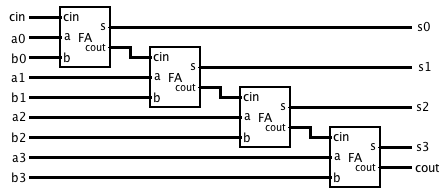
\includegraphics[width=!,height=!,scale=0.75]{graphics/4BitAdder.png}
\end{center}
Exercise~\ref{ex:cascade} explores whether this is a good design.

A common pattern in logic circuits is to use the \textsc{and} gate to ``enable'' (or disable) some signal. For example, in the half adder, the sum output, $s$, is true when one of the inputs is true ($a+b$), except it is disabled when there is a carry (both are true, $a\AND b$). For another example, suppose we have a circuit which is supposed to compute one of two functions, either $f$ or $g$, depending on a ``select'' input; the circuit might look like this:
\begin{center}
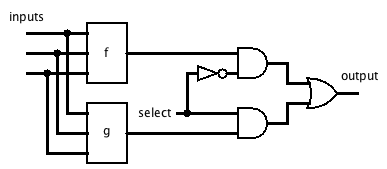
\includegraphics[width=!,height=!,scale=0.75]{graphics/ForG.png}
\end{center}
When \textit{select} is 0, the output is computed by $f$; when it is 1, the output is computed by $g$.

The idea of selecting from two signals may be generalized to using a $k$-bit input to select from one of up to $2^k$ signals; the result is known as a \nw{multiplexer} (often abbreviated MUX). For example, with two select lines, $s_1s_0$, you can choose one of four inputs: $a_{00}$, $a_{01}$, $a_{10}$, or $a_{11}$. Each input is enabled by an appropriate combination of the select lines and their complements, then all four possibilities (of which at most one may be true) are combined with \textsc{or}. Here is the circuit and its common symbol:
\begin{center}
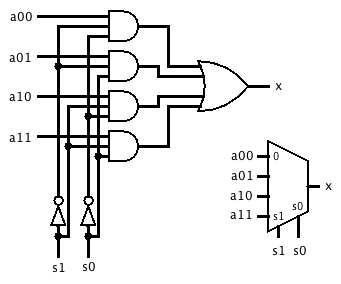
\includegraphics[width=!,height=!,scale=0.75]{graphics/MUX.png}
\end{center}

Note the similarity of the multiplexer circuit to the layers of the sum-of-products circuit from Section~\ref{sec:circsimp}. If we view the input lines $a_{ij}$ as the enabling inputs, then a multiplexer gives a direct way of implementing a truth table: hard-wire the input lines to 0 or 1 according to the corresponding entries in the truth table, then use the select lines to choose the desired row to send to the output. For example, if $a_{01}$ and $a_{10}$ are both tied to 1, while $a_{00}$ and $a_{11}$ are 0, then the output of the multiplexer will be the exclusive-\textsc{or} of $s_1$ and $s_0$.

The opposite of a multiplexer is a \nw{demultiplexer} (DEMUX). It takes one input signal plus $k$ select lines, and delivers the input signal to one of $2^k$ output lines. A special case is known as a \nw{($k$-bit) decoder}: if the input signal is fixed at 1, then the decoder will send a 1 to exactly one of its output lines. Alternately, a demultiplexer can be viewed as a decoder with an ``enable'' input, where the selected output line will be 1 only if the enabling input signal is 1. Here is the common symbol for a four-line demultiplexer:
\begin{center}
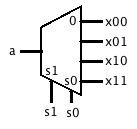
\includegraphics[width=!,height=!,scale=0.75]{graphics/DEMUX.png}
\end{center}
The implementation of this circuit is left as an exercise.

\begin{exercises}
\problem\label{ex:cascade}Compute the total gate delays for a half adder, a full adder, and a four-bit cascaded adder as described in this section. The total delay is the maximum number of gate delays between any input signal changing and all output signals stabilizing to reflect the changed input.

\problem Draw the circuit diagram for an implementation of a four-line demultiplexer.

\problem A \nw{parity bit generator} is a circuit that takes some number of lines of input and produces one output which is 0 if an even number of the inputs are 1, and 1 if an odd number of the inputs are 1. If the input bits are transmitted along with the generated parity bit, then a recipient can check whether any single bit was mis-transmitted by ensuring that the total number of 1 bits received is even. A two-input parity bit generator is just the exclusive-\textsc{or} circuit, whose common symbol is:
\begin{center}
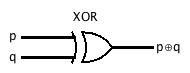
\includegraphics[width=!,height=!,scale=0.75]{graphics/XOR.png}
\end{center}
Give an implementation of a two-input parity bit generator using only \textsc{nand} gates, and then show how to use \textsc{xor} gates to build an eight-input parity bit generator.

\problem The opposite of a decoder is an \nw{encoder}: given $2^k$ input lines, the output will be a $k$-bit binary number representing which input is 1. In case more than one input line is 1, the output will give the highest such line number; this is known as a ``priority encoder.'' For example, when $k=3$, if lines $a_1$, $a_4$, and $a_5$ are all 1, while the rest are 0, then the output will be 101 (5 in binary). If no input line is 1, then the output will be 000. There is one additional output line, $g$ (the ``group'' signal) that will only be 1 if at least one of the inputs is 1; this allows us to tell the difference between no input and only line $a_0$ being 1.

Give a truth table for a four-input ($k=2$) priority encoder, then draw a circuit diagram that implements it.

\end{exercises}

\subsection{Divide-and-Conquer Design}
See Sections~13.5--7 of Aho \& Ullman.

\begin{exercises}
\problem Show how to construct a $2k$-input parity bit generator given a block that implements a $k$-input parity bit generator.

\problem Show how to construct a $2k$-input priority encoder given a block that implements a $k$-input priority encoder.

\end{exercises}



\section{Predicates and Quantifiers}\label{S-logic-4}

In propositional logic,\index{propositional logic} we can let $p$ stand for ``Roses are red'' and
$q$ stand for ``Violets are blue.''  Then $p\AND q$ will stand for
``Roses are red and violets are blue.''  But we lose a lot in the
translation into logic.  Since propositional logic only deals with
truth values, there's nothing we can do with $p$ and $q$ in propositional
logic that has anything to do with roses, violets, or color.
To apply logic to such things, we need \nw[predicate]{predicates}.
The type of logic that uses predicates is called \nw{predicate
logic}, or, when the emphasis is on manipulating and reasoning
with predicates, \nw{predicate calculus}.

A predicate is a kind of incomplete proposition, which becomes
a proposition when it is applied to some entity (or, as we'll see later,
to several entities).  In the proposition ``the rose is red,'' the
predicate is \emph{is red}.  By itself, ``is red'' is not a proposition.
Think of it as having an empty slot, that needs to be filled in
to make a proposition: ``---~is red.''  In the proposition
``the rose is red,'' the slot is filled by the entity ``the rose,''
but it could just as well be filled by other entities:
``the barn is red''; ``the wine is red''; ``the banana is red.''
Each of these propositions uses the same predicate, but they are
different propositions and they can have different truth values.

If $P$ is a predicate and $a$ is an entity, then $P(a)$ stands for
the proposition that is formed when $P$ is applied to $a$.  If $P$
represents ``is red'' and $a$ stands for ``the rose,'' then
$P(a)$ is ``the rose is red.''  If $M$ is the predicate
``is mortal'' and $s$ is ``Socrates,'' then $M(s)$ is the proposition
``Socrates is mortal.'' 

Now, you might be asking, just what is an \emph{entity}\index{entity} anyway?
I am using the term here to mean some specific, identifiable thing
to which a predicate can be applied.  Generally, it doesn't make
sense to apply a given predicate to every possible entity, but only
to entities in a certain category.  For example, it probably doesn't
make sense to apply the predicate ``is mortal'' to your living room
sofa.  This predicate only applies to entities in the category of
living things, since there is no way something can be mortal unless it
is alive.  This category is called the domain of discourse for
the predicate.\footnote{In the language
of set theory, which will be introduced in the next chapter,
we would say that a domain of discourse is a set, $U$, and
a predicate is a function from $U$ to the set of truth values.
The definition should be clear enough without the formal language
of set theory, and in fact you should think of this definition---and
many others---as motivation for that language.}

We are now ready for a formal definition of one-place
predicates.  A one-place
predicate, like all the examples we have seen so far, has a single
slot which can be filled in with one entity:


\begin{definition}
A \nw{one-place predicate}\index{predicate} associates a proposition with each entity in some
collection of entities.  This collection is called the \nw{domain
of discourse} for the predicate.  If $P$ is a predicate and $a$ is
an entity in the domain of discourse for $P$, then $P(a)$ denotes
the proposition that is associated with $a$ by~$P$.  We say that $P(a)$
is the result of \nw[none]{applying} $P$ to~$a$.
\end{definition}

We can obviously extend this to predicates that can be applied to
two or more entities.  In the proposition ``John loves Mary,''
\emph{loves} is a two-place predicate.  Besides John and Mary,
it could be applied to other pairs of entities:  ``John loves Jane,''
``Bill loves Mary,'' ``John loves Bill,''  ``John loves John.''
If $Q$ is a two-place
predicate, then $Q(a,b)$ denotes the proposition that is obtained
when $Q$ is applied to the entities $a$ and~$b$.  Note that each of
the ``slots'' in a two-place predicate can have its own domain of
discourse.  For example, if $Q$ represents the predicate ``owns,''
then $Q(a,b)$ will only make sense when $a$ is a person and $b$ is an
inanimate object.  An example of a three-place predicate is
``$a$~gave $b$ to~$c$,'' and a four-place predicate would be
``$a$~bought $b$ from $c$ for $d$ dollars.''  But keep in mind that
not every predicate has to correspond to an English sentence.

When predicates are applied to entities, the results are propositions,
and all the operators of propositional logic can be applied to these
propositions just as they can to any propositions.  Let $R$ be the
predicate ``is red,'' and let $L$ be the two-place predicate ``loves.''
If $a$, $b$, $j$, $m$, and $b$ are entities belonging to the 
appropriate categories, then we can form compound propositions such
as:
\[
\begin{array}{l@{\qquad}l}
   R(a)\AND R(b)         &\text{$a$ is red and $b$ is red}\\
   \NOT R(a)             &\text{$a$ is not red}\\
   L(j,m)\AND\NOT L(m,j) &\text{$j$ loves $m$, and $m$ does not love $j$}\\
   L(j,m)\IMP L(b,m)     &\text{if $j$ loves $m$ then $b$ loves $m$}\\
   R(a)\IFF L(j,j)       &\text{$a$ is red if and only if $j$ loves $j$}\\
\end{array}
\]


\medbreak
Let's go back to the proposition with which we started this section:
``Roses are red.''  This sentence is more difficult to handle than
it might appear.  We still can't express it properly in logic.
The problem is that this proposition is not saying something about
some particular entity.  It really says that \emph{all} roses are red 
(which happens to be a false statement, but that's what it means).
Predicates can only be applied to individual entities.

Many other sentences raise similar difficulties:
``All persons are mortal.''  ``Some roses are red, but no roses are black.''
``All math courses are interesting.''  ``Every prime number greater than two
is odd.''  Words like \emph{all}, \emph{no}, \emph{some}, and \emph{every}
are called \nw{quantifiers}.\index{quantifier!in English}  We need to be able to express similar concepts
in logic.

Suppose that $P$ is a predicate, and we want to express the proposition that
$P$ is true when applied to any entity in the domain of discourse.
That is, we want to say ``for any entity $x$ in the domain of discourse,
$P(x)$ is true.''  In predicate logic, we write this in symbols as
$\forall x(P(x))$.  The $\forall$ symbol, which looks like an
upside-down~A, is usually read ``for all,'' so that $\forall x(P(x))$
is read as ``for all $x$, $P(x)$.''  (It is understood that this means
for all $x$ in the domain of discourse for~$P$.)  For example,
if $R$ is the predicate ``is red'' and the domain of discourse consists
of all roses, then $\forall x(R(x))$ expresses the proposition
``All roses are red.''  Note that the same proposition could be
expressed in English as ``Every rose is red'' or ``Any rose is red.''
 
Now, suppose we want to say that a predicate, $P$, is true for \emph{some}
entity in its domain of discourse.  This is expressed in predicate
logic as $\exists x(P(x))$.  The $\exists$ symbol, which looks like a
backwards~E, is usually read ``there exists,'' but a more exact reading
would be ``there is at least one.'' Thus, $\exists x(P(x))$ is read
as ``There exists an $x$ such that $P(x)$,'' and it means ``there is
at least one $x$ in the domain of discourse for $P$ for which $P(x)$
is true.''  If, once again, $R$ stands for ``is red'' and the domain
of discourse is ``roses,'' then $\exists x(R(x))$ could be expressed
in English as ``There is a red rose'' or ``At least one rose is red''
or ``Some rose is red.''  It might also be expressed as ``Some roses
are red,'' but the plural is a bit misleading since $\exists x(R(x))$
is true even if there is only one red rose.
We can now give the formal definitions:

\begin{definition}
Suppose that $P$ is a one-place predicate.  Then $\forall x(P(x))$ is
a proposition, which is true if and only if $P(a)$ is true for every
entity $a$ in the domain of discourse for~$P$.  And $\exists x(P(x))$
is a proposition which is true if and only if there is at least one
entity, $a$, in the domain of discourse for $P$ for which $P(a)$ is
true.  The $\forall$ symbol is called the \nw{universal quantifier},
and $\exists$ is called the \nw{existential quantifier}.
\end{definition}

The $x$ in $\forall x(P(x))$ and $\exists x(P(x))$ is a variable.\index{variable}
(More precisely, it is an \emph{entity} variable, since its value
can only be an entity.)\index{entity!variable}
Note that a plain $P(x)$---without the $\forall x$ or $\exists x$---is
not a proposition.  $P(x)$~is neither true nor false because $x$
is not some particular entity, but just a placeholder in a slot that
can be filled in with an entity.  $P(x)$~would stand for
something like the statement ``$x$~is red,'' which is not really a
statement in English at all.  But it becomes a statement when
the $x$ is replaced by some particular entity, such as ``the rose.''
Similarly, $P(x)$ becomes a proposition if some entity $a$ is substituted
for the~$x$, giving $P(a)$.\footnote{There is certainly room for confusion
about names here.  In this discussion, $x$ is a variable and $a$ is 
an entity.  But that's only because I said so.  Any letter could be used
in either role, and you have to pay attention to the context to
figure out what is going on.  Usually, $x$, $y$, and $z$ will be variables.}

An \nw{open statement} is an expression that contains one or more entity
variables, which becomes a proposition when entities are substituted
for the variables.  (An open statement has open ``slots'' that need to
be filled in.)  $P(x)$ and ``$x$ is red'' are examples of open 
statements that contain one variable.  If $L$ is a two-place predicate
and $x$ and $y$ are variables, then $L(x,y)$ is an open statement
containing two variables.  An example in English would be
``$x$~loves~$y$.''  The variables in an open statement are called 
\nw[free variable]{free variables}.  An open statement that contains $x$ as a free
variable can be quantified with $\forall x$ or $\exists x$.
The variable $x$ is then said to be \nw[bound variable]{bound}.  For example,
$x$ is free in $P(x)$ and is bound in $\forall x(P(x))$ and
$\exists x(P(x))$.  The free variable $y$ in $L(x,y)$ becomes
bound in $\forall y(L(x,y))$ and in $\exists y(L(x,y))$.

Note that $\forall y(L(x,y))$ is still an open statement, since
it contains $x$ as a free variable.\index{quantifier!on a two-place predicate}
Therefore, it is possible to
apply the quantifier $\forall x$ or $\exists x$ to $\forall y(L(x,y))$,
giving $\forall x\big(\forall y(L(x,y))\big)$ and
$\exists x\big(\forall y(L(x,y))\big)$.  Since all the variables are
bound in these expressions, they are propositions.  If $L(x,y)$ represents
``$x$~loves~$y$,'' then $\forall y(L(x,y))$ is something like ``$x$~loves
everyone,''  and $\exists x\big(\forall y(L(x,y))\big)$ is the
proposition, ``There is someone who loves everyone.''  Of course, we
could also have started with $\exists x(L(x,y))$: ``There is someone
who loves~$y$.''  Applying $\forall y$ to this gives 
$\forall y\big(\exists x(L(x,y))\big)$,
which means ``For every person, there is someone who loves that person.''
Note in particular that $\exists x\big(\forall y(L(x,y))\big)$ and
$\forall y\big(\exists x(L(x,y))\big)$ do \emph{not} mean the same thing.
Altogether, there are eight different propositions that can
be obtained from $L(x,y)$ by applying quantifiers, with six distinct
meanings among them.

(From now on, I will leave out parentheses when there is no ambiguity.
For example, I will write $\forall x\, P(x)$ instead of $\forall x(P(x))$
and $\exists x\,\exists y\,L(x,y)$ instead of
$\exists x\big(\exists y(L(x,y))\big)$.  Furthermore, I will
sometimes give predicates and entities names that are complete words
instead of just letters, as in  $Red(x)$ and $Loves(john,mary)$.
This might help to make examples more readable.)

\medbreak

In predicate logic, the operators and laws of Boolean algebra\index{Boolean algebra!in predicate logic} still
apply.  For example, if $P$ and $Q$ are one-place predicates and
$a$ is an entity in the domain of discourse, then $P(a)\IMP Q(a)$
is a proposition, and it is logically equivalent to $\NOT P(a)\OR Q(a)$.
Furthermore, if $x$ is a variable, then $P(x)\IMP Q(x)$ is an open
statement, and $\forall x(P(x)\IMP Q(x))$ is a proposition.
So are $P(a)\AND(\exists x\,Q(x))$ and $(\forall x\,P(x))\IMP(\exists xP(x))$.
Obviously, predicate logic can be very expressive.  Unfortunately,
the translation between predicate logic and English sentences is not
always obvious.

Let's look one more time at the proposition ``Roses are red.''
If the domain of discourse consists of roses, this translates into
predicate logic as $\forall x\, Red(x)$.  However, the sentence makes
more sense if the domain of discourse is larger---for example if it
consists of all flowers.  Then ``Roses are red'' has to be read as
``All flowers which are roses are red,'' or ``For any flower,
if that flower is a rose, then it is red.'' The last form translates
directly into logic as $\forall x\big(Rose(x)\IMP Red(x)\big)$.
Suppose we want to say that all red roses are pretty.  The phrase
``red rose'' is saying both that the flower is a rose and that it is
red, and it must be translated as a conjunction, $Rose(x)\AND Red(x)$.
So, ``All red roses are pretty'' can be rendered as
$\forall x\big((Rose(x)\AND Red(x))\IMP Pretty(x)\big)$.

Here are a few more examples of translations from predicate logic
to English.  Let $H(x)$ represent ``$x$~is happy,'' let
$C(y)$~represent ``$y$~is a computer,'' and let $O(x,y)$~represent
``$x$~owns~$y$.''  (The domain of discourse for $x$ consists of 
people, and the domain for $y$ consists of inanimate objects.)
Then we have the following translations:

\begin{itemize}
\setlength{\itemsep}{0pt plus 1 pt}
\setlength{\parsep}{0pt plus 1 pt}
\item Jack owns a computer: $\exists x\big(O(jack,x)\AND C(x)\big)$.
(That is, there is at least one thing such that Jack owns that thing and that thing
is a computer.)
\item Everything Jack owns is a computer: $\forall x\big(O(jack,x)\IMP C(x)\big)$.
\item If Jack owns a computer, then he's happy:\\*
\hspace*{0.5in}$\big(\exists y(O(jack,y)\AND C(y))\big)\IMP H(jack)$.
\item Everyone who owns a computer is happy:\\*
\hspace*{0.5in} $\forall x\big(\,\big(\exists y(O(x,y)\AND C(y)\big)\IMP H(x)\big)\,\big)$.
\item Everyone owns a computer: $\forall x\,\exists y\big(C(y)\AND O(x,y)\big)$.
(Note that this allows each person to own a different computer.
The proposition $\exists y\,\forall x\big(C(y)\AND O(x,y)\big)$
would mean that there is a single computer which is owned by
everyone.)
\item Everyone is happy: $\forall xH(x)$.
\item Everyone is unhappy: $\forall x(\NOT H(x))$.
\item Someone is unhappy: $\exists x(\NOT H(x))$.
\item At least two people are happy:
 $\exists x \exists y\big(H(x) \AND H(y) \AND (x\ne y)\big)$.  (The stipulation
 that $x\ne y$ is necessary because two different variables can refer to
 the same entity.  The proposition $\exists x\exists y(H(x)\AND H(y))$ is
 true even if there is only one happy person.)
\item There is exactly one happy person:\\*
 \hspace*{0.5 in}$\big(\exists x H(x)\big)) \AND \big(\forall y \forall z((H(y)\AND H(z))\IMP (y=z))\big)$.
 (The first part of this conjunction says that there is at least one happy person.
 The second part says that if $y$ and $z$ are both happy people, then they are actually
 the same person. That is, it's not possible to find two \emph{different} people who
 are happy.)
\end{itemize}

\medskip

To calculate in predicate logic, we need a notion of logical equivalence.
Clearly, there are pairs of propositions in predicate logic that mean the same
thing.  Consider the propositions $\NOT(\forall x H(x))$ and $\exists x(\NOT H(x))$, where
$H(x)$ represents ``$x$~is happy.'' The first of these propositions means
``Not everyone is happy,'' and the second means ``Someone is not happy.''
These statements have the same truth value:  If not everyone is happy, then someone is
unhappy and vice versa.  But logical equivalence is much stronger than just
having the same truth value.  In propositional logic, logical equivalence
is defined in terms of propositional variables:  two compound propositions
are logically equivalent if they have the same truth values for all possible
truth values of the propositional variables they contain.  In predicate logic, two
formulas are logically equivalent\index{logical equivalence!in predicate logic}
if they have the same truth value for all
possible predicates.

Consider $\NOT(\forall x P(x))$ and $\exists x(\NOT P(x))$.\index{negation!of quantified statements}
These formulas make
sense for any predicate $P$, and for any predicate $P$ they have the same truth
value.  Unfortunately, we can't---as we did in propositional logic---just check
this fact with a truth table: there are no subpropositions, connected by
$\AND$, $\OR$, etc, out of which to build a table.  So, let's reason it out:
To say $\NOT(\forall x P(x))$ is true is just to say that it is not the case that
$P(x)$ is true for all possible entities $x$.  So, there must be some entity $a$
for which $P(a)$ is false.  Since $P(a)$ is false, $\NOT P(a)$ is true.
But saying that there is an $a$ for which $\NOT P(a)$ is true is just saying
that $\exists x(\NOT P(x))$ is true.  So, the truth of $\NOT(\forall x P(x))$
implies the truth of $\exists x (\NOT P(x))$.  On the other hand, if 
$\NOT(\forall x P(x))$ is false, then $\forall x P(x)$ is true.  Since $P(x)$
is true for every~$x$, $\NOT P(x)$ is false for every~$x$; that is, there is no
entity $a$ for which the statement $\NOT P(a)$ is true.
But this just means that the statement $\exists x(\NOT P(x))$
is false.  In any case, then, the truth values of $\NOT(\forall x P(x))$ and
$\exists x(\NOT P(x))$ are the same.  Since this is true for any predicate $P$,
we will say that these two formulas are logically equivalent and write
$\NOT(\forall x P(x)) \equiv \exists x(\NOT P(x))$.

\fig
  {F-predlogic}
  {Four important rules of predicate logic.  $P$ can be any one-place predicate,
   and $Q$ can be any two-place predicate.  The first two rules are called
   DeMorgan's Laws for predicate logic.}
  {\begin{tabular}{|c|}
     \hline
     \strut$\NOT\,(\forall x P(x)) \equiv \exists x(\NOT P(x))$\\
     \hline
     \strut$\NOT\,(\exists x P(x)) \equiv \forall x(\NOT P(x))$\\
     \hline
     \strut$\forall x \forall y Q(x,y) \equiv \forall y \forall x Q(x,y)$\\
     \hline
     \strut$\exists x \exists y Q(x,y) \equiv \exists y \exists x Q(x,y)$\\
     \hline
  \end{tabular}
 }

A similar argument would show that $\NOT(\exists x P(x)) \equiv \forall x(\NOT P(x))$.
These two equivalences, which explicate the relation between negation and quantification,
are known as DeMorgan's Laws\index{DeMorgan's Laws} for predicate logic.  (They are closely related to
DeMorgan's Laws for propositional logic; see the exercises.)  These
laws can be used to help simplify expressions.  For example, 
\begin{align*}
  \NOT\,\forall y (R(y)\OR Q(y)) &\equiv \exists y(\NOT(R(y)\OR Q(y)))\\
       &\equiv \exists y((\NOT R(y))\AND(\NOT Q(y))\\
\end{align*}
It might not be clear exactly why this qualifies as a ``simplification,''
but it's generally considered simpler to have the negation operator applied
to basic propositions such as $R(y)$, rather than to quantified expressions
such as \hbox{$\forall y (R(y)\OR Q(y))$}.
For a more complicated example:
\begin{align*}
  \NOT\,\exists x\big(P(x)&\AND (\forall y (Q(y)\IMP Q(x)))\big)\\
            &\equiv\forall x\big(\NOT\big(P(x)\AND (\forall y (Q(y)\IMP Q(x)))\big)\\
            &\equiv\forall x\big((\NOT P(x))\OR (\NOT \forall y (Q(y)\IMP Q(x)))\big)\\
            &\equiv\forall x\big((\NOT P(x))\OR (\exists y(\NOT (Q(y)\IMP Q(x))))\big)\\
            &\equiv\forall x\big((\NOT P(x))\OR (\exists y(\NOT (\NOT Q(y)\OR Q(x))))\big)\\
            &\equiv\forall x\big((\NOT P(x))\OR (\exists y(\NOT\NOT Q(y)\AND \NOT Q(x)))\big)\\
            &\equiv\forall x\big((\NOT P(x))\OR (\exists y(Q(y)\AND \NOT Q(x)))\big)\\
\end{align*}
DeMorgan's Laws are listed in Figure~\ref{F-predlogic} along with two
other laws of predicate logic.  The other laws allow you to interchange
the order of the variables when two quantifiers of the same type
(both $\exists$ or $\forall$) occur together. 

To define logical equivalence in predicate logic more formally,
we need to talk about formulas that contain predicate variables,\index{variable}
that is, variables that act as place-holders for arbitrary predicates
in the same way that propositional variables are place-holders for
propositions and entity variables are place-holders for
entities.  With this in mind, we can define logical equivalence
and the closely related concept of tautology for predicate logic.

\begin{definition}
Let $\mathscr{P}$ be a formula of predicate logic which contains one or more
predicate variables.  $\mathscr{P}$~is said to be a \nw{tautology}
if it is true whenever all the predicate variables that it contains are replaced
by actual predicates.  Two formulas $\mathscr{P}$ and $\mathscr{Q}$ are
said to be \nw[logical equivalence!in predicate logic]{logically equivalent} if $\mathscr{P}\IFF\mathscr{Q}$ is
a tautology, that is if $\mathscr{P}$ and $\mathscr{Q}$ always have the same
truth value when the predicate variables they contain are replaced by actual
predicates.  The notation $\mathscr{P}\equiv\mathscr{Q}$ asserts that
$\mathscr{P}$ is logically equivalent to $\mathscr{Q}$.
\end{definition}




\begin{exercises}

\problem Simplify each of the following propositions.  In your answer, the
$\NOT$ operator should be applied only to individual predicates.
\pparts{
   \NOT\,\forall x (\NOT P(x)) & \NOT\,\exists x(P(x)\AND Q(x))\cr
   \NOT \,\forall z(P(z)\IMP Q(z))&
      \NOT\big((\forall x P(x))\AND \forall y(Q(y))\big) \cr
   \NOT\, \forall x \exists y P(x,y)&
      \NOT\,\exists x (R(x)\AND \forall y S(x,y))\cr
    \NOT\,\exists y(P(y)\IFF Q(y))&
       \NOT \big(\forall x (P(x)\IMP (\exists y Q(x,y)))\big) \cr
}

\problem Give a careful argument to show that the second of DeMorgan's laws for
predicate calculus,
$\NOT(\forall x P(x)) \equiv \exists x(\NOT P(x))$, is valid.

\problem Find the negation of each of the following propositions.
Simplify the result; in your answer, the
$\NOT$ operator should be applied only to individual predicates.
\ppart $\NOT$$\exists n (\forall s C(s,n))$
\ppart $\NOT$$\exists n (\forall s (L(s,n) \IMP P(s)))$
\ppart $\NOT$$\exists n (\forall s (L(s,n) \IMP (\exists x \exists y \exists z Q(x,y,z))))$.
\ppart $\NOT$$\exists n (\forall s (L(s,n) \IMP (\exists x \exists y \exists z (s=xyz \AND 
R(x,y) \AND T(y) \AND U(x,y,z))))$.

\problem Suppose that the domain of discourse for a predicate $P$
contains only two entities.  Show that $\forall x P(x)$ is equivalent to
a conjunction of two simple propositions, and $\exists x P(x)$ is equivalent
to a disjunction.  Show that in this case, DeMorgan's Laws for propositional
logic and DeMorgan's Laws for predicate logic actually say exactly the same
thing.  Extend the results to a domain of discourse that contains exactly
three entities.

\problem Let $H(x)$ stand for ``$x$ is happy,'' where the domain of discourse
consists of people.  Express the proposition ``There are exactly three happy
people'' in predicate logic.

\problem Let $T(x,y)$ stand for ``$x$~has taken~$y$,'' where the
domain of discourse for $x$ consists of students and the domain
of discourse for $y$ consists of math courses (at your school).
Translate each of the following propositions into an unambiguous English sentence:
\pparts{ \forall x\,\forall y \,T(x,y) & \forall x \,\exists y \,T(x,y) & \forall y \,\exists x \,T(x,y)\cr
         \exists x\,\exists y \,T(x,y) & \exists x \,\forall y \,T(x,y) & \exists y \,\forall x \,T(x,y)\cr
}

\problem Let $F(x,t)$ stand for ``You can fool person $x$ at time~$t$.''
Translate the following sentence into predicate logic:
``You can fool some of the people all of the time, and you can fool
all of the people some of the time, but you can't fool all of the
people all of the time.''

\problem Translate each of the following sentences into a proposition 
using predicate logic.  Make up any predicates you need.  State what
each predicate means and what its domain of discourse is.
\ppart All crows are black.
\ppart Any white bird is not a crow.
\ppart Not all politicians are honest.
\ppart All green elephants have purple feet.
\ppart There is no one who does not like pizza.
\ppart Anyone who passes the final exam will pass the course.
\ppart If $x$ is any positive number, then there is a number $y$ such that
$y^2=x$.

\problem The sentence ``Someone has the answer to every question'' is
ambiguous.  Give two translations of this sentence into predicate logic,
and explain the difference in meaning.

\problem The sentence ``Jane is looking for a dog'' is ambiguous.
One meaning is that there is some particular dog---maybe the one she lost---that
Jane is looking for.  The other meaning is that Jane is looking for any old
dog---maybe because she wants to buy one.  Express the first meaning in
predicate logic.  Explain why the second meaning is \emph{not}
expressed by $\forall x(Dog(x)\IMP LooksFor(jane,x))$.  In fact, the
second meaning cannot be expressed in predicate logic.  Philosophers
of language spend a lot of time thinking about things like this.
They are especially fond of the sentence ``Jane is looking for a unicorn,''
which is not ambiguous when applied to the real world.  Why is that?



\end{exercises}



\section{Deduction}\label{S-logic-5}


\newcommand{\argument}[2]{
  \begin{tabular}[t]{@{\ }l@{\ }}
   #1\\
   \hline
   $\therefore$\ \ #2\\
  \end{tabular}
}


Logic can be applied to draw conclusions from a set of premises.
A premise\index{premise} is just a proposition that is known to be true or that
has been accepted to be true for the sake of argument, and a conclusion\index{conclusion}
is a proposition that can be deduced\index{deduction} logically from the premises.
The idea is that if you believe that the premises are true,
then logic forces you to accept that the conclusion is true.
An ``argument''\index{argument} is a claim that a certain conclusion follows from
a given set of premises.  Here is an argument laid out in
a traditional format:
\begin{center}
\argument{If today is Tuesday, then this is Belgium\\Today is Tuesday}{This is Belgium}
\end{center}
The premises of the argument are shown above the line, and the conclusion
below.  The symbol $\therefore$ is read ``therefore.''  The claim is that
the conclusion, ``This is Belgium,'' can be deduced logically from the two
premises, ``If today is Tuesday, then this is Belgium'' and ``Today is Tuesday.''
In fact, this claim is true.  Logic forces you to accept this argument.
Why is that?

Let $p$ stand for the proposition ``Today is Tuesday,'' and let $q$ stand for the
proposition ``This is Belgium.''  Then the above argument has the form
\begin{center}
\argument{$p\IMP q$\\$p$}{$q$}
\end{center}
Now, for \emph{any} propositions $p$ and $q$---not just the ones in this particular
argument---if $p\IMP q$ is true and $p$ is true, then $q$ must also be true.
This is easy to check in a truth table:
\begin{center}
  \begin{tabular}{|c|c|c|}
     \hline
     \strut $p$&    $q$&    $p\IMP q$\\
     \hline
     false&  false&  true\\
     false&  true&   true\\
     true&   false&  false\\
     true&   true&   true\\
     \hline
  \end{tabular}
\end{center}
The only case where both $p\IMP q$ and $p$ are true is on
the last line of the table, and in this case, $q$ is also true.
If you believe
$p\IMP q$ and $p$, you have no logical choice but to believe $q$.
This applies no matter what $p$ and $q$ represent.  For example,
if you believe ``If Jill is breathing, then Jill pays taxes,'' 
and you believe that ``Jill is breathing,'' logic forces you to believe that
``Jill pays taxes.''  Note that we can't say for sure that the
conclusion is true, only that \emph{if} the premises are true,
\emph{then} the conclusion must be true.

This fact can be rephrased by saying that $\big((p\IMP q)\AND p\big)\IMP q$
is a tautology.  More generally, for any compound propositions $\mathscr{P}$
and $\mathscr{Q}$, saying ``$\mathscr{P}\IMP \mathscr{Q}$ is
a tautology'' is the same as saying that ``in all cases where $\mathscr{P}$
is true, $\mathscr{Q}$ is also true''.\footnote{Here, ``in all cases'' means
for all combinations of truth values of the propositional variables
in $\mathscr{P}$ and $\mathscr{Q}$.  Saying $\mathscr{P}\IMP \mathscr{Q}$ is
a tautology means it is true in all cases.  But by definition of 
$\IMP$, it is automatically true in cases where $\mathscr{P}$ is
false.  In cases where $\mathscr{P}$ is true, $\mathscr{P}\IMP \mathscr{Q}$
will be true if and only if $\mathscr{Q}$ is true.}
We will use the notation $\mathscr{P}\LOGIMP\mathscr{Q}$ to
mean that $\mathscr{P}\IMP \mathscr{Q}$ is a tautology.
Think of $\mathscr{P}$ as being the premise of an argument or
the conjunction of several premises.  To say $\mathscr{P}\LOGIMP\mathscr{Q}$
is to say that $\mathscr{Q}$ follows logically from~$\mathscr{P}$.
We will use the same notation in both propositional logic and
predicate logic.  (Note that the relation of $\LOGIMP$ to $\IMP$ is
the same as the relation of $\equiv$ to $\IFF$.)


\begin{definition}
Let $\mathscr{P}$ and $\mathscr{Q}$ be any formulas in either
propositional logic or predicate logic.  The notation
$\mathscr{P}\LOGIMP\mathscr{Q}$ is used to mean that
$\mathscr{P}\IMP\mathscr{Q}$ is a tautology.  That is,
in all cases where $\mathscr{P}$ is true, $\mathscr{Q}$ is
also true.  We then say that $\mathscr{Q}$ can be
\nw[deduction]{logically deduced} from $\mathscr{P}$ or that
$\mathscr{P}$ \nw{logically implies} $\mathscr{Q}$.
\end{definition}

An argument in which the conclusion follows logically from the
premises is said to be a \nw{valid argument}.  To test whether
an argument is valid, you have to replace the particular propositions
or predicates that it contains with variables, and then test
whether the conjunction of the premises logically implies the
conclusion.  We have seen that any argument of the form
\begin{center}
\argument{$p\IMP q$\\$p$}{$q$}
\end{center}
is valid, since $\big((p\IMP q)\AND p\big)\IMP q$ is a tautology.
This rule of deduction is called \nw{modus ponens}.  It plays a central
role in logic.  Another, closely related rule is \nw{modus tollens},
which applies to arguments of the form
\begin{center}
\argument{$p\IMP q$\\$\NOT q$}{$\NOT p$}
\end{center}
To verify that this is a valid argument, just check that
$\big((p\IMP q)\AND \NOT q\big)\LOGIMP \NOT p$, that is, that
$\big((p\IMP q)\AND \NOT q\big)\IMP \NOT p$ is a tautology.
As an example, the following argument has the form of \textit{modus tollens}
and is therefore a valid argument:
\begin{center}
\argument{If Keanu Reeves is a good actor, then I'm the king of France\\
I am not the king of France}{Keanu Reeves in not a good actor}
\end{center}
You should note carefully that the validity of this argument has nothing
to do with whether or not Keanu Reeves\index{Reeves, Keanu} can act well.  The argument forces
you to accept the conclusion \emph{only if} you accept the premises.
You can logically believe that the conclusion is false, as long as
you believe that at least one of the premises is false.

Another named rule of deduction is the \nw[syllogism]{Law of Syllogism}, which has the form
\begin{center}
\argument{$p\IMP q$\\$q\IMP r$}{$p\IMP r$}
\end{center}
For example:
\begin{center}
\argument{If you study hard, you do well in school\\
If you do well in school, you get a good job}{If you study hard,
you get a good job}
\end{center}

There are many other rules.  Here are a few that might prove useful.
Some of them might look trivial, but don't underestimate the power
of a simple rule when it is combined with other rules.
\begin{center}
\mbox{
\argument{$p\OR q$\\$\NOT p$}{$q$}\qquad
\argument{$p$\\$q$}{$p\AND q$}\qquad
\argument{$p\AND q$}{$p$}\qquad
\argument{$p$}{$p\OR q$}
}
\end{center}


Logical deduction is related to logical equivalence.\index{logical equivalence!and logical deduction}
We defined $\mathscr{P}$ and $\mathscr{Q}$ to be
logically equivalent if $\mathscr{P}\IFF\mathscr{Q}$ is
a tautology.  Since $\mathscr{P}\IFF\mathscr{Q}$ is equivalent
to $(\mathscr{P}\IMP\mathscr{Q})\AND(\mathscr{Q}\IMP\mathscr{P})$,
we see that  $\mathscr{P}\equiv \mathscr{Q}$ if and only if both
$\mathscr{Q}\LOGIMP\mathscr{P}$ and $\mathscr{P}\LOGIMP\mathscr{Q}$.
Thus, we can show that two statements are logically equivalent if
we can show that each of them can be logically deduced from the
other.  Also, we get a lot of rules about logical deduction for 
free---two rules of deduction for each logical equivalence we know.  For
example, since $\NOT(p\AND q)\equiv (\NOT p\OR \NOT q)$,
we get that $\NOT(p\AND q)\LOGIMP (\NOT p\OR \NOT q)$.
For example, if we know  ``It is not both sunny and warm,'' 
then we can logically deduce ``Either it's not sunny or it's not warm.''
(And vice versa.)


\medskip


In general, arguments are more complicated that those we've considered
so far.  Here, for example, is an argument that has five premises:
\begin{center}
\argument{
  $(p\AND r)\IMP s$\\
  $q\IMP p$\\
  $t\IMP r$\\
  $q$\\
  $t$
}{$s$}
\end{center}
Is this argument valid?  Of course, you could use a truth table
to check whether the conjunction of the premises logically implies
the conclusion.  But with five propositional variables, the table
would have 32 lines, and the size of the table grows quickly when
more propositional variables are used.  So, in general, truth
tables are not practical.  

Fortunately, there is another way to proceed, based on the fact that
it is possible to chain several logical deductions together.
That is, if $\mathscr{P}\LOGIMP\mathscr{Q}$ and
$\mathscr{Q}\LOGIMP\mathscr{R}$, it follows that
$\mathscr{P}\LOGIMP\mathscr{R}$.  This means we can demonstrate the
validity of an argument by deducing the conclusion from the
premises in a sequence of steps.  These steps can be presented
in the form of a proof:

\begin{definition}
A \nw[proof]{formal proof} that an argument is valid consists of a
sequence of propositions such that the last proposition in the
sequence is the conclusion of the argument, and every proposition
in the sequence is either a premise of the argument or follows
by logical deduction from propositions that precede it in the list.
\end{definition}

The existence of such a proof shows that the conclusion follows
logically from the premises, and therefore that the argument is 
valid.\index{valid argument}  Here is a formal proof that the argument given above is valid.
The propositions in the proof are numbered, and each proposition
has a justification.
\begin{center}
  \begin{tabular}{r@{\ \ }l@{\qquad}l}
     1.&$q\IMP p$&    premise\\
     2.&$q$&          premise\\
     3.&$p$&          from 1 and 2 (\textit{modus ponens})\\
     4.&$t\IMP r$&    premise\\
     5.&$t$&          premise\\
     6.&$r$&          from 4 and 5 (\textit{modus ponens})\\
     7.&$p\AND r$&    from 3 and 6\\
     8.&$(p\AND r)\IMP s$& premise\\
     9.&$s$&          from 7 and 8 (\textit{modus ponens})\\
  \end{tabular}
\end{center}
Once a formal proof has been constructed, it is convincing.  Unfortunately,
it's not necessarily easy to come up with the proof.  Usually, the best
method is a combination of working forward (``Here's what I know, what
can I deduce from that?'') and working backwards (``Here's what I
need to prove, what other things would imply that?'').  For this proof,
I might have thought:  I want to prove $s$.  I know that
$p\AND r$ implies $s$, so if I can prove $p\AND r$, I'm OK.
But to prove $p\AND r$, it'll be enough to prove $p$ and $r$ 
separately\dots.

Of course, not every argument is valid, so the question also
arises, how can we show that an argument is invalid?\index{invalid argument}  Let's
assume that the argument has been put into general form, with
all the specific propositions replaced by propositional variables.
The argument is valid if in all cases where all the premises are
true, the conclusion is also true.  The argument is invalid if
there is even one case where all the premises are true and the
conclusion is false.  We can prove that an argument is invalid
by finding an assignment of truth values to the propositional variables
which makes all the premises true but makes the conclusion false.
For example, consider an argument of the form:
\begin{center}
\argument{$p\IMP q$\\$q\IMP (p\AND r)$\\$r$}{$p$}
\end{center}
In the case where $p$ is false, $q$ is false, and $r$ is true,
the three premises of this argument are all true, but the conclusion
is false.  This shows that the argument is invalid.

To apply all this to arguments stated in English, we have to
introduce propositional variables to represent all the propositions
in the argument.  For example, consider:
\begin{quote}
John will be at the party if Mary is there and Bill is not there.
Mary will be at the party if it's on Friday or Saturday.
If Bill is at the party, Tom will be there.  Tom won't be at
the party if it's on Friday.  The party is on Friday.
Therefore, John will be at the party.
\end{quote}
Let $j$ stand for ``John will be at the party,'' $m$ for
``Mary will be there,'' $b$ for ``Bill will be there,''
$t$ for ``Tom will be there,'' $f$ for ``The party is on Friday,''
and $s$ for ``The party is on Saturday.''  Then this argument has
the form
\begin{center}
\argument{$(m\AND \NOT b)\IMP j$\\
  $(f\OR s)\IMP m$\\
  $b\IMP t$\\
  $f\IMP \NOT t$\\
  $f$}{$j$}
\end{center}
This is a valid argument, as the following proof shows:
\begin{center}
  \begin{tabular}{r@{\ \ }l@{\qquad}l}
     1.&$f\IMP\NOT t$&premise\\
     2.&$f$&premise\\
     3.&$\NOT t$&from 1 and 2 (\textit{modus ponens})\\
     4.&$b\IMP t$&premise\\
     5.&$\NOT b$&from 4 and 3 (\textit{modus tollens})\\
     6.&$f\OR s$&from 2\\
     7.&$(f\OR s)\IMP m$&premise\\
     8.&$m$&from 6 and 7 (\textit{modus ponens})\\
     9.&$m\AND\NOT b$&from 8 and 5\\
     10.&$(m\AND\NOT b)\IMP j$&premise\\
     11.&$j$&from 10 and 9 (\textit{modus ponens})\\
  \end{tabular}
\end{center}

\medskip

So far in this section, we have been working mostly with propositional
logic.  But the definitions of valid argument and logical deduction
apply to predicate logic as well.  One of the most basic rules of
deduction in predicate logic says that $(\forall xP(x))\LOGIMP P(a)$
for any entity $a$ in the domain of discourse of the predicate~$P$.
That is, if a predicate is true of all entities, then it is true of
any given particular entity.  This rule can be combined with 
rules of deduction for propositional logic to give the following
valid arguments
\begin{center}
\mbox{
\argument{$\forall x(P(x)\IMP Q(x))$\\$P(a)$}{$Q(a)$}\qquad\qquad
\argument{$\forall x(P(x)\IMP Q(x))$\\$\NOT Q(a)$}{$\NOT P(a)$}
}
\end{center}
These valid arguments go by the names of \textit{modus ponens}\index{modus ponens} and
\textit{modus tollens}\index{modus tollens} for predicate logic.
Note that from the premise $\forall x(P(x)\IMP Q(x))$ we can deduce
$P(a)\IMP Q(a)$.  From this and from the premise that $P(a)$, we
can deduce $Q(a)$ by \textit{modus ponens}.  So the first argument
above is valid.  The second argument is similar, using 
\textit{modus tollens}.

The most famous logical deduction of them all is an application
of \textit{modus ponens} for predicate logic:
\begin{center}
\argument{All humans are mortal\\Socrates is human}{Socrates is mortal}
\end{center}
This has the form of \textit{modus ponens} with $P(x)$ standing
for ``$x$~is human,'' $Q(x)$ standing for ``$x$~is mortal,'' and
$a$ standing for the noted entity, Socrates.

There is a lot more to say about logical deduction and
proof in predicate logic, and we'll spend the rest of this chapter
on the subject.

\begin{exercises}

\problem Verify the validity of \textit{modus tollens} and the Law of
Syllogism.

\problem Each of the following is a valid rule of deduction.
For each one, give an example of a valid argument in English that
uses that rule.
\begin{center}
\mbox{\qquad
\argument{$p\OR q$\\$\NOT p$}{$q$}\qquad
\argument{$p$\\$q$}{$p\AND q$}\qquad
\argument{$p\AND q$}{$p$}\qquad
\argument{$p$}{$p\OR q$}
}
\end{center}

\problem There are two notorious invalid arguments that look
deceptively like \textit{modus ponens} and \textit{modus tollens}:
\begin{center}
\mbox{\qquad
\argument{$p\IMP q$\\$q$}{$p$}\qquad
\argument{$p\IMP q$\\$\NOT p$}{$\NOT q$}\qquad
}
\end{center}
Show that each of these arguments is invalid.  Give an English
example that uses each of these arguments.

\problem Decide whether each of the following arguments is valid.
If it is valid, give a formal proof.  If it is invalid, show that
it is invalid by finding an appropriate assignment of truth values
to propositional variables.
\smallskip
\tparts{
   \argument{$p\IMP q$\\$q\IMP s$\\$s$}{$p$}&
   \argument{$p\AND q$\\$q\IMP (r\OR s)$\\$\NOT r$}{$s$}&
   \argument{$p\OR q$\\$q\IMP (r\AND s)$\\$\NOT p$}{$s$}\cr\noalign{\smallskip}
   \argument{$(\NOT p)\IMP t$\\$q\IMP s$\\$r\IMP q$\\$\NOT(q\OR t)$}{$p$}&
   \argument{$p$\\$s\IMP r$\\$q\OR r$\\$q\IMP\NOT p$}{$\NOT s$}&
   \argument{$q\IMP t$\\$p\IMP(t\IMP s)$\\$p$}{$q\IMP s$}
}


\problem For each of the following English arguments, express the
argument in terms of propositional logic and determine whether the
argument is valid or invalid.
\ppart If it is Sunday, it rains or snows.  Today, it is Sunday
and it's not raining.  Therefore, it must be snowing.
\ppart If there are anchovies on the pizza, Jack won't eat it.
If Jack doesn't eat pizza, he gets angry.  Jack is angry.
Therefore, there were anchovies on the pizza.
\ppart At 8:00, Jane studies in the library or works at home.
It's 8:00 and Jane is not studying in the library.  So she must
be working at home.



\end{exercises}



\section{Proof}\label{S-proof}
Mathematics is unique in that it claims a certainty
that is beyond all possible doubt or argument.  A mathematical proof
shows how some result follows by logic alone from a given set of
assumptions, and once the result has been proven, it is as solid as
the foundations of logic themselves.
Of course, mathematics achieves this certainty by restricting itself
to an artificial, mathematical world, and its application to the
real world does not carry the same degree of certainty.

Within the world of mathematics, consequences follow from assumptions
with the force of logic, and a proof is just a way of pointing out
logical consequences.  There is an old mathematical joke about this:

This mathematics professor walks into class one day and says
``We'll start today with this result, which is obvious,'' and
he writes it on the board.  Then, he steps back and looks at the
board for a while.  He walks around the front of the room, stares
into space and back at the board.  This goes on till the end of
class, and he walks out without saying anything else.  The next
class period, the professor walks into the room with a big smile,
writes the same result on the board, turns to the class and
says, ``I was right.  It is obvious.''\index{obviousness}

For of course, the fact that mathematical results follow logically
does not mean that they are obvious in any normal sense.  Proofs are
convincing once they are discovered, but finding them is often
very difficult.  They are written in a language and style
that can seem obscure to the uninitiated.
Often, a proof builds on a long series of definitions
and previous results, and while each step along the way might be
``obvious,'' the end result can be surprising and powerful.
This is what makes the search for proofs worthwhile.

In the rest of this chapter, we'll look at some approaches and techniques
that can be used for proving mathematical results, including two
important proof techniques known as proof by contradiction and
mathematical induction.  Along the way, we'll encounter a few new
definitions and notations.  Hopefully, you will be left with
a higher level of confidence for exploring the mathematical world
on your own.

\medskip

The mathematical world and the real world weren't always quite so
separate.  Until some time near the middle of the nineteenth
century, the statements of mathematics were regarded as
statements about the world.  A proof\index{proof} was simply a convincing
argument, rather than a chain forged of absolute logic.  
It was something closer to the original meaning of the word ``proof",
as a test or trial:  To prove something was to test its truth by
putting it to the trial of logical argument.

The first rumble of trouble came in the form of \nw{non-Euclidean
geometry}.  For two thousand years, the geometry of the Greek mathematician
Euclid\index{Euclid} had been accepted, simply, as the geometry of the world.
In the middle of the nineteenth century, it was discovered that
there are other systems of geometry, which are at least as valid
and self-consistent as Euclid's system.  Mathematicians can work
in any of these systems, but they cannot all claim to be working 
in the real world.

Near the end of the nineteenth century came another shock, in the form
of cracks in the very foundation of mathematics.  At that time,
mathematician Gottlieb Frege\index{Frege, Gottlieb} was finishing
a book on set theory that represented his life's work.  In Frege's
set theory, a set could be defined by any property.  You could have,
for example, the set consisting of all sets that contain three objects.
As he was finishing his book, Frege received a letter from a young
mathematician named Bertrand Russell\index{Russell, Bertrand} which
described what became known as \nw{Russell's Paradox}.  Russell
pointed out that the set of all sets---that is, the set that contains
every entity that satisfies the property of being a set---cannot logically
exist.  We'll see Russell's reasoning in the following chapter.  Frege could
only include a postscript in his book stating that the basis of the
work had been swept away.

Mathematicians responded to these problems by banishing appeals to
facts about the real world from mathematical proof.  Mathematics was to
be its own world, built on its own secure foundation.  The foundation
would be a basic set of assumptions or ``axioms'' from which
everything else would follow by logic.  It would only be
necessary to show that the axioms themselves were logically consistent and complete,
and the world of mathematics would be secure.  Unfortunately,
even this was not to be.  In the 1930s, Kurt G\"odel\index{G\"odel, Kurt}
showed that there is no consistent, finite set of axioms that completely
describes even the corner of the mathematical world known as
arithmetic.  G\"odel showed that given any finite, consistent set of
axioms, there are true statements about arithmetic that do not follow
logically from those axioms.

We are left with a mathematical world in which iron chains of
logic still bind conclusions to assumptions.  But the assumptions
are no longer rooted in the real world.  Nor is there any finite core
of axioms to which the rest of the mathematical world can be chained.
In this world, axioms are set up as signposts in a void, and then
structures of logic are built around them.  
For example, instead of talking about
\emph{the} set theory that describes the real world, we have \emph{a}
set theory, based on a given set of axioms.  That set theory is
necessarily incomplete, and it might differ from other set theories
which are based on other sets of axioms.



Understandably, mathematicians are very picky about getting their
proofs right.  It's how they construct their world.  Students
sometimes object that mathematicians are too picky about proving
things that are ``obvious.'' But the fact that something is
obvious in the real world counts for very little in the constructed
world of mathematics.  Too many obvious things have turned
out to be dead wrong.  (For that matter, even things in the real
world that seem ``obviously'' true are not necessarily true at all.
For example, consider the quantity $f(n) = n^2 + n + 41$.  When $n=0$, $f(n)=41$ which is
prime; when $n=1$, $f(n) = 43$ which is prime; when $n=2$, $f(n) = 47$, which is prime.
By the time you had calculated $f(3), f(4), \ldots, f(10)$ and found that they were all
prime, you might conclude that it is ``obvious'' that $f(n)$ is prime for all $n\geq 0$.
But this is not in fact the case!  (See exercises.)
Similarly, those of you who are baseball fans might consider it ``obvious'' that if
player A has a higher batting average against left-handers than player B, and player A has
a higher batting average against right-handers than player B, then player A must have
a higher batting average than player B.  Again, this is not true!) 


\medbreak


As we saw in Section~\ref{S-logic-5}, a 
formal proof consists of a sequence of statements where each
statement is either an assumption or follows by a rule of logic
from previous statements. The examples in that section all worked
with unspecified generic propositions ($p$, $q$, etc).  Let us
now look at how one might use the same techniques to prove a
specific proposition about the mathematical world.  We will prove
that for all integers $n$, if $n$ is even then $n^2$ is even.
(Definition: an integer $n$ is {\em even} iff $n=2k$ for some
integer $k$.  For example, 2 is even since $2=2\cdot 1$;
66 is even since $66=2\cdot 33$; 0 is even since $0=2\cdot 0$.)
\begin{proof}
This is a proposition of the form $\forall n (P(n) \IMP Q(n))$
where $P(n)$ is ``$n$ is even'' and $Q(n)$ is ``$n^2$ is even.''
We need to show that $P(n) \IMP Q(n)$ is true for all values of $n$.
In the language of Section~\ref{S-logic-5}, we need to show that for
any $n$, $P(n)$ logically implies $Q(n)$; or, equivalently, that
$Q(n)$ can be logically deduced from $P(n)$; or, equivalently, that
\begin{center}
\argument{$n$ is even}{$n^2$ is even}
\end{center}
is a valid argument.  
Here is a formal proof that
\begin{center}
\argument{$n$ is even}{$n^2$ is even}
\end{center}
is in fact a valid argument for any value of $n$:

Let $n$ 
be an arbitrary integer.
\begin{center}
\begin{tabular}{r@{\ \ }l@{\qquad}l}
1.&$n$ is even                                      &  premise\\
2.&if $n$ is even, then $n=2k$                      & \\
  & \ \ \ for some integer $k$                      & definition of even \\
3.&$n=2k$ for some integer $k$                      & from 1, 2 (\textit{modus ponens})\\
4.&if $n=2k$ for some integer $k$,                  & \\
  & \ \ \  then $n^2=4k^2$ for that integer $k$     & basic algebra\\
5.&$n^2 = 4k^2$ for some integer $k$                & from 3, 4 (\textit{modus ponens})\\
6.&if $n^2=4k^2$ for some integer $k$,              & \\
  & \ \ \  then $n^2=2(2k^2)$ for that $k$          & basic algebra\\
7.&$n^2=2(2k^2)$ for some integer $k$               & from 5, 6 (\textit{modus ponens})\\
8.&if $n^2 = 2(2k^2)$ for some integer $k$,         & \\
  & \ \ \  then $n^2 = 2k'$ for some integer $k'$   & basic fact about integers\\
9.&$n^2 = 2k'$ for some integer $k'$                & from 7, 8 (\textit{modus ponens})\\
10.&if $n^2 = 2k'$ for some integer $k'$,           & \\
  & \ \ \ then $n^2$ is even                        & definition of even\\
11.&$n^2$ is even                                   & from 9, 10 (\textit{modus ponens})\\
\end{tabular}
\end{center}
(The ``basic fact about integers'' referred to above is that the product of
integers is again an integer.)
Since $n$ could be replaced by any integer throughout this argument, we have proved
the statement ``if $n$ is even then $n^2$
is even'' is true for all integers $n$. (You might worry that the argument is only
valid for even $n$; see the disclaimer about Keanu Reeves' acting ability on 
page 34, or remind yourself that $P(n) \IMP Q(n)$ is automatically true if
$P(n)$ is false.)
\end{proof}

Mathematical proofs are rarely presented with this degree of detail and formality.
A slightly less formal proof of our proposition might leave out 
the explicit implications and instances
of \textit{modus ponens} and appear as follows:
\begin{proof}
Let $n$ be an arbitrary integer.

\begin{center}
  \begin{tabular}{r@{\ \ }l@{\qquad}l}
1.&$n$ is even & premise \\
2.&$n=2k$ for some integer $k$ & definition of even\\
3.&$n^2=4k^2$ for that integer $k$ & basic algebra\\
4.&$n^2=2(2k^2)$ for that $k$ & basic algebra\\
5.&$n^2 = 2k'$ for some integer $k'$  & substituting $k'=2k^2$\\
6.&$n^2$ is even & definition of even\\
\end{tabular}
\end{center}
Since $n$ was an arbitrary integer, the statement is true for all integers.
\end{proof} 

A more typical proof would take the argument above and present it in prose
rather than list form: 
\begin{proof}
Let $n$ be an arbitrary integer and assume $n$ is even.  Then
$n=2k$ for some integer $k$ by the definition of even, and $n^2=4k^2=2(2k^2)$. 
Since the product of integers is an integer, we have $n^2=2k'$ for some integer
$k'$.  Therefore $n^2$ is even.  Since $n$ was an arbitrary integer, the statement
is true for all integers.
\end{proof}

Typically, in a ``formal'' proof, it is this
kind of (relatively) informal discussion that is
given, with enough details to convince the reader that a complete,
formal proof could be constructed.  Of course, how many details
the reader can be expected to fill in depends on the reader,
and reading proofs is a skill that must be developed and
practiced.  Writing a proof is even more difficult.  Every
proof involves a creative act of discovery, in which a
chain of logic that leads from assumptions to conclusion is
discovered.  It also involves a creative act of expression,
in which that logic is presented in a clear and convincing way.
There is no algorithm for producing correct, coherent proofs.
There are, however, some general guidelines
for discovering
and writing proofs.

One of the most important pieces of advice to keep in mind is,
``Use the definition.''  In the world of mathematics, terms
mean exactly what they are defined to mean and nothing more.
Definitions allow very complex ideas to be summarized as
single terms.  When you are trying to prove things about
those terms, you generally need to ``unwind'' the definitions.
In our example above, we used the definition of
even to write $n=2k$, and then we worked with that equation.
When you are trying to prove something about equivalence relations
in Chapter~\ref{C-sets},
you can be pretty sure that you will need to use the
fact that equivalence relations, by definition, are symmetric, reflexive,
and transitive.  (And, of course,
you'll need to know how the term ``relation'' is defined
in the first place!
You'll get nowhere if you work from the idea that ``relations'' are something
like your aunt and uncle.)

More advice along the same line is to check whether you are
using the assumptions of the theorem.  An assumption that
is made in a theorem is called an \nw{hypothesis}.  The hypotheses
of the theorem state conditions whose truth will guarantee the
conclusion of the theorem.  To prove the theorem means to assume
that the hypotheses are true, and to show, under that assumption,
that the conclusion must be true.  It's likely (though not
guaranteed) that you will need to use the hypotheses explicitly 
at some point in the proof, as we did in our example above.\footnote{Of 
course, if you set out to
discover new theorems on your own, you aren't given the hypotheses
and conclusion in advance, which makes things quite a bit harder---and
more interesting.}  Also, you should keep in mind that any
result that has already been proved is available to be used
in your proof.

\medbreak

A proof is a logical argument, based on the rules of logic.
Since there are really not all that many basic rules of logic,
the same patterns keep showing up over and over.  Let's look
at some of the patterns.

The most common pattern arises in the attempt to prove that
something is true ``for all'' or ``for every'' or ``for any''
entity in a given category.  In terms of logic, the statement
you are trying to prove is of the form $\forall x\,P(x)$.
In this case, the most likely way to begin the proof is
by saying something like, ``Let $x$ be an arbitrary entity in 
the domain of discourse.  We want to show that $P(x)$.''  In the
rest of the proof, $x$ refers to some unspecified but definite
entity in the domain of discourse.  Since $x$ is arbitrary,
proving $P(x)$ amounts to proving $\forall x\,P(x)$.  You only
have to be careful that you don't use any facts about $x$ beyond
what you have assumed.  For example, in our proof above, we cannot
make any assumptions about the integer $n$ except that it is
even; if we had made such assumptions, then the proof would have
been incorrect, or at least incomplete.

Sometimes, you have to prove that an entity exists that satisfies
certain stated properties.  Such a proof is called an
\nw{existence proof}.  In this case, you are attempting to
prove a statement of the form $\exists x\,P(x)$.  The way to
do this is to find an example, that is, to find a specific
entity $a$ for which $P(a)$ is true.  One way to prove
the statement ``There is an even prime number'' is to find
a specific number that satisfies this description.  
The same statement could also
be expressed ``Not every prime number is odd.''  This statement
has the form $\NOT(\forall x\,P(x))$, which is equivalent
to the statement $\exists x\,(\NOT P(x))$.  
An example that proves the statement $\exists x\,(\NOT P(x))$
also proves $\NOT(\forall x\,P(x))$.  Such an example is
called a \nw{counterexample} to the statement $\forall x\,P(x)$:
A counterexample proves that the statement $\forall x\,P(x)$ is false.
The number 2 is a counterexample to the statement ``All prime numbers
are odd.''  In fact, 2 is the only counterexample to this
statement; many statements have multiple counterexamples.

Note that we have now discussed how to prove and disprove
universally quantified statements, and how to prove existentially
quantified statements.  How do you {\em disprove} $\exists x\,P(x)$?
Recall that $\NOT \exists x\,P(x)$ is logically equivalent to
$\forall x\,(\NOT P(x))$, so to disprove $\exists x\,P(x)$ you need
to prove $\forall x\,(\NOT P(x))$.

Many statements, like that in our example above, 
have the logical form of an implication, $p\IMP q$.
(More accurately, they
are of the form ``$\forall x\, (P(x) \IMP Q(x))$", but as discussed above
the
strategy for proving such a statement is to prove $P(x) \IMP Q(x)$ 
for an arbitrary element $x$ of the
domain of discourse.)  The statement
might be ``For all natural numbers $n$, if $n$ is even then $n^2$ is even,'' or ``For
all strings $x$, if $x$ is in the language $L$ then $x$ is generated by the grammar $G$,''
or ``For all elements $s$, if $s \in A$ then $s \in B$.''  Sometimes the implication is
implicit rather than explicit: for example, ``The sum of two rationals is rational'' is
really short for ``For any numbers $x$ and $y$, if $x$ and $y$ are rational then $x+y$
is rational.''
A proof of such a statement often begins something like this:
``Assume that $p$.  We want to show that $q$.''  In the rest of
the proof, $p$ is treated as an assumption that is known to be
true.  As discussed above, the logical reasoning behind this is that 
you are essentially proving that 
\begin{center}
\argument{$p$}{$q$}
\end{center}
is a valid argument. Another way of thinking about it is to remember
that $p\IMP q$ is
automatically true in the case where $p$ is false, so there is no
need to handle that case explicitly.  In the remaining case, when $p$ is
true, we can show that $p\IMP q$ is true by showing that the truth of $q$
follows from the truth of $p$.

A statement of the form $p\AND q$ can be proven by proving
$p$ and $q$ separately.  A statement of the form $p\OR q$
can be proved by proving the logically equivalent statement
$(\NOT p)\IMP q$: to prove
$p\OR q$, you can assume that $p$ is false and prove, under
that assumption, that $q$ is true.  For example, the
statement ``Every integer is either even or odd'' is
equivalent to the statement ``Every integer that is not even
is odd.''

Since $p\IFF q$ is equivalent
to $(p\IMP q)\AND(q\IMP p)$, a statement of the form $p\IFF q$
is often proved by giving two proofs, one of
$p\IMP q$ and one of $q\IMP p$.  In English,
$p\IFF q$ can be stated in several forms such as
``$p$ if and only if $q$'', ``if $p$ then $q$ and conversely,''
and ``$p$ is necessary and sufficient for $q$.''  The phrase
``if and only if'' is so common in mathematics that it is
often abbreviated \nw{iff}.

You should also keep in mind that you can prove $p\IMP q$
by displaying a chain of valid implications $p\IMP r\IMP s\IMP \cdots\IMP q$.
Similarly, $p\IFF q$ can be proved with a chain of valid
biconditionals $p\IFF r\IFF s\IFF \cdots\IFF q$.

\medbreak

We'll turn to a few examples, but first  
here is some terminology that we will use throughout our sample proofs:

\begin{itemize}

\item The \nw{natural numbers} (denoted $\N$) are the numbers $0,1,2,\ldots$.  Note that the
sum and product of natural numbers are natural numbers.

\item The \nw{integers} (denoted $\Z$) are the numbers $0, -1, 1, -2, 2, -3, 3, \ldots$.
Note that the sum, product, and difference of integers are integers.

\item The \nw{rational numbers} (denoted $\Q$)
are all numbers that can be written in the form $\frac{m}{n}$
where $m$ and $n$ are integers and $n\not=0$.  So $\frac{1}{3}$ and $\frac{-65}{7}$ are
rationals; so, less obviously, are 6 and $\frac{\sqrt{27}}{\sqrt{12}}$ since $6=\frac{6}{1}$
(or, for that matter, $6=\frac{-12}{-2}$), and $\frac{\sqrt{27}}{\sqrt{12}} = 
\sqrt{\frac{27}{12}} = \sqrt{\frac{9}{4}} = \frac{3}{2}$.  Note the restriction that the
number in the denominator cannot be 0: $\frac{3}{0}$ is not a number at all, rational
or otherwise; it is an undefined quantity.  Note also that the sum, product, difference,
and quotient of rational numbers are rational numbers (provided you don't attempt to divide
by~0.)

\item The \nw{real numbers} (denoted $\R$) are numbers
that can be written in decimal form, possibly with an infinite number of
digits after the decimal point.  Note that the sum, product, difference,
and quotient of real numbers are real numbers (provided you don't attempt to divide
by~0.)

\item The \nw{irrational numbers} are real numbers that are not rational, i.e.\ that cannot
be written as a ratio of integers.  Such numbers include $\sqrt{3}$ (which we will
prove is not rational) and $\pi$ (if anyone ever told you that $\pi = \frac{22}{7}$,
they lied---$\frac{22}{7}$ is only an {\em approximation} of the value of $\pi$).

\item An integer $n$ is \nw{divisible by $m$} iff $n=mk$ for some integer $k$. (This can also
be expressed by saying that $m$ {\nw evenly divides} $n$.) So
for example, $n$ is divisible by $2$ iff $n=2k$ for some integer $k$; $n$ is divisible
by 3 iff $n=3k$ for some integer $k$, and so on.  Note that if $n$ is {\em not} divisible
by 2, then $n$ must be 1 more than a multiple of 2 so $n=2k+1$ for some integer $k$.
Similarly, if $n$ is not divisible by 3 then $n$ must be 1 or 2 more than a multiple of 3,
so $n=2k+1$ or $n=2k+2$ for some integer $k$.

\item An integer is \nw{even} iff it is divisible by 2 and \nw{odd} iff it is not.

\item An integer $n>1$ is \nw{prime} if it is divisible by exactly two positive integers, namely 1 and itself.
Note that a number must be greater than 1 to even have a chance of being termed ``prime''.
In particular, neither 0 nor 1 is prime.

\end{itemize}


\medskip

Let's look now at another example: prove that the sum of any two rational numbers is
rational. 
\begin{proof}
We start by assuming that $x$ and $y$ are arbitrary rational numbers.
Here's a formal proof that the inference rule
\begin{center}
\argument{$x$ is rational \\ $y$ is rational}{$x+y$ is rational}
\end{center}
is a valid rule of inference:

\breakSixByNine

\begin{center}
\begin{tabular}{r@{\ \ }l@{\qquad}l}
1.&$x$ is rational                                                 & premise\\
2.&if $x$ is rational, then $x=\frac{a}{b}$                        & \\
  & \ \ \ for some integers $a$ and $b\not=0$                      & definition of rationals \\
3.&$x=\frac{a}{b}$ for some integers $a$ and $b\not=0$             & from 1,2 (\textit{modus ponens}) \\
4.&$y$ is rational                                                 & premise\\
5.&if $y$ is rational, then $y=\frac{c}{d}$ for                    & \\
  & \ \ \ some integers $c$ and $d\not=0$                          & definition of rational\\
6.&$y=\frac{c}{d}$ for some $c$ and $d\not=0$                      & from 4,5 (\textit{modus ponens})\\
7.&$x=\frac{a}{b}$ for some $a$ and $b\not=0$ and                  & \\
  & \ \ \ $y=\frac{c}{d}$ for some $c$ and $d\not=0$               & from 3,6\\
8.&if $x=\frac{a}{b}$ for some $a$ and $b\not=0$ and               & \\
  & \ \ \ $y=\frac{c}{d}$ for $c$ and $d\not=0$ then               & \\
  & \ \ \ $x+y = \frac{ad+bc}{bd}$where $a,b,c,d$                  & \\
  & \ \ \ are integers and $b,d \not=0$                            & basic algebra\\
9.&$x+y = \frac{ad+bc}{bd}$ for some $a,b,c,d$                     & \\
  & \ \ \ where $b,d \not=0$                                       & from 7,8 (\textit{modus ponens})\\
10.&if $x+y = \frac{ad+bc}{bd}$ for some $a,b,c,d$                 & \\
  & \ \ \  where $b,d \not=0$ then $x+y = \frac{m}{n}$             & \\
  & \ \ \  where $m,n$ are integers and $n\not= 0$                 & properties of integers\\
11.&$x+y = \frac{m}{n}$ where $m$ and $n$                          & \\
   & \ \ \ are integers and $n\not= 0$                             & from 9,10 (\textit{modus ponens})\\
12.&if  $x+y = \frac{m}{n}$ where $m$ and $n$ are                  & \\
   & \ \ \ integers and $n\not= 0$                                 & \\
   & \ \ \ then $x+y$ is rational                                  & definition of rational\\
13.&$x+y$ is rational                                              & from 11,12 (\textit{modus ponens})\\
\end{tabular}
\end{center}
So the rule of inference given above is valid.
Since $x$ and $y$ are arbitrary rationals, we have proved that the rule is valid for all
rationals, and hence the sum of any two rationals is rational.
\end{proof}

Again, a more informal presentation would look like: 
\begin{proof}
Let $x$ and $y$ be arbitrary rational
numbers.  By the definition of rational, there are integers $a,b\not=0,c,d\not=0$ such
that $x=\frac{a}{b}$ and $y=\frac{c}{d}$.  Then $x+y = \frac{ad+bc}{bd}$; we know 
$ad+bc$ and $bd$ are integers since the sum and product of integers are integers, and
we also know $bd\not=0$ since neither $b$ nor $d$ is 0.  So we have written
$x+y$ as the ratio of two integers, the denominator being non-zero.  Therefore, by
the definition of rational numbers, $x+y$ is rational.  Since $x$ and $y$ were arbitrary
rationals, the sum of any two rationals is rational. 
\end{proof}

\medskip

And one more example: we will prove that any 4-digit number $d_1d_2d_3d_4$ is 
divisible by 3 iff the sum of the four digits is divisible by 3.

\begin{proof}
This statement is of the form $p \IFF q$; recall that $p \IFF q$
is logically equivalent to $(p\IMP q) \wedge
(q \IMP p)$.  So we need to prove for any 4-digit number $d_1d_2d_3d_4$ that (1) if
$d_1d_2d_3d_4$ is divisible by~3 then $d_1+d_2+d_3+d_4$ is divisible by~3, and (2)
if $d_1+d_2+d_3+d_4$ is divisible by~3 then $d_1d_2d_3d_4$ is divisible by~3.
So let $d_1d_2d_3d_4$ be an arbitrary 4-digit number.

(1) Assume $d_1d_2d_3d_4$ is divisible by 3, i.e. $d_1d_2d_3d_4=3k$ for some integer
$k$.  The number $d_1d_2d_3d_4$ is actually $d_1 \times 1000 + d_2 \times 100 +
d_3 \times 10 + d_4$, so we have the equation 
$$d_1 \times 1000 + d_2 \times 100 +
d_3 \times 10 + d_4 = 3k.$$  
Since $1000=999+1$, $100=99+1$, and $10=9+1$, this
equation can be rewritten 
$$999d_1 + d_1 + 99d_2 + d_2 +9d_3 + d_3 + d_4 = 3k.$$
Rearranging gives
\begin{align*}
d_1 + d_2 +d_3 +d_4 &= 3k - 999d_1 - 99d_2 - 9d_3 \\
                    &= 3k - 3(333d_1) - 3(33d_2) - 3(3d_3).
\end{align*}
We can now factor a 3
from the right side to get 
$$d_1 + d_2 +d_3 +d_4 = 3(k - 333d_1 - 33d_2 - d_3).$$
Since $(k - 333d_1 - 33d_2 - d_3)$ is an integer, we have shown that $d_1 + d_2 +d_3 +d_4$
is divisible by 3.

(2) Assume $d_1 + d_2 +d_3 +d_4$
is divisible by 3. Consider the number $d_1d_2d_3d_4$.  As remarked above,
$$d_1d_2d_3d_4 = d_1 \times 1000 + d_2 \times 100 +
d_3 \times 10 + d_4$$ 
so 
\begin{align*}d_1d_2d_3d_4 &= 999d_1 + d_1 + 99d_2 + d_2 + 9d_3 + d_3 + d_4\\
                             &= 999d_1 + 99d_2 + 9d_3 + (d_1 + d_2 +d_3 +d_4).
\end{align*} 
We assumed that
$d_1 + d_2 +d_3 +d_4 = 3k$ for some integer $k$, so we can substitute into the
last equation to get 
$$d_1d_2d_3d_4 = 999d_1 + 99d_2 + 9d_3 + 3k = 3(333d_1 +
33d_2 + 3d_3 + k).$$  
Since the quantity in parentheses is an integer, we have
proved that $d_1d_2d_3d_4$ is divisible by 3.

In (1) and (2) above, the number $d_1d_2d_3d_4$ was an arbitrary 4-digit integer,
so we have proved that  for all 4-digit integers,
$d_1d_2d_3d_4$ is  divisible by 3 iff the sum of the four digits is divisible by 3.
\end{proof}


\medskip

Now suppose we wanted to prove the statement ``For all integers $n$, $n^2$ is even if
and only if $n$ is even.''  We have already proved half of this
statement (``For all integers $n$, if $n$ is even then $n^2$ is even''), so
all we need to do is prove the statement
``For all integers $n$, if $n^2$ is even then $n$ is even'' and we'll be done.
Unfortunately, this is not as straightforward as it seems: suppose we started
in our standard manner and let $n$
be an arbitrary integer and assumed that $n^2=2k$ for some integer $k$.  Then we'd be
stuck!  Taking the square root of both sides would give us $n$ on the left but would
leave a $\sqrt{2k}$ on the right. This quantity is not of the form $2k'$ for any
integer $k'$; multiplying it by $\frac{\sqrt{2}}{\sqrt{2}}$ would give $2\frac{\sqrt{k}}
{\sqrt{2}}$ but there is no way for us to prove that $\frac{\sqrt{k}}
{\sqrt{2}}$ is an integer.  So we've hit a dead end.  What do we do now?

The answer is that we need a different proof technique.  The proofs we have written
so far are what are called \nw{direct proofs}: to prove $p \IMP q$ you assume
$p$ is true and prove that the truth of $q$ follows.
Sometimes, when a direct proof of $p \IMP q$ fails, an \nw{indirect proof} will
work.  Recall that the {\em contrapositive} of the implication $p \IMP q$
is the implication $\NOT q \IMP \NOT p$, and that this proposition is
logically equivalent to $p \IMP q$. An indirect proof of 
$p \IMP q$, then, is a direct proof of the contrapositive 
$\NOT q \IMP \NOT p$.  In our current example, instead of proving
``if $n^2$ is even then $n$ is even" directly, we can prove its contrapositive
``if $n$ is not even (i.e. $n$ is odd) then $n^2$ is not even (i.e. $n^2$ is odd.)''
The proof of this contrapositive is a routine direct argument which we leave to the
exercises.

\begin{exercises}

\problem Find a natural number $n$ for which $n^2+n+41$ is not prime.

\problem Show that the propositions $p\OR q$ and $(\NOT p)\IMP q$
are logically equivalent.

\problem Show that the proposition $(p\OR q)\IMP r$ is equivalent
to $(p\IMP r)\AND(q\IMP r)$.
%  Explain how this
%fact is used in the proof of Theorem~\ref{T-image}.

\problem Determine whether each of the following statements is
true.  If it true, prove it.  If it is false, give a counterexample.
\ppart Every prime number is odd.
\ppart Every prime number greater than 2 is odd.
\ppart If $x$ and $y$ are integers with $x<y$, then there is an integer
$z$ such that $x<z<y$.
\ppart If $x$ and $y$ are real numbers with $x<y$, then there is a real number
$z$ such that $x<z<y$.

\problem Suppose that $r$, $s$, and $t$ are integers, such that $r$ evenly divides $s$ and
$s$ evenly divides $t$.  Prove that $r$ evenly divides $t$.

\problem Prove that for all integers $n$, if $n$ is odd then $n^2$ is odd.

\problem\label{divby3}Prove that an integer $n$ is divisible by 3 iff $n^2$ is divisible
by 3.  (Hint: give an indirect proof of ``if $n^2$ is divisible by 3 then
$n$ is divisible by 3.'')

\problem Prove or disprove each of the following statements.
\ppart The product of two even integers is even.
\ppart The product of two integers is even only if both integers are even.
\ppart The product of two rational numbers is rational.
\ppart The product of two irrational numbers is irrational.
\ppart For all integers $n$, if $n$ is divisible by 4 then $n^2$ is
divisible by 4.
\ppart For all integers $n$, if $n^2$ is divisible by 4 then $n$ is
divisible by 4.

\end{exercises}


\section{Proof by Contradiction}

Suppose that we start with some set of assumptions and apply rules
of logic to derive a sequence of statements that can be proved from
those assumptions, and suppose that we derive a statement that we
know to be false.  When the laws of logic are applied to true
statements, the statements that are derived will also be true.
If we derive a false statement by applying rules of logic to a set
of assumptions, then at least one of the assumptions must be false.
This observation leads to a powerful proof technique, which
is known as \nw{proof by contradiction}\index{contradiction}.

Suppose that you want to prove some proposition, $p$.
To apply proof by contradiction, assume that $\NOT p$ is true,
and apply the rules of logic to derive conclusions based on this
assumption.  If it is possible to derive a statement that is known
to be false, it follows that the assumption, $\NOT p$, must be false.
(Of course, if the derivation is based on several assumptions, then you only
know that at least \emph{one} of the assumptions must be false.)
The fact that $\NOT p$ is false proves that $p$ is true.
Essentially, you are arguing that $p$ must be true, because if it 
weren't, then some statement that is known to be false could be proved to be true.
Generally, the false statement that is derived in a proof by
contradiction is of the form $q\AND \NOT q$.  This statement
is a contradiction in the sense that it is false no matter what
the value of $q$.  Note that deriving the contradiction $q\AND \NOT q$
is the same as showing that the two statements, $q$ and $\NOT q$, both
follow from the assumption that $\NOT p$.

As a first example of proof by contradiction, consider the
following theorem:

\begin{theorem}
The number $\sqrt{3}$ is irrational.
\end{theorem}

\begin{proof}
Assume for the sake of contradiction that $\sqrt{3}$ is rational.
Then $\sqrt{3}$ can be written as the ratio of two integers,
$\sqrt{3} = \frac{m'}{n'}$ for some integers $m'$ and $n'$.
Furthermore, the fraction $\frac{m'}{n'}$ can be reduced to lowest
terms by canceling all common factors of $m'$ and $n'$.  So
$\sqrt{3} = \frac{m}{n}$ for some integers $m$ and $n$ which have no
common factors.  Squaring both sides of this equation gives
$3 = \frac{m^2}{n^2}$ and re-arranging gives $3n^2 = m^2.$  From
this equation we see that $m^2$ is divisible by~3; you proved in
the previous section (Exercise~6) that $m^2$ is divisible by 3 iff $m$ is
divisible by 3.  Therefore $m$ is divisible by 3 and we can write
$m=3k$ for some integer $k$.  Substituting $m=3k$ into the last equation
above gives $3n^2 = (3k)^2$ or $3n^2 = 9k^2$, which in turn becomes
$n^2 = 3k^2.$  From this we see that $n^2$ is divisible by 3, and
again we know that this implies that $n$ is divisible by 3.  But
now we have (i) $m$ and $n$ have no common factors, and (ii) $m$ and
$n$ have a common factor, namely 3.  It is impossible for both these
things to be true, yet our argument has been logically correct.  
Therefore our original assumption, namely that $\sqrt{3}$ is rational,
must be incorrect.  Therefore $\sqrt{3}$ must be irrational.
\end{proof}

\medbreak

One of the oldest mathematical proofs, which goes all the
way back to Euclid\index{Euclid}, is a proof by contradiction.
Recall that a prime number is an integer $n$, greater than 1, 
such that the only positive integers that evenly divide $n$ are
1 and $n$.  We will show that there are infinitely many primes.
Before we get to the theorem, we need a lemma.
(A \nw{lemma} is a theorem that is introduced only because it
is needed in the proof of another theorem.  Lemmas help to
organize the proof of a major theorem into manageable chunks.)

\begin{lemma}\label{helpful}
If $N$ is an integer and $N>1$, then there is a prime number
which evenly divides $N$.
\end{lemma}
\begin{proof}
Let $D$ be the smallest integer which is greater than 1 and
which evenly divides $N$.  ($D$ exists since there is at least one
number, namely $N$ itself, which is greater than 1 and which
evenly divides $N$.  We use the fact that any non-empty subset
of $\N$ has a smallest member.)  I claim that $D$ is prime, so that
$D$ is a prime number that evenly divides $N$.

Suppose that $D$ is not prime.  We show that this assumption
leads to a contradiction.  Since $D$ is not prime, then, by definition,
there is a number $k$ between 2 and $D-1$, inclusive, such that
$k$ evenly divides $D$.  But since $D$ evenly divides $N$, we also
have that $k$ evenly divides $N$ (by exercise 5 in the previous section).  That is, $k$ is an integer
greater than one which evenly divides $N$.  But since $k$ is
less than $D$, this contradicts the fact that $D$ is the \emph{smallest}
such number.  This contradiction proves that $D$ is a prime number.
\end{proof}

\begin{theorem}
There are infinitely many prime numbers.
\end{theorem}
\begin{proof}
Suppose that there are only finitely many prime numbers.  We will
show that this assumption leads to a contradiction.

Let $p_1$, $p_2$, \dots, $p_n$ be a complete list of all prime numbers
(which exists under the assumption that there are only finitely many
prime numbers).  Consider the number $N$ obtained by multiplying
all the prime numbers together and adding one.  That is,
\[N=(p_1\cdot p_2\cdot p_3\cdots p_n) + 1.\]
Now, since $N$ is larger than any of the prime numbers $p_i$, and
since $p_1$, $p_2$, \dots, $p_n$ is a \emph{complete} list of prime numbers,
we know that $N$ cannot be prime.  By the lemma, there is a prime
number $p$ which evenly divides $N$.  Now, $p$ must be one of the
numbers $p_1$, $p_2$, \dots, $p_n$.  But in fact, none of these numbers evenly
divides $N$, since dividing $N$ by any $p_i$ leaves a remainder of 1.
This contradiction proves that the assumption that there are only
finitely many primes is false.
\end{proof}

This proof demonstrates the power of proof by contradiction.
The fact that is proved here is not at all obvious, and yet it can
be proved in just a few paragraphs.



\begin{exercises}

\problem Suppose that $a_1$, $a_2$, \dots, $a_{10}$ are real numbers,
and suppose that $a_1+a_2+\cdots+a_{10}>100$.  Use a proof by contradiction
to conclude that at least one of the numbers $a_i$ must be greater than~10.


\problem Prove that each of the following statements is true. 
In each case, use a proof by contradiction.  Remember that the
negation of $p\IMP q$ is $p \AND \NOT q$.
\ppart Let $n$ be an integer.  If $n^2$ is an even integer, then 
$n$ is an even integer.  
\ppart $\sqrt{2}$ is irrational.
\ppart If $r$ is a rational number and $x$ is an
irrational number, then $r+x$ is an irrational number. (That is, the
sum of a rational number and an irrational number is irrational.)
\ppart If $r$ is a non-zero rational number and $x$ is an
irrational number, then $rx$ is an irrational number.    
\ppart If $r$ and $r+x$ are both rational, then $x$ is rational.

\problem The \nw{pigeonhole principle} is the following obvious
observation:  If you have $n$ pigeons in $k$ pigeonholes and if $n>k$,
then there is at least one pigeonhole that contains more than
one pigeon.  Even though this observation seems obvious, it's a
good idea to prove it.  Prove the pigeonhole principle using a
proof by contradiction.

\end{exercises}




\section{Mathematical Induction}


The structure of the natural numbers---0, 1, 2, 3, and on to infinity---makes 
possible a powerful proof technique known as \nw{induction} or \nw{mathematical induction}.
The idea behind induction is simple.  Let $P$ be a one-place predicate
whose domain of discourse includes the natural numbers.  Suppose that
we can prove that $P(0)$ is true.  Suppose that we can also prove
the statements $P(0)\IMP P(1)$, $P(1)\IMP P(2)$, $P(2)\IMP P(3)$,
and so on.  The principal of mathematical induction is the observation
that we can then conclude that $P(n)$ is true for \textit{all} natural
numbers~$n$.
This should be clear.  Since $P(0)$ and $P(0)\IMP P(1)$ are true,
we can apply the rule of \textit{modus ponens} to conclude that $P(1)$
is true.  Then, since $P(1)$ and $P(1)\IMP P(2)$ are true, we can
conclude by \textit{modus ponens} that $P(2)$ is true.  From $P(2)$
and $P(2)\IMP P(3)$, we conclude that $P(3)$ is true.  For any
given $n$ in the set $\N$, we can continue this chain of deduction for $n$ steps
to prove that $P(n)$ is true.

When applying induction, we don't actually prove each of the
implications $P(0)\IMP P(1)$, $P(1)\IMP P(2)$, and so on, individually.
That would require an infinite amount of work.  The whole point of
induction is to avoid any infinitely long process.  Instead, we
prove $\forall k\,(P(k)\IMP P(k+1))$ (where the domain of discourse for the
predicate $P$ is~$\N$).
The statement $\forall k\,(P(k)\IMP P(k+1))$ summarizes all the
infinitely many implications in a single statement.  Stated formally,
the principle of
mathematical induction says that if we can prove the statement
$P(0)\AND \big(\forall k\,(P(k)\IMP P(k+1)\big)$, then we 
can deduce that $\forall n\,P(n)$ (again, with $\N$ as the domain
of discourse).

It should be intuitively clear that the principle of induction
is valid.  It follows from the fact that the list 0, 1, 2, 3, \dots,
if extended long enough, will eventually include any given
natural number.  If we start from $P(0)$ and take enough steps
of the form $P(k)\IMP P(k+1)$, we can get $P(n)$ for any given natural number~$n$.
However, whenever we deal with infinity, we are courting the possibility
of paradox.  We will prove the principle of induction rigorously
in the next chapter (see Theorem~\ref{T-induction}), but for now
we just state it as a theorem:

\begin{theorem}
Let $P$ be a one-place predicate whose domain of discourse includes
the natural numbers.  Suppose that $P(0)\AND \big(\forall k\in\N\,(P(k)\IMP P(k+1))\big)$.
Then $P(n)$ is true for all natural numbers~$n$.  (That is, 
the statement $\forall n\,P(n)$ is true, where the domain of discourse for $P$ is
the set of natural numbers.)
\end{theorem}

Mathematical induction can be applied in many situations:
you can prove things about strings of characters by doing induction on the
length of the string, things about graphs by doing induction on the
number of nodes in the graph, things about grammars by doing induction on
the number of productions in the grammar, and so on. We'll
be looking at applications of induction for the rest of this chapter,
and throughout the remainder of the text.
Although proofs by induction can be very different from one
another, they all follow just a few basic structures.  A proof based
on the preceding theorem always has two parts.  First, $P(0)$
is proved.  This is called the \nw{base case} of the induction.
Then the statement $\forall k\,(P(k)\IMP P(k+1))$ is proved.
This statement can be proved by letting $k$ be an arbitrary
element of $\N$ and proving $P(k)\IMP P(k+1)$.  This in turn can
be proved by assuming that $P(k)$ is true and proving that
the truth of $P(k+1)$ follows from that assumption.  This case is called
the \nw{inductive case}, and $P(k)$ is called the \nw{inductive hypothesis} or
the \nw{induction hypothesis}.
Note that the base case is just as important
as the inductive case.  By itself, the truth of the statement $\forall k\,(P(k)\IMP P(k+1))$
says nothing at all about the truth of any of the individual statements $P(n)$.
The chain of implications $P(0)\IMP P(1)$, $P(1)\IMP P(2)$, \dots, 
$P(n-1)\IMP P(n)$ says nothing about $P(n)$ unless the chain is
anchored at the other end by the truth of $P(0)$.  Let's look
at a few examples.

\begin{theorem}
The number $2^{2n}-1$ is divisible by 3 for all natural numbers $n$.
\end{theorem}

\begin{proof}
Here, $P(n)$ is the statement that $2^{2n}-1$ is divisible by 3.

Base case: When $n=0$, $2^{2n}-1 = 2^0-1=1-1=0$ and $0$ is divisible by 3 
(since $0=3\cdot 0$.)  Therefore the statement holds when $n=0$.

Inductive case: We want to show that if the statement is true for $n=k$ 
(where $k$ is an arbitrary natural number),
then it is true for $n=k+1$ also.  That is, we must prove the implication
$P(k) \IMP P(k+1)$.  So we assume $P(k)$, that is, we assume that $2^{2k}$ is
divisible by 3.  This means that $2^{2k} -1 = 3m$ for some integer $m$.
We want to prove $P(k+1)$, that is, that $2^{2(k+1)}-1$ is also divisible by 3:
\begin{align*}
   2^{2(k+1)}-1 &= 2^{2k+2}-1 &\\
                       &= 2^{2k}\cdot2^2 - 1 &\text{properties of exponents}\\
                       &= 4\cdot 2^{2k} -1 \\
                       &= 4\cdot 2^{2k} -4 + 4 -1 \\
                       &= 4(2^{2k} -1) + 3 &\text{algebra} \\
                       &= 4(3m) + 3 & \text{the inductive hypothesis}\\
                       &= 3(4m+1) & \text{algebra}
\end{align*}
and from the last line we see that $2^{2k+1}$ is in fact divisible by 3.  (The
third step---subtracting and adding 4---was done to enable us to use our inductive
hypothesis.)

Altogether, we have proved that $P(0)$ holds and that, for all $k$, $P(k) \IMP
P(k+1)$ is true.  Therefore, by the principle of induction, $P(n)$ is true for
all $n$ in $\N$, i.e. $2^{2n}-1$ is divisible by 3 for all $n$ in $\N$.
\end{proof}

The principal of mathematical induction gives a method for proving $P(n)$ for
all $n$ in the set $\N$.  It should be clear that if $M$ is any natural number, a similar method can
be used to show that $P(n)$ is true for all natural numbers
$n$ that satisfy $n\ge M$.  Just start the induction with a base
case of $n=M$ instead of with a base case of $n=0$.  I leave the
proof of this extension of the principle of induction as an exercise.
We can use the extended principle of induction to prove a result
that was first mentioned in Section~\ref{S-logic-1}.  

\begin{theorem}
Suppose that a compound proposition contains exactly $n$ propositional
variables, where $n\ge 1$.  Then there are exactly $2^n$ different ways
of assigning truth values to the $n$ variables.
\end{theorem}
\begin{proof}
Let $P(n)$ be the statement ``There are exactly $2^n$ different ways
of assigning truth values to $n$ propositional variables.''  We will
use induction to prove the $P(n)$ is true for all $n\ge1$.

Base case:  First, we prove the statement $P(1)$.  If there is exactly
one variable, then there are exactly two ways of assigning a truth
value to that variable. Namely, the variable can be either \textit{true}
or \textit{false}.  Since $2=2^1$, $P(1)$ is true.

Inductive case:  Suppose that $P(k)$ is already known to be true.
We want to prove that, under this assumption, $P(k+1)$ is also true.
Suppose that $p_1$, $p_2$, \dots, $p_{k+1}$ are $k+1$ propositional
variables.  Since we are assuming that $P(k)$ is true, we know
that there are $2^k$ ways of assigning truth values to
$p_1$, $p_2$, \dots, $p_k$.  But each assignment of truth values
to $p_1$, $p_2$, \dots, $p_k$ can be extended to the complete
list $p_1$, $p_2$, \dots, $p_k$, $p_{k+1}$ in two ways.  Namely,
$p_{k+1}$ can be assigned the value \textit{true} or the value
\textit{false}.  It follows that there are $2\cdot 2^k$ ways of
assigning truth values to $p_1$, $p_2$, \dots, $p_{k+1}$.
Since $2\cdot2^k=2^{k+1}$, this finishes the proof.
\end{proof}



The sum of an arbitrary number of terms is written using the
symbol $\sum$.  (This symbol is the Greek letter sigma, which is 
equivalent to the Latin letter S and stands for ``sum.'')  Thus, we
have
\begin{align*}
   &\sum_{i=1}^5 i^2 = 1^2+2^2+3^2+4^2+5^2\\
   &\sum_{k=3}^7 a_k = a_3+a_4+a_5+a_6+a_7\\
   &\sum_{n=0}^N \frac{1}{n+1} = \frac{1}{0+1}+\frac{1}{1+1}+\frac{1}{2+1}+\cdots+\frac{1}{N+1}\\
\end{align*}
This notation for a sum, using the $\sum$ operator, is called
\nw{summation notation}.  A similar notation for products uses the
symbol $\prod$.  (This is the Greek letter pi, which is equivalent
to the Latin letter P and stands for ``product.'')  For example,
\begin{align*}
   &\prod_{k=2}^5 (3k+2) = (3\cdot 2+2)(3\cdot 3+2)(3\cdot 4+2)(3\cdot 5+2)\\
   &\prod_{i=1}^n \frac{1}{i} = \frac{1}{1}\cdot \frac{1}{2}\cdots \frac{1}{n}\cdot 
\end{align*}
Induction can be used to prove many formulas that use these notations.
Here are two examples:

\begin{theorem}\label{T-simplesum}
$\displaystyle \sum_{i=1}^n\, i=\frac{n(n+1)}{2}$ for any integer $n$ greater than zero.
\end{theorem}
\begin{proof}
Let $P(n)$ be the statement $\displaystyle \sum_{i=1}^n\,i=\frac{n(n+1)}{2}$.
We use induction to show that $P(n)$ is true for all $n\geq 1$.

Base case:  Consider the case $n=1$. $P(1)$ is the statement
that $\displaystyle \sum_{i=1}^1\,i=\frac{1(1+1)}{2}$.
Since $\displaystyle \sum_{i=1}^1\,i=1$ and $\displaystyle\frac{1(1+1)}{2}=1$,
$P(1)$ is true.

Inductive case:  Let $k>1$ be arbitrary, and assume that $P(k)$ is true.
We want to show that $P(k+1)$ is true.  $P(k+1)$ is the statement
$\displaystyle \sum_{i=1}^{k+1}\,i=\frac{(k+1)(k+2)}{2}$.  But
\begin{align*}
   \sum_{i=1}^{k+1}\,i &= \left(\sum_{i=1}^k\,i\right)+(k+1) &\\
                       &= \frac{k(k+1)}{2}+(k+1) &\text{(inductive hypothesis)}\\
                       &= \frac{k(k+1)}{2}+\frac{2(k+1)}{2}\\
                       &= \frac{k(k+1)+2(k+1)}{2}\\
                       &= \frac{(k+2)(k+1)}{2}\\
                       &= \frac{(k+1)(k+2)}{2}
\end{align*}
which is what we wanted to show.  This computation completes the induction.
\end{proof}

\begin{theorem}\label{T-simplesum2}
$\displaystyle \sum_{i=1}^n\,i2^{i-1}=(n-1)\cdot2^n+1$ for any natural number $n>0$.
\end{theorem}
\begin{proof}
Let $P(n)$ be the statement $\displaystyle \sum_{i=1}^n\,i2^{i-1}=(n-1)\cdot2^n+1$.
We use induction to show that $P(n)$ is true for all $n>0$

Base case:  Consider the case $n=1$.  $P(1)$ is the statement
that $\displaystyle \sum_{i=1}^1\,i2^{i-1}=(1-1)\cdot2^1+1$.
Since each side of this equation is equal to one, this is true.

Inductive case:  Let $k>1$ be arbitrary, and assume that $P(k)$ is
true.  We want to show that $P(k+1)$ is true.  $P(k+1)$ is the
statement $\displaystyle \sum_{i=1}^{k+1}\,i2^{i-1}=((k+1)-1)\cdot2^{k+1}+1$.
But, we can compute that
\begin{align*}
   \sum_{i=1}^{k+1}\,i2^{i-1} &= \left(\sum_{i=1}^k\,i2^{i-1}\right)+(k+1)2^{(k+1)-1}\\
                              &= \left((k-1)\cdot2^k+1\right)+(k+1)2^k  &\text{(inductive hypothesis)}\\
                              &= \big((k-1)+(k+1)\big)2^k+1\\
                              &= (k\cdot2)\cdot2^k+1\\
                              &= k2^{k+1}+1
\end{align*}
which is what we wanted to show.  This completes the induction.
\end{proof}

For example, these theorems show that $\displaystyle\sum_{i=1}^{100}i=1+2+3+4+\cdots+100=\frac{100(100+1)}{2}= 5050$
and that $1\cdot2^0+2\cdot2^1+3\cdot2^2+4\cdot2^3+5\cdot2^4=(5-1)2^5+1=129$,
as well as infinitely many other such sums.

\medbreak

There is a second form of the principle of mathematical induction\index{induction!second form}
which is useful in some cases.  To apply the first form of induction,
we assume $P(k)$ for an arbitrary natural number $k$ and show
that $P(k+1)$ follows from that assumption.  In the second form of
induction, the assumption is that $P(x)$ holds for all $x$ between 0 and
$k$ inclusive, and we show that $P(k+1)$ follows from this.  This gives
us a lot more to work with when deducing $P(k+1)$.  We will need this 
second form of induction in the next two sections.
A proof will be given in the next chapter.

\begin{theorem}
Let $P$ be a one-place predicate whose domain of discourse includes
the natural numbers.  Suppose that $P(0)$ is true and that
\[(P(0)\AND P(1)\AND\cdots\AND P(k))\IMP P(k+1)\]
is true for each natural number $k\geq 0$.  
Then $P(n)$ is true for every natural number~$n$.
\end{theorem}

For example, we can use this theorem to prove that every integer greater
than one can be written as a product of prime numbers (where a
number that is itself prime is considered to be a product of
one prime number).  The proof illustrates an important point about
applications of this theorem:  When proving $P(k+1)$, you don't necessarily
have to \emph{use} the assumptions that $P(0)$, $P(1)$, \dots, and $P(k)$
are true.  If $P(k+1)$ is proved by \emph{any} means---possibly including the
assumptions---then the statement $(P(0)\AND P(1)\AND\cdots\AND P(k))\IMP P(k+1)$
has been shown to be true.  It follows from this observation that
several numbers, not just zero, can be ``base cases''\index{base case} in
the sense that $P(x+1)$ can be proved independently of $P(0)$ through 
$P(x)$.  In this sense, 0, 1, and every prime number are base cases
in the following theorem.

\begin{theorem}
Every natural number greater than one can be written as a product of
prime numbers.
\end{theorem}
\begin{proof}
Let $P(n)$ be the statement ``if $n>1$, then $n$ can be written as a 
product of prime numbers.''  We will prove that $P(n)$ is true for all
$n$ by applying the second form of the principle of induction.

Note that $P(0)$ and $P(1)$ are both automatically true, since $n=0$ and $n=1$
do not satisfy the condition that $n>1$, and $P(2)$ is true
since 2 is the product of the single prime number 2.  Suppose that $k$ is an arbitrary
natural number with $k>1$, and suppose that $P(0)$, $P(1)$, \dots, $P(k)$
are already known to be true; we want to show that $P(k+1)$ is true.  
In the case where $k+1$ is a prime number,
then $k+1$ is a product of one prime number, so $P(k+1)$ is true.

Consider the case where $k+1$ is not prime.  Then, according to the
definition of prime number, it is possible to write $k+1=ab$ where
$a$ and $b$ are numbers in the range from 2 to $k$ inclusive.  Since
$P(0)$ through $P(k)$ are known to be true, $a$ and $b$ can
each be written as a product of prime numbers.  Since $k+1=ab$,
$k+1$ can also be written as a product of prime numbers.  We have
shown that $P(k+1)$ follows from $P(0)\AND P(1)\AND\cdots\AND P(k)$,
and this completes the induction.
\end{proof}


\begin{exercises}

\problem Use induction to prove that $n^3 + 3n^2 + 2n$ is divisible by 3
for all natural numbers $n$.

\problem Use induction to prove that
\[\sum_{i=0}^{n}r^i=\frac{1-r^{n+1}}{1-r}\]
for any natural number $n$ and for any real number $r$ such that $r\not=1$.

\problem Use induction to prove that for any natural number $n$,
\[\sum_{i=0}^{n}\frac{1}{2^i}=2-\frac{1}{2^{n}}\]
In addition to proving this by induction, show that it follows
as a corollary of Exercise~2.

\problem Use induction to prove that for any natural number $n$,
\[\sum_{i=0}^{n}2^i=2^{n+1}-1\]
In addition to proving this by induction, show that it follows
as a corollary of Exercise~2.

\problem Use induction to prove that for any positive integer $n$,
\[\sum_{i=1}^ni^2=\frac{n(n+1)(2n+1)}{6}\]

\problem Use induction to prove that for any positive integer $n$,
\[\sum_{i=1}^n(2i-1)=n^2\]

\problem Evaluate the following sums, using results proved in this
section and in the previous exercises:
\ppart $1+3+5+7+9+11+13+15+17+19$
\ppart $\displaystyle 1+\frac{1}{3}+\frac{1}{3^2}+\frac{1}{3^3}+\frac{1}{3^4}+\frac{1}{3^5}+\frac{1}{3^6}$
\ppart $50+51+52+53+\cdots+99+100$
\ppart $1+4+9+16+25+36+49+81+100$
\ppart $\displaystyle \frac{1}{2^2}+\frac{1}{2^3}+\cdots+\frac{1}{2^{99}}$

\problem Write each of the sums in the preceding problem using
summation notation.

\problem Rewrite the proofs of Theorem~\ref{T-simplesum} and
Theorem~\ref{T-simplesum2} without using summation notation.

\problem Use induction to prove the following generalized distributive
laws for propositional logic:  For any natural number $n>1$ and any
propositions $q$, $p_1$, $p_2$, \dots, $p_n$,
\ppart $q\AND(p_1\OR p_2\OR\cdots\OR p_n)=(q\AND p_1)\OR(q\AND p_2)\OR\cdots\OR(q\AND p_n)$
\ppart $q\OR(p_1\AND p_2\AND\cdots\AND p_n)=(q\OR p_1)\AND(q\OR p_2)\AND\cdots\AND(q\OR p_n)$


\end{exercises}


\section{Application: Recursion and Induction}

In computer programming, there is a technique called \nw{recursion}
that is closely related to induction.  In a computer program, a
\nw{subroutine} is a named sequence of instructions for performing
a certain task.  When that task needs to be performed in a program,
the subroutine can be \nw[calling a subroutine]{called} by name.
A typical way to organize a program is to break down a large task
into smaller, simpler subtasks by calling subroutines to perform
each of the subtasks.  A subroutine can perform its task by
calling other subroutines to perform subtasks of the overall task.
A subroutine can also call itself.  That is, in the process of
performing some large task, a subroutine can call itself to perform
a subtask.  This is known as recursion, and a subroutine that does
this is said to be a \nw{recursive subroutine}.  Recursion is
appropriate when a large task can be broken into subtasks where
some or all of the subtasks are smaller, simpler versions of the
main task.

Like induction, recursion is often considered to be a ``hard''
topic by students.  Professors, on the other hand, often say
that they can't see what all the fuss is about, since induction
and recursion are elegant methods which ``obviously'' work.
In fairness, students have a point, since induction and recursion
both manage to pull infinite rabbits out of very finite hats.
But the magic is indeed elegant, and learning the trick is
very worthwhile.

\medbreak

A simple example of a recursive subroutine is a function that
computes $n!$ for a non-negative integer $n$.  $n!$, which is read ``$n$ factorial,''
is defined as follows:
\begin{align*}
0! &= 1\\
n! &= \prod_{i=1}^n\,i\text{\qquad for $n>0$}\\
\intertext{For example, $5!=1\cdot2\cdot3\cdot4\cdot5=120$.  Note that for $n>1$,}
n! &= \prod_{i=1}^n\,i = \left(\prod_{i=1}^{n-1}\,i\right)\cdot n = \big((n-1)!\big)\cdot n
\end{align*}
It is also true that $n!=\big((n-1)!\big)\cdot n$ when $n=1$.  This observation
makes it possible to write a recursive function to compute $n!$.
(All the programming examples in this section are written in the Java
programming language.)
\begin{verbatim}
        int factorial( int n ) {
              // Compute n!.  Assume that n >= 0.
           int answer;
           if ( n == 0 ) {
              answer = 1;
           }
           else {
              answer = factorial( n-1 ) * n;
           } 
           return answer;
        }
\end{verbatim}
In order to compute \textit{factorial}($n$) for $n>0$, this function
first computes \textit{factorial}($n-1$) by calling itself recursively.
The answer from that computation is then multiplied by $n$ to give the
value of~$n!$.  The recursion has a base case,\index{base case} namely the case when
$n=0$.  For the base case, the answer is computed directly rather
than by using recursion.  The base case prevents the recursion from
continuing forever, in an infinite chain of recursive calls.

Now, as it happens, recursion is not the best way to compute $n!$.
It can be computed more efficiently using a loop.  Furthermore,
except for small values of $n$, the value of $n!$ is outside the
range of numbers that can be represented as 32-bit \textit{ints}.
However, ignoring these problems, the \textit{factorial} function
provides a nice first example of the interplay between recursion and
induction.  We can use induction to prove that \textit{factorial}($n$)
does indeed compute $n!$ for $n\ge 0$.  (In the proof, we pretend that
the data type \textit{int} is not limited to 32 bits.  In reality,
the function only gives the correct answer when the answer can be
represented as a 32-bit binary number.)

\begin{theorem}
Assume that the data type \textit{int} can represent arbitrarily large
integers.  Under this assumption, the \textit{factorial} function
defined above correctly computes $n!$ for any natural number $n$.
\end{theorem}
\begin{proof}
Let $P(n)$ be the statement ``\textit{factorial}($n$) correctly computes $n!$.''
We use induction to prove that $P(n)$ is true for all natural numbers~$n$.

Base case:  In the case $n=0$, the \textit{if} statement in the function
assigns the value 1 to the answer.  Since 1 is the correct value of
$0!$, \textit{factorial}(0) correctly computes $0!$.

Inductive case:  Let $k$ be an arbitrary natural number, and assume that
$P(k)$ is true.  From this assumption, we must show that $P(k+1)$ is true.
The assumption is that \textit{factorial}($k$) correctly computes $k!$,
and we want to show that \textit{factorial}($k+1$) correctly computes
$(k+1)!$.

When the function computes \textit{factorial}($k+1$), the value of
the parameter $n$ is $k+1$.
Since $k+1>0$, the \textit{if} statement in the function computes the
value of \textit{factorial}($k+1$) by applying the computation
\textit{factorial}$(k)*(k+1)$.  We know, by the induction hypothesis,
that the value computed by \textit{factorial}($k$) is $k!$.
It follows that the value computed by \textit{factorial}($k+1$)
is $(k!)\cdot(k+1)$.  As we observed above, for any $k+1>0$,
$(k!)\cdot(k+1)=(k+1)!$.  We see that \textit{factorial}($k+1$)
correctly computes $(k+1)!$.  This completes the induction.
\end{proof}

In this proof, we see that the base case of the induction corresponds
to the base case of the recursion, while the inductive case corresponds
to a recursive subroutine call.  A recursive subroutine call,
like the inductive case of an induction, reduces a problem to
a ``simpler'' or ``smaller'' problem, which is closer to the base
case.

Another standard example of recursion is the Towers of Hanoi problem.\index{Towers of Hanoi}
Let $n$ be a positive integer.  Imagine a set of $n$ disks of decreasing
size, piled up in order of size, with the largest disk on the bottom
and the smallest disk on top.  The problem is to move this tower of
disks to a second pile, following certain rules:  Only one disk
can be moved at a time, and a disk can only be placed on top of
another disk if the disk on top is smaller.  While the disks are
being moved from the first pile to the second pile, disks can be
kept in a third, spare pile.   All the disks must at all times be
in one of the three piles.  For example, if there are two disks,
the problem can be solved by the following sequence of moves:
\begin{verbatim}
         Move disk 1 from pile 1 to pile 3
         Move disk 2 from pile 1 to pile 2
         Move disk 1 from pile 3 to pile 2
\end{verbatim}
A simple recursive subroutine can be used to write out the list
of moves to solve the problem for any value of $n$.  The recursion is
based on the observation that for $n>1$, the problem can be
solved as follows:  Move $n-1$ disks from pile number 1 to pile number 3
(using pile number 2 as a spare).  Then move the largest disk, disk number $n$,
from pile number 1 to pile number 2.  Finally, move the $n-1$ disks from
pile number 3 to pile number 2, putting them on top of the $n^{th}$ disk
(using pile number 1 as a spare).  In both cases, the problem of
moving $n-1$ disks is a smaller version of the original problem and
so can be done by recursion.  Here is the subroutine, written in Java:
\begin{verbatim}
         void Hanoi(int n, int A, int B, int C) {
               // List the moves for moving n disks from
               // pile number A to pile number B, using
               // pile number C as a spare.  Assume n > 0.
            if ( n == 1 ) {
               System.out.println("Move disk 1 from pile "
                            + A + " to pile " + B);
             }
            else {
               Hanoi( n-1, A, C, B );
               System.out.println("Move disk " + n
                     + " from pile " + A + " to pile " + B);
               Hanoi( n-1, C, B, A );
            }
         }
\end{verbatim}
We can use induction to prove that this subroutine does in
fact solve the Towers of Hanoi problem.
\begin{theorem}
The sequence of moves printed by the \textit{Hanoi} subroutine as given above
correctly solves the Towers of Hanoi problem for any integer $n\ge1$.
\end{theorem}
\begin{proof}
We prove by induction that whenever $n$ is a positive integer and
$A$, $B$, and $C$ are the numbers 1, 2, and 3 in some order, 
the subroutine call \textit{Hanoi}($n,A,B,C$)
prints a sequence of moves that will move $n$ disks from pile $A$ to
pile $B$, following all the rules of the Towers of Hanoi problem.

In the base case, $n=1$,
the subroutine call \textit{Hanoi}($1,A,B,C$) prints out the single
step ``Move disk 1 from pile A to pile B,'' and this move does solve
the problem for 1 disk.

Let $k$ be an arbitrary positive integer, and suppose that
\textit{Hanoi}($k,A,B,C$) correctly solves the problem 
of moving the $k$ disks from pile $A$ to pile $B$ using pile $C$ as the spare,
whenever $A$, $B$, and $C$ are the numbers 1, 
2, and 3 in some order.  We need to show that 
\textit{Hanoi}($k+1,A,B,C$) correctly solves the problem for
$k+1$ disks.  Since $k+1>1$, \textit{Hanoi}($k+1,A,B,C$) begins by
calling \textit{Hanoi}($k,A,C,B$).  By the induction hypothesis,
this correctly moves $k$ disks from pile $A$ to pile $C$.  Disk number
$k+1$ is not moved during this process.
At that point, pile $C$ contains the $k$ smallest disks and
pile $A$ still contains the $(k+1)^{st}$ disk, which has not
yet been moved.  So the next move printed by the subroutine,
``Move disk $(k+1)$ from pile A to pile B,'' is legal because pile $B$ is empty.
Finally, the subroutine calls \textit{Hanoi}($k,C,B,A$),
which, by the induction hypothesis, correctly moves the $k$ smallest disks from 
pile $C$ to pile $B$, putting
them on top of the $(k+1)^{\text{st}}$ disk, which does not move during this process.
At that point, all $(k+1)$
disks are on pile $B$, so the problem for
$k+1$ disks has been correctly solved.
\end{proof}

Recursion is often used with linked data structures, which are
data structures that are constructed by linking several objects
of the same type together with pointers.  (If you don't already
know about objects and pointers, you will not be able to follow
the rest of this section.)  For an example, we'll look at
the data structure known as a \nw{binary tree}.\index{tree}
A binary tree consists of nodes linked together in a tree-like
structure.  The nodes can contain any type of data, but we will
consider binary trees in which each node contains an integer.
A binary tree can be empty, or it can consist of a node (called
the \nw{root} of the tree) and two smaller binary trees (called the
\nw{left subtree} and the \nw{right subtree} of the tree).
You can already see the recursive structure:  A tree can contain
smaller trees.  In Java, the nodes of a tree can be represented
by objects belonging to the class
\begin{verbatim}
         class BinaryTreeNode {
            int item;   // An integer value stored in the node.
            BinaryTreeNode left;   // Pointer to left subtree.
            BinaryTreeNode right;  // Pointer to right subtree.
         }
\end{verbatim}
An empty tree is represented by a pointer that has the special
value \nw[null pointer]{null}.  If \textit{root} is
a pointer to the root node of a tree, then \textit{root.left}
is a pointer to the left subtree and \textit{root.right} is a
pointer to the right subtree.  Of course, both \textit{root.left}
and \textit{root.right} can be \textit{null} if the corresponding
subtree is empty.  Similarly, \textit{root.item} is a name
for the integer in the root node.

Let's say that we want a function that will find the
sum of all the integers in all the nodes of a binary tree.
We can do this with a simple recursive function.  The base
case of the recursion is an empty tree.  Since there are no
integers in an empty tree, the sum of the integers in an
empty tree is zero.  For a non-empty tree, we can use recursion
to find the sums of the integers in the left and right subtrees,
and then add those sums to the integer in the root node of the
tree.  In Java, this can be expressed as follows:
\begin{verbatim}
         int TreeSum( BinaryTreeNode root ) {
               // Find the sum of all the integers in the
               // tree that has the given root.
            int answer;
            if ( root == null ) {  // The tree is empty.
               answer = 0;
            }
            else {
               answer = TreeSum( root.left );
               answer = answer + TreeSum( root.right );
               answer = answer + root.item;
            }
            return answer;
         }
\end{verbatim}
We can use the second form of the principle of mathematical induction
to prove that this function is correct.

\begin{theorem}
The function \textit{TreeSum}, defined above, correctly
computes the sum of all the integers in a binary tree.
\end{theorem}
\begin{proof}
We use induction on the number of nodes in the tree.
Let $P(n)$ be the statement ``\textit{TreeSum}
correctly computes the sum of the nodes in any binary tree
that contains exactly $n$ nodes.''  We show that $P(n)$ is true
for every natural number~$n$.

Consider the case $n=0$.  A tree with zero nodes is empty,
and an empty tree is represented by a \textit{null} pointer.
In this case, the \textit{if} statement in the definition of
\textit{TreeSum} assigns the value 0 to the answer, and this is
the correct sum for an empty tree.  So, $P(0)$ is true.

Let $k$ be an arbitrary natural number, with $k>0$.  Suppose we already
know $P(x)$ for each natural number $x$ with $0\le x < k$.  That is,
\textit{TreeSum} correctly computes the sum of all the integers in
any tree that has fewer than $k$ nodes.  We must show that it follows
that $P(k)$ is true, that is, that \textit{TreeSum} works for 
a tree with $k$ nodes.  Suppose that \textit{root} is a pointer
to the root node of a tree that has a total of $k$ nodes.
Since the root node counts as a node, that leaves a total of
$k-1$ nodes for the left and right subtrees, so each subtree
must contain fewer than $k$ nodes.  By the induction hypothesis,
we know that \textit{TreeSum}(\textit{root.left}) correctly
computes the sum of all the integers in the left subtree, and
\textit{TreeSum}(\textit{root.right}) correctly computes the
sum of all the integers in the right subtree.  The sum of all
the integers in the tree is \textit{root.item} plus the
sums of the integers in the subtrees, and this is the value
computed by \textit{TreeSum}.  So, \textit{TreeSum} does
work for a tree with $k$ nodes.  This completes the induction.
\end{proof}

Note how closely the structure of the inductive proof follows the 
structure of the recursive function.  In particular, the
second principle of mathematical induction is very natural here, since
the size of subtree could be anything up to one less than
the size of the complete tree.  It would be very difficult
to use the first principle of induction in a proof about
binary trees.

\begin{exercises}

\problem The \textit{Hanoi} subroutine given in this section does
not just solve the Towers of Hanoi problem.  It solves the
problem using the minimum possible number of moves.  Use induction
to prove this fact.

\problem Use induction to prove that the \textit{Hanoi} subroutine
uses $2^n-1$ moves to solve the Towers of Hanoi problem for $n$ disks.
(There is a story that goes along with the Towers of Hanoi problem.
It is said that on the day the world was created, a group of monks in Hanoi
were set the task of solving the problem for 64 disks.  They can
move just one disk each day.  On the day the problem is solved, 
the world will end.  However, we shouldn't worry too much,
since $2^{64}-1$ days is a very long time---about 50 million billion years.)

\problem Consider the following recursive function:
\begin{verbatim}
         int power( int x, int n ) {
               // Compute x raised to the power n.
               // Assume that n >= 0.
            int answer;
            if ( n == 0 ) {
               answer = 1;
            }
            else if (n % 2 == 0) {
               answer = power( x * x, n / 2);
            }
            else {
               answer = x * power( x * x, (n-1) / 2);
            }
            return answer;
         }
\end{verbatim}
Show that for any integer $x$ and any non-negative integer $n$,
the function \textit{power}($x$,$n$) correctly computes the value
of $x^n$.  (Assume that the \textit{int} data type can represent
arbitrarily large integers.)  Note that the test
``\verb/if (n % 2/ \verb/== 0)/'' tests whether $n$ is evenly divisible by 2.
That is, the test is true if $n$ is an even number.  (This function is
actually a very efficient way to compute $x^n$.)

\problem A \nw{leaf node} in a binary tree is a node in which 
both the left and the right subtrees are empty.  Prove that
the following recursive function correctly counts the number
of leaves in a binary tree:
\begin{verbatim}
         int LeafCount( BinaryTreeNode root ) {
               // Counts the number of leaf nodes in
               // the tree with the specified root.
            int count;
            if ( root == null ) {
               count = 0;
            }
            else if ( root.left == null && root.right == null ) {
               count = 1;
            }
            else {
               count = LeafCount( root.left );
               count = count + LeafCount( root.right );
            }
            return count;
         }
\end{verbatim}
\smallskip

\problem A \nw{binary sort tree}\index{sort tree} satisfies the
following property:  If \textit{node} is a pointer to any
node in the tree, then all the integers in the left subtree
of \textit{node} are less than \textit{node.item} and
all the integers in the right subtree of \textit{node} are
greater than or equal to \textit{node.item}.  Prove that the
following recursive subroutine prints all the integers in
a binary sort tree in non-decreasing order:
\begin{verbatim}
         void SortPrint( BinaryTreeNode root ) {
               // Assume that root is a pointer to the
               // root node of a binary sort tree.  This
               // subroutine prints the integers in the
               // tree in non-decreasing order.
            if ( root == null ) {
                  // There is nothing to print.
            }
            else {
               SortPrint( root.left );
               System.out.println( root.item );
               SortPrint( root.right );
            }
         }
\end{verbatim}
\smallskip


\end{exercises}


\section{Recursive Definitions}

Recursion occurs in programming when a subroutine is defined---partially,
at least---in terms of itself.  But recursion also occurs outside of
programming.  A \nw{recursive definition} is a definition that includes
a reference to the term that is being defined.  A recursive definition
defines something at least partially in terms of itself.  As in the
case of recursive subroutines, mathematical induction can often be used
to prove facts about things that are defined recursively.

As already noted, there is a recursive definition for $n!$, for $n$ in $\N$.  We
can define $0!=1$ and $n!=n\cdot(n-1)!$ for $n>0$.  Other sequences of
numbers can also be defined recursively.  For example, the famous
\nw{Fibonacci sequence} is the sequence of numbers $f_0$, $f_1$, $f_2$, \dots,
defined recursively by
\begin{align*}
    f_0 &= 0\\
    f_1 &= 1\\
    f_n &= f_{n-1}+f_{n-2} \qquad \text{for $n>1$}\\
\intertext{Using this definition, we compute that}
    f_2 &= f_1 + f_0 = 0 + 1 = 1\\
    f_3 &= f_2 + f_1 = 1 + 1 = 2\\
    f_4 &= f_3 + f_2 = 2 + 1 = 3\\
    f_5 &= f_4 + f_3 = 3 + 2 = 5\\
    f_6 &= f_5 + f_4 = 5 + 3 = 8\\
    f_7 &= f_6 + f_5 = 8 + 5 = 13
\end{align*}
and so on.  Based on this definition, we can use induction to
prove facts about the Fibonacci sequence.  We can prove,
for example, that $f_n$ grows exponentially with $n$, even without
finding an exact formula for $f_n$:

\begin{theorem}\label{T-Fib}
The Fibonacci sequence, $f_0$, $f_1$, $f_2$, \dots,
satisfies $f_n > \big(\frac{3}{2}\big)^{n-1}$, for $n\ge6$.
\end{theorem}
\begin{proof}
We prove this by induction on $n$.  For $n=6$, we have that 
$f_n=8$ while $1.5^{n-1}=1.5^5$, which is about $7.6$.
So $f_n > 1.5^{n-1}$ for $n=6$.
Similarly, for $n=7$, we have $f_n=13$ and
$1.5^{n-1}=1.5^6$, which is about 11.4.
So $f_n > 1.5^{n-1}$ for $n=7$.

Now suppose that $k$ is an arbitrary integer with $k>7$.
Suppose that we already know that $f_n>1.5^{n-1}$ for
$n=k-1$ and for $n=k-2$.  We want to show that the inequality
then holds for $n=k$ as well.  But
\begin{align*}
   f_k &= f_{k-1}+f_{k-2}\\
       &> 1.5^{(k-1)-1}+1.5^{(k-2)-1} & \text{(by the induction hypothesis)}\\
       &= 1.5^{k-2}+1.5^{k-3}\\
       &= (1.5)\cdot(1.5^{k-3}) + (1.5^{k-3})\\
       &= (2.5)\cdot(1.5^{k-3})\\
       &> (1.5^2)\cdot(1.5^{k-3}) & \text{(since $1.5^2=2.25$)}\\
       &= 1.5^{k-1}
\end{align*}
This string of equalities and inequalities shows that $f_k>1.5^{k-1}$.
This completes the induction and proves the theorem.
\end{proof}



\begin{exercises}

\problem Prove that the Fibonacci sequence, $f_0$, $f_1$, $f_2$, \dots,
satisfies $f_n<2^n$ for all natural numbers $n$.

\problem Suppose that $a_1$, $a_2$, $a_3$, \dots, is a sequence of
numbers which is defined recursively by $a_1=1$ and
$a_n=2a_{n-1}+2^{n-1}$ for $n>1$.  Prove that
$a_n=n2^{n-1}$ for every positive integer~$n$.

\end{exercises}

\endinput




\endinput



